% \iffalse      THIS IS A META-COMMENT
%<*dtx>
\ProvidesFile
%========================================================================
                       {NATBIB.DTX}
%========================================================================
%</dtx>
%% Copyright 1993-2010 Patrick W Daly
%% Max-Planck-Institut f\"ur Sonnensystemforschung
%% Max-Planck-Str. 2
%% D-37191 Katlenburg-Lindau
%% Germany
%% E-mail: daly@mps.mpg.de
%
% This program can be redistributed and/or modified under the terms
% of the LaTeX Project Public License Distributed from CTAN
% archives in directory macros/latex/base/lppl.txt; either
% version 1 of the License, or any later version.
%
% This is a contributed file to the LaTeX system.
% -------------------------------------------------
% This is a LaTeX package to modify \cite and \thebibliography for author-year
%    systems of bibliographic citation; will also work with
%    numerical systems, allowing simplified style changes for them too.
% Installation:
%    LaTeX this file: creates docstrip installation file natbib.ins
%                         AND the documentation
%    (La)TeX natbib.ins: creates package file natbib.sty
%                        and optionally documentation driver natbib.ltx
%    (natbib.ins may be edited as needed)
% Docstrip options available:
%        package - to produce a package .sty file
%        notes   - to produce a reference sheet for natbib usage
%        driver  - to produce a driver file to print the documentation
%        all     - (with package) to include all author-year systems
%                   else individually with:
%        apalike, newapa, chicago, harvard, authordate, astron
%--------------------------------------------------------------------------
%
%  *** Identify the package file:-
%<package>\NeedsTeXFormat{LaTeX2e}[1995/06/01]
% (Need LaTeX2e release 3 for option definition with single #)
%<package>\ProvidesPackage{natbib}
%
%  *** Provide command to identify reference sheet (notes)
%<notes>\NeedsTeXFormat{LaTeX2e}
%<notes>\def\DescribesFile#1 [#2 #3 #4]
%<notes>  {\def\filename{#1}\def\filedate{#2}\def\fileversion{#3}}
%<notes>\DescribesFile{natbib}
%
%  *** Identify the driver file:-
%<driver>\NeedsTeXFormat{LaTeX2e}
%<driver>\ProvidesFile{natbib.ltx}
%
%  *** The DATE, VERSION, and other INFO
%\fi
%\ProvidesFile{natbib}
        [2010/09/13 8.31b (PWD, AO)]
% \changes{4.0}{1993 Aug 19}{First documented release}
% \changes{4.1}{1993 Oct 4}{Simplification of \cs{@citeapalk}}
% \changes{4.1a}{1993 Oct 14}{Add \texttt{rev} option for reversed comments
%                             in \cs{cite}}
% \changes{4.1b}{1993 Oct 18}{Add \cs{bibfont} to list definition =\cs{relax}}
% \changes{4.2}{1993 Oct 22}{Add coding for AGU, NLINPROC}
% \changes{4.2}{1993 Nov 20}{Add more coding for AGU}
% \changes{4.3a}{1994 Feb 24}{First additions for \LaTeXe}
% \changes{5.0}{1994 May 18}{Revised for \LaTeXe{} and 2.09}
% \changes{5.0}{1994 May 18}{Remove obsolete JGR, GRL coding}
% \changes{5.0}{1994 May 18}{Add \cs{citeauthor}, \cs{citeyear}}
% \changes{5.0}{1994 May 18}{Two optional texts for \cs{cite} so \texttt{rev}
%                            option obsolete}
% \changes{5.0}{1994 May 18}{\LaTeXe\ options to select punctuation}
% \changes{5.1}{1994 Jun 22}{Conform to first official release of \LaTeXe}
% \changes{5.1}{1994 Jun 22}{Separate \LaTeX\ and 2.09 files}
% \changes{5.1}{1994 Jun 22}{Put doc driver first}
% \changes{5.2}{1994 Aug 25}{Fix up 2.09 style to run in compatibility mode}
% \changes{5.2}{1994 Aug 25}{\cs{citeauthor}, \cs{citeyear} make BibTeX
%                             entry in aux file}
% \changes{5.2}{1994 Aug 25}{\cs{@citex} defined as in \LaTeXe}
% \changes{5.2}{1994 Aug 25}{Local config file \texttt{natbib.cfg} read in}
% \changes{5.3}{1994 Sep 13}{Add \cs{citefullauthor}, options \texttt{angle},
%                             \texttt{curly}}
% \changes{5.3}{1994 Sep 19}{Add star version of \cs{cite} for full authors}
% \changes{5.3}{1994 Sep 26}{Fix accents in citations with proper definition
%                             of \cs{protect}}
% \changes{5.4}{1994 Nov 24}{Add space in \cs{@citex} for text cites}
% \changes{5.4}{1994 Nov 24}{Replace \cs{if@tempswa} by \cs{ifNAT@swa}}
% \changes{5.4}{1994 Nov 24}{Add superscript citation type to \cs{bibpunct}}
% \changes{5.4}{1994 Nov 24}{Add \cs{@citesuper}, fix up bugs in superscripts}
% \changes{5.4}{1994 Nov 24}{Define \cs{@citexnum} as in \LaTeXe}
% \changes{5.4}{1995 Feb 03}{Add \cs{citestyle} same as \cs{bibstyle}}
% \changes{5.4}{1995 Feb 08}{For repeated years and authors, print just letter}
% \changes{5.5}{1995 Mar 13}{Add \cs{bibhang} and command space in
%      \cs{@cite}}
% \changes{5.5}{1995 Mar 16}{Add \cs{citealt} for citation with no
%      parentheses}
% \changes{5.5}{1995 Mar 24}{Reorganize internal commands, using \cs{NAT@}
%     prefixes}
% \changes{5.5}{1995 Mar 24}{Punctuation selection commands \cs{bibpunct},
%     \cs{citestyle} are now preamble only, whereas previously they had to
%     come after the preamble}
% \changes{5.5}{1995 May 14}{Change names of punctuation commands to
%     \cs{NAT@...}}
% \changes{6.0}{1995 Sep 4}{Allow numerical styles with author-year
%     \texttt{bst} files}
% \changes{6.0}{1995 Sep 21}{Add automatic indexing of citations}
% \changes{6.0}{1995 Sep 29}{Accommodate \texttt{index} package}
% \changes{6.1}{1995 Nov 22}{Fixed for \LaTeXe\ \texttt{1995/12/01}}
% \changes{6.1}{1995 Dec 4}{Make more robust against changes to internals}
% \changes{6.1a}{1995 Dec 19}{Fix test for changed citations}
% \changes{6.2}{1996 Jan 10}{Replace all \cs{uppercase}}
% \changes{6.2}{1996 Jan 11}{Add \cs{citet}}
% \changes{6.2}{1996 Feb 2}{Fix superscript size}
% \changes{6.2}{1996 Mar 05}{Add length \cs{bibsep} for linespacing between
%               references}
% \changes{6.2}{1996 Apr 15}{Fix clash with \texttt{amsart} and
%              \texttt{amsbook}}
% \changes{6.3}{1996 Jun 10}{Allow \texttt{showkeys} to be loaded first}
% \changes{6.3}{1996 Jun 17}{Fix punctuation for \texttt{plainnat}}
% \changes{6.3}{1996 Jun 17}{Suppress extra labels with numericals}
% \changes{6.4}{1996 Jun 18}{Provide \cs{bibname} and \cs{refname}}
% \changes{6.4}{1996 Jun 27}{Change \texttt{nlinproc} option to \texttt{egs}}
% \changes{6.4}{1996 Sep 1}{Make compatible with \texttt{chapterbib.sty}}
% \changes{6.4}{1996 Sep 12}{Fix spacing for superscripts}
% \changes{6.4}{1996 Sep 12}{Extra letter printed with \cs{citeyear}}
% \changes{6.4}{1996 Sep 13}{Add compression and sorting of numerical citations}
% \changes{6.4}{1996 Oct 2}{Make compatible with \texttt{hyperref.sty}}
% \changes{6.5}{1996 Dec 11}{KOMA script compatibility}
% \changes{6.5}{1997 Jan 10}{For EGS, no blank line between references}
% \changes{6.5}{1997 Jan 30}{Recode notes so they work with \cs{citet} and
%     \cs{citep}; change documentation to stress these commands over \cs{cite}}
% \changes{6.5}{1997 Feb 5}{Fix KOMA script properly}
% \changes{6.6}{1997 Apr 6}{Fix \cs{nocite} to work with \texttt{chapterbib}}
% \changes{6.6}{1997 May 26}{Let \cs{citealt} have full \cs{cite} syntax}
% \changes{6.6}{1997 Jun 4}{Add \cs{citeyearpar}}
% \changes{6.6}{1997 Jun 4}{Add sorting of author--year citations}
% \changes{6.6}{1997 Jun 12}{Add \cs{citealp} like \cs{citep} without parentheses}
% \changes{6.6}{1997 Jun 24}{Fix \texttt{showkeys} functionality}
% \changes{6.6}{1997 Jun 25}{Improve \texttt{hyperref} functionality}
% \changes{6.6}{1997 Jun 30}{Fix bug in \cs{NAT@citex}}
% \changes{6.7}{1997 Jul 14}{Add \texttt{longnamesfirst} option}
% \changes{6.7}{1997 Sep 12}{Fix interface with \texttt{showkeys}}
% \changes{6.7}{1997 Nov 10}{Fix interface with \texttt{babel}}
% \changes{6.7}{1997 Nov 11}{Add reference sheet extraction}
% \changes{6.8}{1997 Dec 1}{Permit \cs{@biblabel} to be user modified}
% \changes{6.8}{1998 Feb 19}{Fix hyperref bug in \cs{citep}}
% \changes{6.8a}{1998 Mar 6}{Correct wrong name for \texttt{longnamesfirst}
%    in the documentation}
% \changes{6.8a}{1998 May 14}{\cs{@biblabel} only redefinable for numerical
%    mode}
% \changes{6.8b}{1998 July 6}{Hyperref: to work with \texttt{chapterbib} and
%     breaks links in textual citations}
% \changes{6.8c}{1998 July 14}{Hyperref: remove opening brace and notes from
%     link}
% \changes{6.8d}{1998 Nov 23}{Fix bug in \texttt{super} option; suppress brackets}
% \changes{6.9}{1999 Jan 22}{Fix bug with \cs{makeindex}}
% \changes{6.9}{1999 Feb 23}{Update copyright notice}
% \changes{6.9}{1999 Mar 26}{Babel test made more general}
% \changes{7.0}{1999 May 7}{With empty year, act like \cs{citeauthor}}
% \changes{7.0}{1999 May 21}{Correct \cs{bibsection} for \texttt{amsbook}}
% \changes{7.0a}{2000 Jul 24}{Argument of \cs{citenumfont} always in braces}
% \changes{7.0b}{2002 Feb 27}{Fix bug with superscripts}
% \changes{7.1}{2003 June 6}{Add test for missing extra letter in multi-cites}
% \changes{7.2}{2006 Jan 12}{Allow \texttt{hyperref} with compression}
% \changes{7.2}{2006 Jan 12}{Add compression without sorting}
% \changes{7.2}{2006 Jan 12}{Add compatibility with \texttt{citeref} package}
% \changes{7.3}{2006 Mar 22}{Revise and update the manual documentation}
% \changes{7.4}{2006 Aug 18}{Add \cs{NAT@nmfmt} to names in \cs{NAT@test}}
% \changes{7.4a}{2006 Sep 6}{Fix bug with compress option and hyperref with dvips}
% \changes{7.5}{2007 Feb 2}{Add \cs{citenum} to print (non-superscripted) number}
% \changes{7.5}{2007 Feb 2}{Superscripted braces raised in textual citation too}
% \changes{7.5}{2007 Feb 2}{Change notes for textual numerical citations to be outside}
% \changes{8.0}{2007 Feb 2}{Allow changes in cite style, for chapterbib; remove \texttt{nopreonly} option}
% \changes{8.0}{2007 Feb 5}{Remove 2.09 support}
% \changes{8.0}{2007 Feb 5}{Remove subpackage option (and agu, egs options)}
% \changes{8.1}{2007 Oct 30}{Replace some \cs{edef}s with \cs{protected@edef}}
% \changes{8.2}{2008 Jan 10}{(AO)Introduce, for \texttt{merge} package option,
%    \cs{NAT@bibitem@first@sw} and \cs{NAT@bibitem@label@sw}}
% \changes{8.2}{2008 Jan 10}{(AO) The sort algorithm had not been stable; fixed.}%
% \changes{8.2}{2008 Jan 10}{(AO) Various changes to \texttt{NAT@sort@cites} and friends}%
% \changes{8.2}{2008 Jun 26}{(AO) Employ \cs{NAT@ifcat@num} to make the test on \cs{NAT@num}}%
% \changes{8.2}{2008 Jun 26}{(AO) Use \cs{NAT@space}, \cs{NAT@spacechar}, and \cs{NAT@penalty}
%     instead of explicit space and primitive penalty in \cs{NAT@idxtxt},
%     \cs{NAT@cite}, \cs{NAT@citenum}, \cs{NAT@citesuper}.}%
% \changes{8.2}{2008 Jun 28}{(AO) Introduce \cs{NAT@ifcat@num}, ensuring that the
%      \cs{catcode} of the underscore is 8 at the time;
%      use for tests on \cs{NAT@num} and \cs{NAT@last@num}.}%
% \changes{8.2}{2008 Jul 01}{(AO) Allow graceful transition away from the use of \texttt{natbib}}%
% \changes{8.2}{2008 Jul 01}{(AO) Assign \cs{NAT@ctype} with \cs{let} \cs{z@}:
%      allow for tighter \cs{ifnum} comparisons.}%
% \changes{8.2}{2008 Jul 01}{(AO) Give \cs{NAT@split} a good argument,
%       even when \cs{NAT@temp} is poorly constructed.}%
% \changes{8.2}{2008 Jul 01}{(AO) Provide a layer of abstraction to assignments
%       to \cs{@citea}, using \cs{NAT@def@citea} and \cs{NAT@reset@citea}.}%
% \changes{8.2}{2008 Jul 01}{(AO) With our abstraction of \cs{@citea};
%       we use wrappers \cs{NAT@def@citea@box} and \cs{NAT@hyper@citea}. Also \cs{NAT@penalty} in place of an explicit \cs{penalty}.}%
% \changes{8.2}{2008 Jul 01}{(AO) Use \cs{NAT@hyper@} and \cs{NAT@hyper@citea}
%       to wrap up the hyperlink calls in \cs{NAT@citexnum}, \cs{NAT@citex}, .}%
% \changes{8.2}{2008 Jul 02}{(AO) Add \cs{@ifxundefined}, a tool for testing a \cs{TeX} macro,
%       and \cs{@ifnum}, a tool for testing numbers, like \cs{ifnum}.}%
% \changes{8.2}{2008 Jul 02}{(AO) Employ \cs{@ifxundefined}, instead of \cs{@ifundefined},
%       for use on \cs{@cprwrite}, \cs{@indexfile}, \cs{bbl@redefine}, \cs{chapter},
%       \cs{NAT@sectionbib}, and \cs{bib@heading}: the \cs{csname} being tested ought not to be altered as a side effect.}%
% \changes{8.2}{2008 Jul 02}{(AO) The value of \cs{NAT@sort} and \cs{NAT@cmprs}
%       will be \cs{z@} or \cs{@ne}: something created by \cs{chardef}. This works better in \cs{ifnum} tests.}%
% \changes{8.2}{2008 Jul 12}{(AO) Do not write .aux file entries in \cs{NAT@citexnum}
%       or \cs{NAT@citex}; do this in \cs{NAT@sort@cites} where the keys will be in the user's order.}
% \changes{8.2}{2008 Jul 13}{(AO) Allow optional arguments preceding cite key.}
% \changes{8.2}{2008 Jul 13}{(AO) Commented-out code has been made into a comment.}
% \changes{8.2}{2008 Jul 13}{(AO) Protect against case where \cs{NAT@num} is
%       defined to be the same as \cs{@empty} (malformed \texttt{.aux} file).}
% \changes{8.3}{2008 Aug 28}{Refine the compatibility with babel}
% \changes{8.3}{2008 Sep 23}{Fix problem with spacing and raised commas for multiple superscripts}
% \changes{8.3}{2008 Nov 5}{Repair a number of bugs from AO's coding}
% \changes{8.3}{2008 Dec 8}{Put all comments inside braces with \cs{citet},
%    even for numerical (previously only for author--year)}
% \changes{8.3}{2009 Feb 2}{Include AO's last delta corrections}
% \changes{8.31}{2009 Jul 16}{Fix so when merge is 0, old syntax valid; backward compatibility}
% \changes{8.31a}{2009 Nov 07}{(AO) Fix punctuation bugs in merge code}
% \changes{8.31b}{2010 Sep 13}{Remove definitions of \cs{bibAnnote} and \cs{bibAnnoteFile} when merging not selected}
%
% \CheckSum{2884}
% \CharacterTable
%  {Upper-case    \A\B\C\D\E\F\G\H\I\J\K\L\M\N\O\P\Q\R\S\T\U\V\W\X\Y\Z
%   Lower-case    \a\b\c\d\e\f\g\h\i\j\k\l\m\n\o\p\q\r\s\t\u\v\w\x\y\z
%   Digits        \0\1\2\3\4\5\6\7\8\9
%   Exclamation   \!     Double quote  \"     Hash (number) \#
%   Dollar        \$     Percent       \%     Ampersand     \&
%   Acute accent  \'     Left paren    \(     Right paren   \)
%   Asterisk      \*     Plus          \+     Comma         \,
%   Minus         \-     Point         \.     Solidus       \/
%   Colon         \:     Semicolon     \;     Less than     \<
%   Equals        \=     Greater than  \>     Question mark \?
%   Commercial at \@     Left bracket  \[     Backslash     \\
%   Right bracket \]     Circumflex    \^     Underscore    \_
%   Grave accent  \`     Left brace    \{     Vertical bar  \|
%   Right brace   \}     Tilde         \~}
%
% \iffalse
%<*install>
%^^A =============================================
%^^A    Here is the docstrip installation file
%^^A    It is written on first LaTeX run if it
%^^A    does not already exist
%^^A =============================================
\begin{filecontents*}{natbib.ins}
% File: natbib.ins
% Copyright 2009 Patrick W. Daly
%
% This is the natbib installation file for extracting package and driver
% files from the original source file. Simply process it under
% TeX or LaTeX.
%
% This installation works with docstrip 2.4 or later.

\def\batchfile{natbib.ins}
\input docstrip

\preamble
=============================================
IMPORTANT NOTICE:

This program can be redistributed and/or modified under the terms
of the LaTeX Project Public License Distributed from CTAN
archives in directory macros/latex/base/lppl.txt; either
version 1 of the License, or any later version.

This is a generated file.
It may not be distributed without the original source file \inFileName.

Full documentation can be obtained by LaTeXing that original file.
Only a few abbreviated comments remain here to describe the usage.
=============================================
\endpreamble
\postamble

<<<<< End of generated file <<<<<<
\endpostamble
\keepsilent

\declarepreamble\refsheet
=============================================
IMPORTANT NOTICE:

This program can be redistributed and/or modified under the terms
of the LaTeX Project Public License Distributed from CTAN
archives in directory macros/latex/base/lppl.txt; either
version 1 of the License, or any later version.

This is a generated file.
It may not be distributed without the original source file \inFileName.

This is a Reference Sheet for natbib. It consists of excerpts from the
original source file.

For more details, LaTeX the source \inFileName.
==============================================
\endpreamble

\declarepostamble\refsheetq

End of Reference Sheet file

\endpostamble

\declarepreamble\driver
============================================
This is the driver file to produce the LaTeX documentation
from the original source file \inFileName.

Make changes to it as needed. (Never change the file \inFileName!)
============================================
\endpreamble

\declarepostamble\driverq

End of documentation driver file.
\endpostamble

\askforoverwritefalse
\generate{\file{natbib.sty}{\from{natbib.dtx}{package,all}}
          \file{natnotes.tex}{\usepreamble\refsheet\usepostamble\refsheetq
                                \from{natbib.dtx}{notes}}
          \file{natbib.ltx}{\usepreamble\driver\usepostamble\driverq
                           \from{natbib.dtx}{driver}}
         }

\obeyspaces
\Msg{*********************************************}%
\Msg{* For documentation, process natbib.dtx     *}%
\Msg{*    or the driver file      natbib.ltx     *}%
\Msg{* For reference sheet, process natnotes.tex *}
\Msg{*********************************************}
\end{filecontents*}
%</install>
%<*driver>
\documentclass{ltxdoc}
%<driver>%\documentclass[twoside]{ltxdoc}
%<driver>%\documentclass[a4paper]{ltxdoc}
%<driver>%\documentclass[twoside,a4paper]{ltxdoc}
\raggedbottom

 %** To include the detailed explanation of the coding, comment out
 %**   the next line
\OnlyDescription

 %** To produce a command index: add the following line for one run,
 %**   then run  makeindex -s gind.ist natbib
 %**   and reprocess, with or without this line (much faster without)
%<driver>% \EnableCrossrefs\CodelineIndex

 %** To produce a change history: add the following line for one run,
 %**   then run  makeindex -s gglo.ist -o natbib.gls natbib.glo
 %**   and reprocess, with or without this line (faster without)
%<driver>% \RecordChanges

\DisableCrossrefs %May stay; zapped by \EnableCrossrefs
\CodelineNumbered %May stay

\begin{document}
   \DocInput{natbib.dtx}
\end{document}
%</driver>
%<*notes>
%^^A ***************************
%^^A Preamble to the Reference Sheet
%^^A ***************************
\documentclass{article}

\setlength{\parindent}{0pt}
\setlength{\parskip}{1ex}
\setlength{\textwidth}{\paperwidth}
\addtolength{\textwidth}{-2in}
\setlength{\oddsidemargin}{0pt}
\setlength{\textheight}{\paperheight}

\addtolength{\textheight}{-\headheight}
\addtolength{\textheight}{-\headsep}
\addtolength{\textheight}{-\footskip}
\addtolength{\textheight}{-2in}
\makeatletter
\def\@listI{\leftmargin\leftmargini
  \topsep\z@ \parsep\parskip \itemsep\z@}
\let\@listi\@listI
\@listi
\makeatother
\newcommand{\head}[1]{\subsubsection*{#1}}

\pagestyle{headings}
\markright{Reference sheet: \texttt{natbib}}

\usepackage{shortvrb}
\MakeShortVerb{\|}

\begin{document}
\thispagestyle{plain}

%</notes>
%\fi
%
% \DoNotIndex{\begin,\CodelineIndex,\CodelineNumbered,\def,\DisableCrossrefs}
% \DoNotIndex{\DocInput,\documentclass,\EnableCrossrefs,\end,\GetFileInfo}
% \DoNotIndex{\NeedsTeXFormat,\OnlyDescription,\RecordChanges,\usepackage}
% \DoNotIndex{\ProvidesClass,\ProvidesPackage,\ProvidesFile,\RequirePackage}
% \DoNotIndex{\LoadClass,\PassOptionsToClass,\PassOptionsToPackage}
% \DoNotIndex{\DeclareOption,\CurrentOption,\ProcessOptions,\ExecuteOptions}
% \DoNotIndex{\AtEndOfClass,\AtEndOfPackage,\AtBeginDocument,\AtEndDocument}
% \DoNotIndex{\InputIfFileExists,\IfFileExists,\ClassError,\PackageError}
% \DoNotIndex{\ClassWarning,\PackageWarning,\ClassWarningNoLine}
% \DoNotIndex{\PackageWarningNoLine,\ClassInfo,\PackageInfo,\MessageBreak}
% \DoNotIndex{\space,\protect,\DeclareRobustCommand,\CheckCommand}
% \DoNotIndex{\newcommand,\renewcommand,\providecommand,\newenvironment}
% \DoNotIndex{\renewenvironment,\newif,\newlength,\newcounter,\setlength}
% \DoNotIndex{\setcounter,\if,\ifx,\ifcase,\ifnum,\ifdim,\else,\fi}
% \DoNotIndex{\texttt,\textbf,\textrm,\textsl,\textsc,\reset@font}
% \DoNotIndex{\textup,\textit,\textmd,\textsf,\emph,\futurelet}
% \DoNotIndex{\ttfamily,\rmfamily,\sffamily,\mdseries,\bfseries,\upshape}
% \DoNotIndex{\slshape,\scshape,\itshape,\em,\LaTeX,\LaTeXe}
% \DoNotIndex{\filename,\fileversion,\filedate,\let,\makeindex}
% \DoNotIndex{\@auxout,\@for,\@gobble,\@ifnextchar,\@m,\@mkboth,\@nil}
% \DoNotIndex{\@noitemerr,\@tempa,\@tempswafalse,\@tempswatrue,\@warning}
% \DoNotIndex{\advance,\arabic,\AtBeginDocument,\bf,\bibname,\chapter}
% \DoNotIndex{\citation,\clubpenalty,\CodelineNumbered,\csname}
% \DoNotIndex{\DisableCrossrefs,\do,\edef,\else,\endcsname,\endlist}
% \DoNotIndex{\expandafter,\fi,\gdef,\global,\hbox,\hfill,\hskip,\hspace}
% \DoNotIndex{\if,\if@filesw,\if@tempswa,\ifx,\immediate,\itemindent,\labelsep}
% \DoNotIndex{\labelwidth,\lastskip,\leftmargin,\list,\mbox,\newblock}
% \DoNotIndex{\newpage,\p@enumiv,\parindent,\penalty,\refname}
% \DoNotIndex{\relax,\section,\settowidth,\sfcode,\sloppy,\small,\string}
% \DoNotIndex{\theenumiv,\thepage,\unskip,\uppercase,\usecounter,\vskip}
% \DoNotIndex{\widowpenalty,\write,\xdef,\z@,\catcode,\ifnum,\the}
% \DoNotIndex{\.,\@empty,\@ifundefined,\@latex@warning,\@minus,\@plus,\ }
% \DoNotIndex{\document,\@namedef,\@listi,\markboth,\or,\p@}
% \DoNotIndex{\listparindent,\noexpand,\par,\parsep,\pb,\pbf,\pbfseries}
% \DoNotIndex{\pc,\pd,\pem,\pit,\pitshape,\pmdseries,\prm,\prmfamily,\psc}
% \DoNotIndex{\pscshape,\psf,\psffamily,\psl,\pslshape,\ptt,\pttfamily}
% \DoNotIndex{\pupshape,\@iden,\@firstofone,\@unexpandable@protect}
% \DoNotIndex{\&,\{,\},\bibitem,\bibindent,\if@draft,\typeout}
% \DoNotIndex{\@ifclassloaded,\@ifstar,\@onlypreamble,\@preamblecmds}
% \DoNotIndex{\addtolength,\endinput,\@bsphack,\begingroup,\@wrindex}
% \DoNotIndex{\@listctr,\bibname,\enddocument,\hfil,\ignorespaces,\item}
% \DoNotIndex{\NAT@temp,\refname,\stepcounter,\@ifpackageloaded}
% \DoNotIndex{\@gobbletwo,\index,\itemsep,\markright,\scriptsize}
% \DoNotIndex{\textsuperscript,\@undefined}
% \DoNotIndex{\@celt,\@cite@list,\@citea,\@citeb,\@compress@cite}
% \DoNotIndex{\@bsphack,\@esphack,\@h@ld,\@make@cite@list,\@ne}
% \DoNotIndex{\@sort@celt,\@tempcnta,\@tempcntb,\delimiter,\endgroup}
% \DoNotIndex{\ifcat,\m@ne,\number,\kern,\protected@edef}
% \DoNotIndex{\@markboth,\@mkboth,\nobreak,\SK@,\SK@@citex}
% \DoNotIndex{\SK@@label,\SK@@ref,SK@def,\SK@lbibitem}
% \DoNotIndex{\@nameuse,\@extra@b@citeb,\@tempb,\@tempc}
%
% \setcounter{IndexColumns}{2}
% \setlength{\IndexMin}{10cm}
% \setcounter{StandardModuleDepth}{1}
%
% \hyphenation{par-en-the-ti-cal}
%
% \GetFileInfo{natbib}
%
% \title{{\bfseries Natural Sciences Citations and References}\\
%         (Author--Year and Numerical Schemes)}
%
% \author{Patrick W. Daly\thanks{%
%   The code for merged numerical bibliography entries, emulating the \texttt{mcite} package,
%      has been commissioned by the American Physical Society and provided by Arthur Ogawa}}
%
% \date{This paper describes package \texttt{\filename}\\
%       version \fileversion{} from \filedate.}
%
% \maketitle
%
% \pagestyle{myheadings}
% \markboth{P. W. Daly}{NATURAL SCIENCES CITATIONS AND REFERENCES}
%
% \iffalse % The following lines belong to both the documentation and notes
%<*notes>
% \fi
\newcommand{\btx}{\textsc{Bib}\TeX}
\newcommand{\thestyle}{\texttt{\filename}}
% \iffalse % These lines belong only to the notes
\begin{center}{\bfseries\Large
    Reference sheet for \thestyle\ usage}\\
    \large(Describing version \fileversion\ from \filedate)
\end{center}

\begin{quote}\slshape
For a more detailed description of the \thestyle\ package, \LaTeX\ the
source file \thestyle\texttt{.dtx}.
\end{quote}
%</notes>
% \fi
%
%^^A In order to keep all marginal notes on the one (left) side:
%^^A (otherwise they switch sides disasterously with twoside option)
% \makeatletter \@mparswitchfalse \makeatother
%
% \begin{abstract}
% \iffalse % First line is Reference Sheet only, rest for both doc and Ref. Sheet
%<*notes>
\head{Overview}
% \fi
The \thestyle\ package is a reimplementation of the \LaTeX\ |\cite| command,
to work with both author--year and numerical citations. It is compatible with
the standard bibliographic style files, such as \texttt{plain.bst}, as well as
with those for \texttt{harvard}, \texttt{apalike}, \texttt{chicago},
\texttt{astron}, \texttt{authordate}, and of course \thestyle.

% \iffalse
%</notes>
% \fi
% In contrast to the packages listed above, the \thestyle{} package supports not
% only the various author--year bibliography styles, but also those for standard
% numerical citations. In fact, it can also produce numerical citations even
% with an author--year bibliographic style, something that permits easy
% switching between the two citation modes. To this end, replacements for the
% standard \LaTeX\ \texttt{.bst} files are also provided.
%
% It is possible to define the citation \emph{style} (type of brackets and
% punctuation between citations) and even to associate it with the name of
% the bibliographic style so that it is automatically activated. Citation
% styles can be defined for local \texttt{.bst} files by means of a
% configuration file \thestyle\texttt{.cfg}.
%
% It is compatible with the packages: \texttt{babel}, \texttt{index}, \texttt{citeref},
% \texttt{showkeys}, \texttt{chapterbib}, \texttt{hyperref}, \texttt{koma} and
% with the classes \texttt{amsbook} and \texttt{amsart}.
% It can also emulate the sorting and compressing functions of the \texttt{cite} package
% as well as the multiple citation (and merging) functions of Thorsten Ohl's \texttt{mcite} package.
% (The \thestyle{} package, however, is not compatible with either \texttt{cite} or \texttt{mcite} themselves.)
%
% Note that the \texttt{citeref} package (for adding citation page numbers in the
% bibliography) must be loaded after \thestyle. (The \texttt{hyperref} package with
% the option \texttt{pagebackref} also provides this feature, but with hyperlinks.)
%
% The \thestyle\ package therefore acts as a single, flexible interface for
% most of the available bibliographic styles.
%
% \end{abstract}
%
% \newpage\tableofcontents\newpage
%
% \section{Introduction}
%
% The \thestyle{} package is an extension to \LaTeX\ to allow author--year
% citations along with numerical citations. Standard \LaTeX\ permits only
% numerical, whereas all extensions for author--year prior to the release of
% \thestyle{} in 1993 were limited to just that. Since they normally added new
% commands (as \thestyle{} does  too), documents written with them could only be
% used with numerical citations after extensive editing.
%
% The \thestyle{} package has changed that; switching from author--year to
% numerical citations is a matter of an option, with no alterations to the
% source text. It has now become part of the standard \LaTeX\ installations,
% and is supported (demanded) by many journals. It is the citation package of
% choice by most of the \LaTeX\ community, mainly because of its flexibility
% and configurability.
%
% Like all packages, it is loaded in the document preamble, with possible options,
% with, e.g.\
% \begin{quote}
%   |\usepackage[sectionbib,square]{natbib}|
% \end{quote}
% The option \texttt{sectionbib} specifies that, when used with the package
% \texttt{chapterbib}, the bibliography will appear as a section at the end of
% each chapter (Section~\ref{sec:chapbib}). The \texttt{square} option says
% that references are to be enclosed in square bracket rather than round
% parentheses. See Section~\ref{sec:opts} for a complete list of options.
%
% The document text itself begins with, e.g.
% \begin{quote}
% \begin{verbatim}
% \begin{document}
% \bibliographystyle{plainnat}
% \end{verbatim}
% \end{quote}
% which specifies \texttt{plainnat} to be the bibliography style used by the
% \btx\ program that generates the actual bibliography from a database. The
% style \texttt{plainnat} is the \thestyle{} version of the standard \texttt{plain}
% (numerical only) style. See Section~\ref{sec:plainnat} for other styles, or
% search the installation for \texttt{.bst} files.
%
% The |\bibliographystyle| command can be given anywhere in the document, but
% it makes sense to add it at the start where it can be easily identified (and
% modified).
%
% To make a citation in the text, use
% \begin{quote}
%   |\citep{jon90}| for a \emph{parenthetical} citation (Jones et al.,
%   1990),\\
%   |\citet{jon90}| for a \emph{textual} one, as Jones et al. (1990).
% \end{quote}
% Both |\citep| and |\citet| are defined by \thestyle{} and are thus not
% standard. The standard \LaTeX\ command |\cite| should be avoided, because it
% behaves like |\citet| for author--year citations, but like |\citep| for
% numerical ones. There are many other commands for other special effects
% (Section~\ref{sec:excite}).
%
% In the above examples, \texttt{jon90} is the identifying key for the
% reference, as found in the \btx\ database, or in the \texttt{thebibliography}
% environment, Section~\ref{sec:bibitem}:
% \begin{quote}
% \begin{verbatim}
% \begin{thebibliography}{1}
%   \bibitem[Jones et al.(1990)]{jon90}
%   . . . . .
% \end{thebibliography}
% \end{verbatim}
% \end{quote}
% This environment prints the actual bibliography, and the |\bibitem| commands
% link the entries to the citations via the key, here \texttt{jon90}. The key
% may be perfectly arbitrary as long as it is unique. The text in square
% brackets contains the pieces of citation information, the authors \texttt{Jones et
% al.} and the year \texttt{1990}. Note that these are two pieces of text that
% may be packaged together in several different ways, depending on the citation
% command. In fact, if numerical citations are selected, they are (almost)
% ignored and only the sequence number is used as citation.
%
% The \texttt{thebibliography} environment can be made by hand, but it is
% better and safer to let \btx\ do it. For this, one needs the
% |\bibliographystyle| command already mentioned, and near the end of the
% document:
% \begin{quote}
% \begin{verbatim}
% \bibliography{mybib}
% \end{document}
% \end{verbatim}
% \end{quote}
% Here \texttt{mybib} is the root name of the \btx\ database file
% (\texttt{mybib.bib}) containing the data for the references needed in the
% document.
%
% The rest of this document presents all the gorey details about everything
% possible with \thestyle.
%
% \section{Using this Package}\label{sec:usage}
%
% \iffalse
%<*notes>
\head{Loading}
Load with |\usepackage[|\emph{options}|]{|\thestyle|}|. See list of
\emph{options} at the end.

%</notes>
% \fi
% In this paper, I distinguish between the citation \emph{mode} (author--year
% or numerical) and citation \emph{style} (the type of punctuation used for
% citations). The citation style is something that is independent of the
% bibliography style and is not programmed in the \texttt{.bst} files.
%
% \subsection{New Bibliography Styles}\label{sec:plainnat}
%
% \iffalse
%<*notes>
\head{Replacement bibliography styles}
% \fi
I provide three new \texttt{.bst} files to replace the standard \LaTeX\
numerical ones:
\begin{quote}\ttfamily
 plainnat.bst \qquad abbrvnat.bst \qquad unsrtnat.bst
\end{quote}
% \iffalse
%</notes>
% \fi
% These produce reference lists in the same style as the corresponding
% standard \texttt{.bst} file, but work with \thestyle{}. The
% advantage is that they can be used in both numerical and author--year
% mode.
%
% These \texttt{.bst} files are not meant to be exhaustive by any means. Other
% style files conforming to the \thestyle{} format exist, or may be generated
% with my \texttt{custom-bib} (also known as \texttt{makebst}) program.
%
%
% \subsection{The Syntax of the \texttt{thebibliography}}
% \label{sec:bibitem}
%
% The information on the cited author names and year are given as part of the
% |\bibitem| commands within the \texttt{thebibliography} environment. The
% \thestyle{} package expects that information to be in a certain format, which
% is maintained by the above bibliography styles. (It will also be able to
% interpret formats used by some earlier packages, such as \texttt{harvard} and
% \texttt{chicago}.) If one wishes to bypass \btx, one must make up the
% \texttt{thebibliography} oneself, such that it conforms to \thestyle.
%
% This syntax looks as follows:
% \begin{quote}
% |\bibitem[Jones et al.(1990)]{jon90}...|\\[1ex]
% or alternatively\\[1ex]
% |\bibitem[Jones et al.(1990)Jones, Baker, |\\
% \hspace*{2em}|and Williams]{jon90}...|
% \end{quote}
% The text in square brackets contains the pieces of citation texts, the short
% author list, \texttt{Jones et al.}, the year \texttt{1990}, and the optional long
% author list \texttt{Jones, Baker and Williams}. If the long list is missing,
% the short list will be used instead. The parentheses around the year are
% \emph{not} part of the text, but merely delimit the year from the author
% lists. Round parentheses must always be used, even if square brackets are
% wanted for the citations. And there must be no space before or after the year
% parentheses, else it will become part of the author list.
%
% \medskip\noindent
% \textbf{Note:} if any single |\bibitem| entry does not conform to a syntax that
% \thestyle{} understands, it switches stubbornly to numerical mode, since it
% otherwise has no idea what the author and year texts could be.
%
% \subsection{Basic Citation Commands}
%
% The \thestyle{} package can be used with bibliography styles that were
% intended for other, older packages, like \texttt{harvard}. However,
% the commands described in this and the next sections are defined by
% \thestyle{} and must be used even with those other bibliography styles.
%
% \DescribeMacro{\citet}
% \DescribeMacro{\citep}
% \iffalse
%<*notes>
\head{Basic commands}
% \fi
The \thestyle\ package has two basic citation commands, |\citet| and
|\citep| for \emph{textual} and \emph{parenthetical} citations, respectively.
There also exist the starred versions |\citet*| and |\citep*| that print
the full author list, and not just the abbreviated one.
All of these may take one or two optional arguments to add some text before
and after the citation.
\begin{quote}
\begin{tabular}{l@{\quad$\Rightarrow$\quad}l}
  |\citet{jon90}| & Jones et al. (1990)\\
  |\citet[chap.~2]{jon90}| & Jones et al. (1990, chap.~2)\\[0.5ex]
  |\citep{jon90}| & (Jones et al., 1990)\\
  |\citep[chap.~2]{jon90}| & (Jones et al., 1990, chap.~2)\\
  |\citep[see][]{jon90}| & (see Jones et al., 1990)\\
  |\citep[see][chap.~2]{jon90}| & (see Jones et al., 1990, chap.~2)\\[0.5ex]
  |\citet*{jon90}| & Jones, Baker, and Williams (1990)\\
  |\citep*{jon90}| & (Jones, Baker, and Williams, 1990)
\end{tabular}
\end{quote}
% \iffalse
%</notes>
% \fi
% The starred versions can only list the full authors if the \texttt{.bst}
% file supports this feature; otherwise, the abbreviated list is printed.
%
% In standard \LaTeX, the |\cite| command can only take a single optional
% text for a note after the citation; here, a single optional text is a
% post-note, while two are the pre- and post-notes. To have only a pre-note, it
% is necessary to provide an empty post-note text, as shown above.
%
% More complex mixtures of text and citations can be generated with the
% all-purpose |\citetext| command in Section~\ref{sec:excite}.
%
% \iffalse
%<*notes>
\head{Multiple citations}
% \fi
Multiple citations may be made by including more than one
citation key in the |\cite| command argument.
% \textsl{If adjacent citations
% have the same author designation but different years, then the author
% names are not reprinted.}
\begin{quote}
\begin{tabular}{l@{\quad$\Rightarrow$\quad}l}
  |\citet{jon90,jam91}| & Jones et al. (1990); James et al. (1991)\\
  |\citep{jon90,jam91}| & (Jones et al., 1990; James et al. 1991)\\
  |\citep{jon90,jon91}| & (Jones et al., 1990, 1991)\\
  |\citep{jon90a,jon90b}| & (Jones et al., 1990a,b)
\end{tabular}
\end{quote}

% \iffalse
\head{Numerical mode}
% \fi
These examples are for author--year citation mode. In numerical mode, the
results are different.
\begin{quote}
\begin{tabular}{l@{\quad$\Rightarrow$\quad}l}
  |\citet{jon90}| & Jones et al. [21]\\
  |\citet[chap.~2]{jon90}| & Jones et al. [21, chap.~2]\\[0.5ex]
  |\citep{jon90}| & [21]\\
  |\citep[chap.~2]{jon90}| & [21, chap.~2]\\
  |\citep[see][]{jon90}| & [see 21]\\
  |\citep[see][chap.~2]{jon90}| & [see 21, chap.~2]\\[0.5ex]
  |\citep{jon90a,jon90b}| & [21, 32]
\end{tabular}
\end{quote}
% \iffalse
%</notes>
% \fi
% The authors can only be listed if the \texttt{.bst} file supports
% author--year citations. The standard \texttt{.bst} files, such as
% \texttt{plain.bst} are numerical only and transfer no author--year
% information to \LaTeX. In this case, |\citet| prints ``\textbf{(author?)}
% [21].''
%
% \DescribeMacro{\cite}
% In the original versions of \thestyle, the traditional |\cite| command was
% used for both textual and parenthetical citations. The presence of an empty
% optional text in square brackets signalled parenthetical. This syntax has been
% retained for compatibility, but is no longer encouraged.
%
% This means that |\cite| (without notes) is the same as |\citet| in
% author--year mode, whereas in numerical mode, it is the same as |\citep|.
% The starred version, as well as the one or two optional notes, may also be
% used.
%
% It is possible to have multiple citations sorted into the same sequence as
% they appear in the list of references, regardless of their order as
% arguments to the |\cite| commands. The option \texttt{sort} is required for
% this feature. See Section~\ref{sec:sort}.
%
% Some publishers require that the first citation of any given reference be
% given with the full author list, but that all subsequent ones with the
% abbreviated list. Include the option \texttt{longnamesfirst} to enable this for
% \thestyle. See Section~\ref{sec:long}.
%
% \subsection{Extended Citation Commands}
% \label{sec:excite}
%
% \DescribeMacro{\citealt}
% \DescribeMacro{\citealp}
% \DescribeMacro{\citetext}
% \DescribeMacro{\citenum}
% \iffalse
%<*notes>
\head{Suppressed parentheses}
% \fi
As an alternative form of citation, |\citealt| is the same as |\citet| but
\emph{without parentheses}. Similarly, |\citealp| is |\citep| without
parentheses.

The |\citenum| command prints the citation number, without parentheses, even
in author--year mode, and without raising it in superscript mode. This is
intended to be able to refer to citation numbers without superscripting them.

% Multiple references, notes, and the starred variants
% also exist for these, except for |\citenum|.
%
\begin{quote}
\begin{tabular}{l@{\quad$\Rightarrow$\quad}l}
  |\citealt{jon90}| & Jones et al.\ 1990\\
  |\citealt*{jon90}| & Jones, Baker, and Williams 1990\\
  |\citealp{jon90}| & Jones et al., 1990\\
  |\citealp*{jon90}| & Jones, Baker, and Williams, 1990\\
  |\citealp{jon90,jam91}| & Jones et al., 1990; James et al., 1991\\
  |\citealp[pg.~32]{jon90}| & Jones et al., 1990, pg.~32\\
  |\citenum{jon90}| & 11\\
  |\citetext{priv.\ comm.}| & (priv.\ comm.)
\end{tabular}
\end{quote}
The |\citetext| command
allows arbitrary text to be placed in the current citation parentheses.
This may be used in combination with |\citealp|.
% For example,
% \begin{verbatim}
% \citetext{see \citealp{jon90}, or even better \citealp{jam91}}
% \end{verbatim}
% to produce (see Jones et al., 1990, or even better James et al., 1991).
%
% \iffalse
%</notes>
% \fi
%
% \DescribeMacro{\citeauthor}
% \DescribeMacro{\citeyear}
% \DescribeMacro{\citeyearpar}
% \DescribeMacro{\citefullauthor}
% \iffalse
%<*notes>
\head{Partial citations}
% \fi
In author--year schemes, it is sometimes desirable to be able to refer to
the authors without the year, or vice versa. This is provided with the
extra commands
\begin{quote}
\begin{tabular}{l@{\quad$\Rightarrow$\quad}l}
  |\citeauthor{jon90}| & Jones et al.\\
  |\citeauthor*{jon90}| & Jones, Baker, and Williams\\
  |\citeyear{jon90}|   & 1990\\
  |\citeyearpar{jon90}| & (1990)
\end{tabular}
\end{quote}
% \iffalse
%</notes>
% \fi
% There also exists a command |\citefullauthor| which is equivalent to
% |\citeauthor*|.
%
% If the full author information is missing, then |\citeauthor*| is
% the same as |\citeauthor|, printing only the abbreviated list.
% This also applies to the starred versions of |\citet| and |\citep|.
%
% If the author or year information is missing (as is the case with the
% standard \LaTeX{} \texttt{.bst} files), these commands issue a warning.
%
% \medskip\noindent
% \textbf{Note:}
% these commands may also be used with numerical
% citations, provided an author--year \texttt{.bst} file is being employed.
%
% \medskip\noindent
% \textbf{Note:} all |\cite..| commands have the same
% syntax, allowing multiple citations and up to two notes (there are, however,
% no starred |\citeyear| or |\citenum| variants). It does not really make much sense to add
% notes to |\citeyear| and |\citeauthor|, especially with multiple citations;
% however, this can be done, there will be no error message, but the results
% are sometimes strange. For example, in numerical mode, the notes are fully
% ignored, while in author--year mode, only the post-note is accepted.
% Multiple citations in |\citet| are also not recommended (nor are they in my
% opinion meaningful), but if they are used with notes, the pre-note will
% appear before each year, and the post-note only after the last year. These
% are admittedly bugs, but the effort to remove them is not justified by the
% questionable usefulness of these features.
%
% In summary, notes are only intended for |\citep| but they may also be used
% with |\citet| in author--year mode, with single citations. In any other
% situation, the results are unpredictable.
%
% \DescribeMacro{\Citet}
% \DescribeMacro{\Citep}
% \DescribeMacro{\Citealt}
% \DescribeMacro{\Citealp}
% \DescribeMacro{\Citeauthor}
% \subsection{Forcing Upper Cased Name}
% \iffalse
%<*notes>
\head{Forcing upper cased names}
% \fi
If the first author's name contains a \textsl{von} part, such as ``della
Robbia'', then |\citet{dRob98}| produces ``della Robbia (1998)'', even at the
beginning of a sentence. One can force the first letter to be in upper case
with the command |\Citet| instead. Other upper case commands also exist.
\begin{quote}
\begin{tabular}{rl@{\quad$\Rightarrow$\quad}l}
  when & |\citet{dRob98}| & della Robbia (1998) \\
  then & |\Citet{dRob98}| & Della Robbia (1998) \\
     &   |\Citep{dRob98}| & (Della Robbia, 1998) \\
     &   |\Citealt{dRob98}| & Della Robbia 1998 \\
     &   |\Citealp{dRob98}| & Della Robbia, 1998 \\
     &   |\Citeauthor{dRob98}| & Della Robbia
\end{tabular}
\end{quote}
These commands also exist in starred versions for full author names.

% \medskip\noindent
% \textbf{Note:} the coding for the upper casing commands is tricky and likely
% buggy. It operates on the names that are stored in the |\bibitem| entry, and
% works even if old style font commands are used; however, \LaTeXe\ commands will
% cause it to crash. Thus\\
% \begin{tabular}[t]{ll}
%   |\bibitem[{\it della Robbia}(1998)]{dRob98}| & is okay, but \\
%   |\bibitem[\textit{della Robbia}(1998)]{dRob98}| & crashes.
% \end{tabular}
% ^^A I hope to improve this situation in future.
%
% \iffalse
%</notes>
% \fi
%
% \subsection{Citation Aliasing}
% \DescribeMacro{\defcitealias}
% \DescribeMacro{\citetalias}
% \DescribeMacro{\citepalias}
% \iffalse
%<*notes>
\head{Citation aliasing}
% \fi
Sometimes one wants to refer to a reference with a special designation,
rather than by the authors, i.e. as Paper~I, Paper~II. Such aliases can be
defined and used, textual and/or parenthetical with:
\begin{quote}
\begin{tabular}{lcl}
  |\defcitealias{jon90}{Paper~I}|\\
  |\citetalias{jon90}| & $\Rightarrow$ & Paper~I\\
  |\citepalias{jon90}| & $\Rightarrow$ & (Paper~I)
\end{tabular}
\end{quote}
These citation commands function much like |\citet| and |\citep|: they may
take multiple keys in the argument, may contain notes, and are marked as
hyperlinks.
% \iffalse
%</notes>
% \fi
%
% A warning is issued if the alias is used before it is defined, or if an alias
% is redefined for a given citation. No warning is issued if an alias is
% defined for a citation key that does not exist; the warning comes when it is
% used!
%
% See Section~\ref{sec:yearless} for an alternative means of citing with
% a code name.
%
% \subsection{Authorless and Yearless References}\label{sec:yearless}
% What does one do about references that do not have authors? This has long
% bothered me but I do have a suggestion. Standard \btx\ styles make use of a
% \texttt{KEY} field in the entries to be used for alphabetizing when the
% authors or editors are missing. The author--year styles go even further and
% insert the \texttt{KEY} field in place of the authors. One can imagine giving
% a code designation for the work at this point. For example,
% \begin{quote}
% \begin{verbatim}
% @MANUAL{handbk98,
%   title = {Assembling Computers},
%   year = 1998,
%   organization = {MacroHard Inc.},
%   key = "MH-MAN"
% }
% \end{verbatim}
% \end{quote}
% With \texttt{plain}, the key text \texttt{MH-MAN} is used only to order the
% reference, but with \texttt{plainnat} and other author--year styles, it is
% used in place of the authors. One can then refer to it as
% |\citeauthor{handbk98}| to get MH-MAN or as |\citetext{\citeauthor{handbk98}}|
% for (MH-MAN), a parenthetical citation.
%
% This can be greatly simplified if
% the bibliography style leaves the date blank in the |\bibitem|
% entry, as
% \begin{quote}
% |\bibitem[MH-MAN()]{handbk98}|
% \end{quote}
% for then \thestyle\ suppresses the date, preceding punctuation, and the
% braces for |\citet|. This means that |\citet| and |\citep| behave
% automatically like the two examples above.
% The date still may appear in the text of the reference.
%
% The \thestyle\ bibliography styles have been modified accordingly to omit
% the date from the |\bibitem| entry when missing authors and/or editors
% are replaced by key text.
%
% Similarly, if the year is missing, it will be left blank in the |\bibitem|
% entry; thus citing such a work will only produce the authors' names.
%
% \medskip\noindent
% \textbf{Note:} there are many other possibilities with this feature. One can
% even produce citations like those of the \texttt{alpha} bibliography style,
% by placing the citation code in place of the authors in the |\bibitem| entry
% and leaving the year blank. A second code (or maybe even the authors
% themselves) could be placed where the full author list normally appears, to
% be printed with the starred version of the |\cite| commands. For example,
% \begin{quote}
% |\bibitem[MH-MAN()MacroHard Inc.]{handbk98}|
% \end{quote}
%
% \subsection{Extra Features in the \texttt{plainnat} Family}\label{sec:url}
%
% The special \texttt{.bst} files for \thestyle\ mentioned in
% Section~\ref{sec:plainnat} have a number of extra fields compared to the
% original files: \\
% \begin{tabular}{lp{10.5cm}}
% \texttt{ISBN} & for the ISBN number in books,\\
% \texttt{ISSN} & for the ISSN number in periodicals,\\
% \texttt{URL} & for the Internet address of online documents,\\
% \texttt{DOI} & the \emph{Digital Object Identifier} now being used by many
%         journals as a more robust alternative to URL,\\
% \texttt{EID} & \emph{electronic ID}, a substitute for page numbers for online journals
%         that also appear in print; also known as the \emph{sequence number}
%         within the paper volume.
% \end{tabular}\\
%
% Both the DOI and URL tend to be very long, causing ugly line breaks or
% sticking out into the margin. This can be avoided by loading the \texttt{url}
% package by Donald Arseneau, which allows text to be broken at punctuation
% marks without a hyphen. This package is automatically detected by \thestyle{}
% and appropriate commands redefined. URLs are printed in typewriter font, DOI
% in roman. Without the \texttt{url} package, these numbers are never broken.
%
% As pointed out in Section~\ref{sec:yearless}, the \texttt{KEY} field is
% treated differently by \texttt{plainnat} than in \texttt{plain}. Whereas the
% latter uses this field only to alphabetize entries without authors,
% \texttt{plainnat} actually inserts it in place of the author, both in the
% reference text and in the citation label (|\bibitem| entries). Furthermore,
% the year is left empty in |\bibitem| so that |\citep| prints only the
% ``author'' text, which is now the \texttt{KEY}. This should be some code
% designation for the work.
%
% \subsection{Selecting Citation Punctuation}\label{sec:bibpunct}
%
% \DescribeMacro{\setcitestyle}
% The above examples have been printed with the default citation style.
% It is possible to change this, as well as to select numerical or
% author--year mode, by means of the |\setcitestyle| command, which takes as argument
% a comma-separated list of keywords. (This command is new to version~8.)
% \iffalse
%<*notes>
\head{Selecting citation style and punctuation}
Use the command |\setcitestyle| with a list of comma-separated
keywords (without spaces) as argument.
% \fi
\begin{itemize}
\item
  Citation mode: |authoryear| or |numbers| or |super|
%  (corresponds to fourth argument of |\bibpunct|).
  %^^A \ifNAT@numbers \ifNAT@super
\item
  Braces: |round| or |square| or |open={|\emph{char}|},close={|\emph{char}|}|
%  (corresponds to first and second arguments of |\bibpunct|).
  %^^A \NAT@open \NAT@close
\item
  Between citations: |semicolon| or |comma| or |citesep={|\emph{char}|}|
%  (corresponds to third argument of |\bibpunct|).
  %^^A \NAT@sep
\item
  Between author and year: |aysep={|\emph{char}|}|
%  (corresponds to fifth argument of |\bibpunct|).
  %^^A \NAT@aysep
\item
  Between years with common author: |yysep={|\emph{char}|}|
%  (corresponds to sixth argument of |\bibpunct|).
  %^^A \NAT@yrsep
\item
  Text before post-note: |notesep={|\emph{text}|}|
%  (corresponds to optional argument of |\bibpunct|).
  %^^A \NAT@cmt
\end{itemize}
Defaults are |authoryear|, |round|, |comma|, |aysep={;}|, |yysep={,}|,
|notesep={, }|

Example~1, |\setcitestyle{square,aysep={},yysep={;}}| changes the author--year
output of
\begin{quote}
  |\citep{jon90,jon91,jam92}|
\end{quote}
into [Jones et al. 1990; 1991, James et al. 1992].

Example~2, |\setcitestyle{notesep={; },round,aysep={},yysep={;}}| changes the output of
\begin{quote}
  |\citep[and references therein]{jon90}|
\end{quote}
into (Jones et al. 1990; and references therein).

% \medskip\noindent
% \textbf{Note}:
% \begin{itemize}
%   \item parameters not specified remain unchanged;
%   \item the order of the keywords is unimportant;
%   \item the punctuation between author and year applies only to author--year
%     citations, not numerical;
%   \item the |yysep| punctuation comes between years when multiple citations
%     have the same, non-repeated authors; a space is always inserted
%     as well; if the years too are same, the citation is printed as `2007a,b',
%     without a space; to include a space, add it with |yysep={,~}|;
%   \item for numerical citations with common authors, e.g,
%     |\citet{jon90,jon91}| produces `Jones et al.\ [21, 22]' with the
%     punctuation between the numbers; a space is automatically included for
%     numbers, but not for superscripts.
%   \item a single character does not really need to be in |{ }|,
%      other than a comma; |yysep=;| is acceptable;
% \end{itemize}
%
% \DescribeMacro{\bibpunct}
% The older command for setting the citation style is |\bibpunct|, which
% takes one optional and six required arguments:
% \begin{enumerate}
% \item the opening bracket symbol, default = (
% \item the closing bracket symbol, default = )
% \item the punctuation between multiple citations, default = ;
% \item the letter `n' for numerical style, or `s' for numerical superscript
%       style, any other letter for
%       author--year, default = author--year;
% \item the punctuation that comes between the author names and the year
% \item the punctuation that comes between years or numbers when common author
%       lists are suppressed (default = ,);
% \end{enumerate}
%
% The optional argument is the character preceding a post-note, default is a
% comma plus space. In redefining this character, one must include a space if
% one is wanted.
%
% The above |\setcitestyle| examples can be achieved with
% \begin{quote}
% |\bibpunct{[}{]}{,}{a}{}{;}| and\\
% |\bibpunct[,~]{(}{)}{,}{a}{}{;}|.
% \end{quote}
%
% \iffalse
%</notes>
% \fi
%
% \subsection{Predefining a citation style}\label{sec:predef}
%
% \DescribeMacro{\bibstyle@xxx}
% \DescribeMacro{\citestyle}
%
% If a particular set of citation punctuations is commonly used, it is possible
% to store it in the local \thestyle\texttt{.cfg} and to recall it with
% |\citestyle{|\emph{name}|}|. The
% definition is done by creating a command |\bibstyle@|\emph{name}, which sets
% the desired citation style.
%
% For example, the American Geophysical Union (AGU) demands in its publications
% that citations be made with square brackets and separated by semi-colons.
% There is an \texttt{agu.bst} file to accomplish most of the formatting, but
% such punctuations are not included in it. Instead, \thestyle{} has the
% definition
% \begin{quote}
% |\newcommand{\bibstyle@agu}{\bibpunct{[}{]}{;}{a}{,}{,~}}|
% \end{quote}
% which allows this set to be selected with the command
% \begin{quote}
% |\citestyle{agu}|
% \end{quote}
%
% There is an additional feature to such predefined styles: \thestyle\ attempts
% to execute |\citestyle| at the beginning of the document
% with the name of the bibliography style, as given by
% the |\bibliographystyle| command (and stored in the \texttt{.aux} file).
% This means that a citation style can be
% directly associated with a \texttt{.bst} file. Such implicit styles are
% immediately overwritten by any explicit style specifications, such as package
% options, or by |\setcitestyle|, |\bibpunct|, or |\citestyle| commands.
%
% Predefined citation styles are contained within the \thestyle\ code for the
% following bibliography styles:
% \begin{description}
%   \item[\texttt{plain}] etc. (the 4 base styles): square braces, numerical, commas
%   \item[\texttt{plainnat}] etc.: square braces, author--year, commas
%   \item[\texttt{agu}] (American Geophysical Union): square, author--year, semi-colon
%   \item[\texttt{egu}] (European Geosciences Union): round, author--year, semi-colon
%   \item[\texttt{agms, dcu, kluwer}] (Harvard set): round, author--year
%   \item[\texttt{cospar}] (Committe on Space Research): slashes, numerical, comma
%   \item[\texttt{nature}] (Journal \textsl{Nature}): superscripts
% \end{description}
% There are others but they are mainly for my personal convenience. The above
% represent most of the major variations and can be used as required. The
% automatic association with other bibliography styles can only be achieved by
% putting the definitions into the local \thestyle\texttt{.cfg}.
%
% Note that the predefinitions for |plain| and |plainnat| specify square
% braces, thus changing the normal \thestyle\ default of round parentheses.
%
% The style defining commands may contain more than just |\bibpunct|
% or |\setcitestyle|.
% Some numerical citation scheme require even more changes. For example,
% \textsl{Nature} not only uses superscripted numbers for
% citations, it also prints the numbers in the list of references without
% the normal square brackets. To
% accommodate this, \thestyle{} contains the style definition
% \begin{quote}\begin{verbatim}
% \newcommand{\bibstyle@nature}%
%     {\bibpunct{}{}{,}{s}{}{\textsuperscript{,}}%
%      \renewcommand\bibnumfmt[1]{##1.}}
% \end{verbatim}
% \end{quote}
% The redefined |\bibnumfmt| command specifies how the reference numbers
% are to be formatted in the list of references itself.
%
% \subsection{Priority of Style Commands}\label{sec:priority}
% The citation style (punctuation and mode) can be selected by means of the
% |\setcitestyle|, |\bibpunct|, |\citestyle| commands or via
% |\bibliographystyle{|\textit{bst}|}| with a predefined |\bibstyle@|\textit{bst}.
% They can also be selected by package options
% (Section~\ref{sec:opts}). What happens if there are several conflicting
% selections?
%
% The lowest priority is assigned to the |\bibliographystyle|
% command, since this is implicit and not transparent to the user. The
% package options have the next priority. Finally, any selection by
% |\setcitestyle|,
% |\bibpunct| and/or |\citestyle| overrides those of the other methods.
%
% \subsection{Other Formatting Options}
%
% \iffalse
%<*notes>
\head{Other formatting options}
% \fi
%
% \DescribeMacro{\bibsection}
% The list of references normally appears as a |\section*| or |\chapter*|,
% depending on the main class. If one wants to redesign one's own heading,
% say as a numbered section with |\section|, then |\bibsection| may be
% redefined by the user accordingly.
%
% \iffalse
Redefine |\bibsection| to the desired sectioning command for introducing
the list of references. This is normally |\section*| or |\chapter*|.

% \fi
%
% \DescribeMacro{\bibpreamble}
% A preamble appearing after the |\bibsection| heading may be inserted before
% the actual list of references by redefining |\bibpreamble|. This will appear in
% the normal text font unless it contains font declarations. The
% |\bibfont| applies to the list of references, not to this preamble.
%
% \iffalse
Redefine |\bibpreamble| to be any text that is to be printed after the heading but
before the actual list of references.

% \fi
%
% \DescribeMacro{\bibfont}
% The list of references is normally printed in the same font size and
% style as the main body. However, it is possible to redefine |\bibfont|
% to be font commands that are in effect within the \texttt{thebibliography}
% environment after any preamble. For example,
% \begin{quote}
% |\renewcommand{\bibfont}{\small}|
% \end{quote}
% \iffalse
Redefine |\bibfont| to be a font declaration, e.g.\ |\small| to apply to
the list of references.

% \fi
%
% \DescribeMacro{\citenumfont}
% Numerical citations may be printed in a different font. Define |\citenumfont|
% to be a font declaration like |\itshape| or even a command taking arguments
% like |\textit|.
% \begin{quote}
% |\renewcommand{\citenumfont}[1]{\textit{#1}}|
% \end{quote}
% The above is better than |\itshape| since it automatically adds italic
% correction.
% \iffalse
Redefine |\citenumfont| to be a font declaration or command like |\itshape|
or |\textit|.

% \fi
%
% \DescribeMacro{\bibnumfmt}
% The format of the numerical listing in the reference list may also be changed
% from the default [32] by redefining |\bibnumfmt|, for example
% \begin{quote}
% |\renewcommand{\bibnumfmt}[1]{\textbf{#1}:}|
% \end{quote}
% to achieve \textbf{32}: instead.
% \iffalse
Redefine |\bibnumfmt| as a command with an argument to format the numbers in
the list of references. The default definition is |[#1]|.

% \fi
%
% \DescribeMacro{\bibhang}
% The list of references for author--year styles uses a hanging indentation
% format: the first line of each reference is flush left, the following lines
% are set with an indentation from the left margin. This indentation is 1~em
% by default but may be changed by redefining (with |\setlength|) the
% length parameter |\bibhang|.
%
% \iffalse
The indentation after the first line of each reference is given by
|\bibhang|; change this with the |\setlength| command.

% \fi
% \DescribeMacro{\bibsep}
% The vertical spacing between references in the list, whether author--year
% or numerical, is controlled by the length |\bibsep|. If this is set to
% 0~pt, there is no extra line spacing between references. The default
% spacing depends on the font size selected in |\documentclass|, and is
% almost a full blank line. Change this by redefining |\bibsep| with
% |\setlength| command.
%
% \iffalse
The vertical spacing between references is set by |\bibsep|; change this with
the |\setlength| command.

%</notes>
% \fi
%
% \subsection{Automatic Indexing of Citations}
%
% \DescribeMacro{\citeindextrue}
% \DescribeMacro{\citeindexfalse}
% \iffalse
%<*notes>
\head{Automatic indexing of citations}
% \fi
If one wishes to have the citations entered in the \texttt{.idx} indexing
file, it is only necessary to issue |\citeindextrue| at any point in the
document. All following |\cite| commands, of all variations, then insert
the corresponding entry to that file. With |\citeindexfalse|, these
entries will no longer be made.

% \iffalse
%</notes>
% \fi
% The |\bibitem| commands in the \texttt{thebibliography} environment will
% also make index entries. If this is not desired, then issue
% |\citeindexfalse| before |\bibliography| or |\begin{thebibliography}|.
%
% Of course, |\makeindex| must also be issued in the preamble to activate
% indexing, as usual. Otherwise, no indexing is done at all.
%
% Make sure that the document has been processed at least twice after the
% last \btx\ run before running the \texttt{makeindex} program.
%
% \DescribeMacro{\NAT@idxtxt}
% The form of the index entries is set by the internal |\NAT@idxtxt|, which
% can be redefined by hackers if wanted (in the \thestyle\texttt{.cfg} file
% please). By default, it prints the short author list plus date or number in the
% current parenthesis style and citation mode.
%
% The \thestyle\ package can also be used with the \texttt{index} package of
% David~M. Jones. The order in which the packages are loaded is not
% important.
%
% \DescribeMacro{\citeindextype}
% In that package, multiple index lists may be made by means of a |\newindex|
% command. For example, it may be desirable to put all the citation indexing
% into a separate list. First that list must be initiated with, e.g.,
% \begin{quote}
%    |\newindex{cite}{ctx}{cnd}{List of Citations}|
% \end{quote}
% and then the automatic citation indexing associated with this list with the
% \thestyle\ command
% \begin{quote}
%    |\renewcommand{\citeindextype}{cite}|
% \end{quote}
% See the documentation for \texttt{index.sty} for details.
%
% \subsection{Hyper\TeX\ Compatibility}
% The \thestyle\ package is compatible with the \texttt{hyperref}
% package of Sebastian Rahtz and Heiko Oberdiek.
% , for use with
% \LaTeX\ $\rightarrow$ HTML conversions, pdf\TeX, \texttt{pdfmark}.
% The compatibility is of a mutual nature: both packages contain
% coding that interact with that of the other.
%
% There is a special option to the \texttt{hyperref} package: \texttt{breaklinks}
% which allows the link text to be split over to the next
% line, avoiding many overfull line messages. By default, the link text is
% restricted to be on one line. For numerical citations, this may be desirable,
% but for author--year ones with long link texts, it is not.
%
% \subsection{Multiple Bibliographies in One Document}\label{sec:chapbib}
%
% \iffalse
%<*notes>
\head{Use with \texttt{chapterbib} package}
% \fi

The \thestyle\ package is compatible with the \texttt{chapterbib} package
% of Donald Arseneau and Niel Kempson,
which makes it possible to have several bibliographies in one document.
% The usual application is to have bibliographies in each chapter of a book,
% especially if they have been written by different authors.
%
% The \texttt{chapterbib} package works in a very natural way for the
% author; only the editor who puts all the chapters together into one book
% has to do some extra work.

The package makes use of the |\include| command, and each |\include|d file
has its own bibliography.
% For large books, it makes very good sense to take advantage of this feature
% in any case.
%
% To review the use of |\include|, recall that the main file
% \begin{verbatim}
%   \documentclass{...}
%   \includeonly{ch2}
%   \begin{document}
%     \chapter{What's All This, Then?}

\section{Introduction}

This is the project for the \texttt{uafthesis} \LaTeX document class, the
official unofficial volunteer-driven document class for theses written for the
University of Alaska Fairbanks, in \LaTeX.

\section{Prerequisites}

Before you decide to write your thesis in \LaTeX, you should already know a
little \LaTeX and feel comfortable writing and compiling a simple document,
especially one with figures and tables.

Additionally, you will have to use \texttt{bibtex} (or some alternative) to keep
track of references. It's not particularly difficult, but chances are you will
have to either learn it or give yourself a refresher.

One thing you will see in this example that you may not have encountered before
is the use of \textbackslash input and \textbackslash include to split the project into multiple, smaller
files. The most important difference is that \textbackslash include will wrap the included
file in page-breaks, while \textbackslash input may as well be a copy-paste job.

Another issue that may come up is having to run \texttt{pdflatex} and
\texttt{bibtex} multiple times. In order to do a full compile without anything
wrong, you will have to run something like the following commands:

\begin{verbatim}
pdflatex example
pdflatex example
pdflatex example
bibtex example
pdflatex example
pdflatex example
\end{verbatim}

That's right, \texttt{pdflatex} gets ran five times. A similar situation arises
from the use of vanilla \texttt{latex}. This is because of how \LaTeX generates
files while compiling that it uses to fill in data during subsequent 
run-throughs.

This can be mitigated somewhat by using some sort of build system. For example,
Ryan Woodard advocated using a makefile to ease the pain. Another option may
be Rubber, or even the full set of commands in a shell script. There are many
techniques, some more appropriate than others. \cite{buildsystems}

It is also worth your time to read other theses, to get an idea of how they
should be written. This may seem obvious, but I will admit that I did not, and
I ended up going through many a rewrite. Also obvious: This document is
\emph{not} written like a thesis. Duh.

Finally, \textbf{at least skim the UAF Thesis Handbook}. \cite{handbook} It's
not hard, and it will give you an idea of what to expect in terms of formatting.
In particular, as \texttt{uafthesis} is a volunteer effort, \emph{there is no
guarantee that the graduate school's formatting guidelines are met by this
document class.} Moreover, some things (such as proper initial capitals in title
headings) are on you, and not something \texttt{uafthesis} does for you.


\section{Installation}

Like any \LaTeX files, there are basically two ways:

\begin{itemize}
\item Copy \texttt{uafthesis.cls} into the same folder as your project. This is
probably the easiest way.
\item Set yourself up with a properly indexed \texttt{~/texmf/latex} folder,
create a new folder called ``uafthesis,'' and put \texttt{uafthesis.cls} into
that folder. This involves some initial effort, but if you use \LaTeX regularly
it's worthwhile for holding all sorts of packages. In fact, if you are a
regular \LaTeX user, you may have already done this.
\end{itemize}

Which method you choose is up to you.

%     \chapter{Basic Use}

\section{Introduction}

In this section, I take the main file, show some snippets, and explain what
they all mean, or why you would want to use these things.

\section{example.tex}

\begin{verbatim}
\documentclass{uafthesis}
\end{verbatim}

This is where the secret sauce is.

\begin{verbatim}
\usepackage{fixltx2e} % Allows \(\) in captions, amongst other things.
\usepackage{ppl} % The Paladino font
\usepackage{amsmath, amssymb, amsfonts} % Thanks, AMS!
\usepackage{graphicx, float} % Graphics stuff
\usepackage{verbatim} % For very basic listings and multi-line comments.
%\usepackage{chapterbib} % This is an option for those bundling papers.
\usepackage[square]{natbib}
%\usepackage{tocbibind} % This fixes the "bibliography in ToC" problem.
                        % Use with chapterbib.
\usepackage{url} % I quote some URLs in the bibliography"
\end{verbatim}

\texttt{fixltx2e} fixes an annoying bug where using inline mathematics
delimiters in captions for graphics and tables would cause errors in the
compiler. Alternately, one may simply use the dollar signs instead.

\texttt{ppl} is the ``Paladino'' font, which has been extremely popular for
UAF theses in the past. There is, however, no rule against using ``Computer
Modern'' or some other font, and in fact ``Paladino'' was originally intended
for headings only when it was designed (fun fact).

Some writers of theses end up bundling multiple published papers into a thesis,
especially in the case of PhD candidates. \texttt{chapterbib} allows for
separate bibliographies for each chapter, which is the most appropriate format
given this bundled-paper style of thesis. Many theses---mine included---only
have a single bibliography.

Finally, \texttt{natbib} allows one to change how citations appear.

\small
\begin{verbatim}
\renewcommand{\cite}[1]{\citep{#1}}

\end{verbatim}
\normalsize

Many authors write their own \LaTeX macros in order to make writing their thesis
easier. This document does not have any custom macros.

\small
\begin{verbatim}
\begin{document}

\title{An Example Thesis Document}
\author{Joshua Holbrook}

\degreeyear{2011}
\degreemonth{May}
\degree{Master of Arts}
\department{Dept. of Fresh Beats}
\numberofmembers{3} % Make sure this is right! The grad school hates empty
                    % signature lines.
\prevdegrees{B.A.M.F.}
\college{College of Pwning Noobs}

\makesig
\maketitle
\end{verbatim}
\normalsize

In this section, the important information about the thesis is filled in, and
then the signature page and title page are generated.

\small
\begin{verbatim}
% Wondering when to use `input' and when to use `include?'
% read http://en.wikibooks.org/wiki/LaTeX/Basics#Big_Projects .
\begin{abstract}
  \input abstract.tex
\end{abstract}

%Table of Contents and such
\tableofcontents
\listoffigures
\listoftables
%\listofothermaterials
\listofappendices
\end{verbatim}
\normalsize

Here, the abstract is inserted, then the table of contents and other tables.
Note that the appendices are in a separate table. \textbf{This is not typical}
in \LaTeX and requires special handling, as detailed in the next chapter.
Similarly with the List of Other Materials, if your thesis has one (think
CDs and such).

\small
\begin{verbatim}
\begin{acknowledgements}
  \input acknowledgements.tex
\end{acknowledgements}

\begin{quotepage}
  \input quotepage.tex
\end{quotepage}

\chapter{What's All This, Then?}

\section{Introduction}

This is the project for the \texttt{uafthesis} \LaTeX document class, the
official unofficial volunteer-driven document class for theses written for the
University of Alaska Fairbanks, in \LaTeX.

\section{Prerequisites}

Before you decide to write your thesis in \LaTeX, you should already know a
little \LaTeX and feel comfortable writing and compiling a simple document,
especially one with figures and tables.

Additionally, you will have to use \texttt{bibtex} (or some alternative) to keep
track of references. It's not particularly difficult, but chances are you will
have to either learn it or give yourself a refresher.

One thing you will see in this example that you may not have encountered before
is the use of \textbackslash input and \textbackslash include to split the project into multiple, smaller
files. The most important difference is that \textbackslash include will wrap the included
file in page-breaks, while \textbackslash input may as well be a copy-paste job.

Another issue that may come up is having to run \texttt{pdflatex} and
\texttt{bibtex} multiple times. In order to do a full compile without anything
wrong, you will have to run something like the following commands:

\begin{verbatim}
pdflatex example
pdflatex example
pdflatex example
bibtex example
pdflatex example
pdflatex example
\end{verbatim}

That's right, \texttt{pdflatex} gets ran five times. A similar situation arises
from the use of vanilla \texttt{latex}. This is because of how \LaTeX generates
files while compiling that it uses to fill in data during subsequent 
run-throughs.

This can be mitigated somewhat by using some sort of build system. For example,
Ryan Woodard advocated using a makefile to ease the pain. Another option may
be Rubber, or even the full set of commands in a shell script. There are many
techniques, some more appropriate than others. \cite{buildsystems}

It is also worth your time to read other theses, to get an idea of how they
should be written. This may seem obvious, but I will admit that I did not, and
I ended up going through many a rewrite. Also obvious: This document is
\emph{not} written like a thesis. Duh.

Finally, \textbf{at least skim the UAF Thesis Handbook}. \cite{handbook} It's
not hard, and it will give you an idea of what to expect in terms of formatting.
In particular, as \texttt{uafthesis} is a volunteer effort, \emph{there is no
guarantee that the graduate school's formatting guidelines are met by this
document class.} Moreover, some things (such as proper initial capitals in title
headings) are on you, and not something \texttt{uafthesis} does for you.


\section{Installation}

Like any \LaTeX files, there are basically two ways:

\begin{itemize}
\item Copy \texttt{uafthesis.cls} into the same folder as your project. This is
probably the easiest way.
\item Set yourself up with a properly indexed \texttt{~/texmf/latex} folder,
create a new folder called ``uafthesis,'' and put \texttt{uafthesis.cls} into
that folder. This involves some initial effort, but if you use \LaTeX regularly
it's worthwhile for holding all sorts of packages. In fact, if you are a
regular \LaTeX user, you may have already done this.
\end{itemize}

Which method you choose is up to you.

\chapter{Basic Use}

\section{Introduction}

In this section, I take the main file, show some snippets, and explain what
they all mean, or why you would want to use these things.

\section{example.tex}

\begin{verbatim}
\documentclass{uafthesis}
\end{verbatim}

This is where the secret sauce is.

\begin{verbatim}
\usepackage{fixltx2e} % Allows \(\) in captions, amongst other things.
\usepackage{ppl} % The Paladino font
\usepackage{amsmath, amssymb, amsfonts} % Thanks, AMS!
\usepackage{graphicx, float} % Graphics stuff
\usepackage{verbatim} % For very basic listings and multi-line comments.
%\usepackage{chapterbib} % This is an option for those bundling papers.
\usepackage[square]{natbib}
%\usepackage{tocbibind} % This fixes the "bibliography in ToC" problem.
                        % Use with chapterbib.
\usepackage{url} % I quote some URLs in the bibliography"
\end{verbatim}

\texttt{fixltx2e} fixes an annoying bug where using inline mathematics
delimiters in captions for graphics and tables would cause errors in the
compiler. Alternately, one may simply use the dollar signs instead.

\texttt{ppl} is the ``Paladino'' font, which has been extremely popular for
UAF theses in the past. There is, however, no rule against using ``Computer
Modern'' or some other font, and in fact ``Paladino'' was originally intended
for headings only when it was designed (fun fact).

Some writers of theses end up bundling multiple published papers into a thesis,
especially in the case of PhD candidates. \texttt{chapterbib} allows for
separate bibliographies for each chapter, which is the most appropriate format
given this bundled-paper style of thesis. Many theses---mine included---only
have a single bibliography.

Finally, \texttt{natbib} allows one to change how citations appear.

\small
\begin{verbatim}
\renewcommand{\cite}[1]{\citep{#1}}

\end{verbatim}
\normalsize

Many authors write their own \LaTeX macros in order to make writing their thesis
easier. This document does not have any custom macros.

\small
\begin{verbatim}
\begin{document}

\title{An Example Thesis Document}
\author{Joshua Holbrook}

\degreeyear{2011}
\degreemonth{May}
\degree{Master of Arts}
\department{Dept. of Fresh Beats}
\numberofmembers{3} % Make sure this is right! The grad school hates empty
                    % signature lines.
\prevdegrees{B.A.M.F.}
\college{College of Pwning Noobs}

\makesig
\maketitle
\end{verbatim}
\normalsize

In this section, the important information about the thesis is filled in, and
then the signature page and title page are generated.

\small
\begin{verbatim}
% Wondering when to use `input' and when to use `include?'
% read http://en.wikibooks.org/wiki/LaTeX/Basics#Big_Projects .
\begin{abstract}
  \input abstract.tex
\end{abstract}

%Table of Contents and such
\tableofcontents
\listoffigures
\listoftables
%\listofothermaterials
\listofappendices
\end{verbatim}
\normalsize

Here, the abstract is inserted, then the table of contents and other tables.
Note that the appendices are in a separate table. \textbf{This is not typical}
in \LaTeX and requires special handling, as detailed in the next chapter.
Similarly with the List of Other Materials, if your thesis has one (think
CDs and such).

\small
\begin{verbatim}
\begin{acknowledgements}
  \input acknowledgements.tex
\end{acknowledgements}

\begin{quotepage}
  \input quotepage.tex
\end{quotepage}

\chapter{What's All This, Then?}

\section{Introduction}

This is the project for the \texttt{uafthesis} \LaTeX document class, the
official unofficial volunteer-driven document class for theses written for the
University of Alaska Fairbanks, in \LaTeX.

\section{Prerequisites}

Before you decide to write your thesis in \LaTeX, you should already know a
little \LaTeX and feel comfortable writing and compiling a simple document,
especially one with figures and tables.

Additionally, you will have to use \texttt{bibtex} (or some alternative) to keep
track of references. It's not particularly difficult, but chances are you will
have to either learn it or give yourself a refresher.

One thing you will see in this example that you may not have encountered before
is the use of \textbackslash input and \textbackslash include to split the project into multiple, smaller
files. The most important difference is that \textbackslash include will wrap the included
file in page-breaks, while \textbackslash input may as well be a copy-paste job.

Another issue that may come up is having to run \texttt{pdflatex} and
\texttt{bibtex} multiple times. In order to do a full compile without anything
wrong, you will have to run something like the following commands:

\begin{verbatim}
pdflatex example
pdflatex example
pdflatex example
bibtex example
pdflatex example
pdflatex example
\end{verbatim}

That's right, \texttt{pdflatex} gets ran five times. A similar situation arises
from the use of vanilla \texttt{latex}. This is because of how \LaTeX generates
files while compiling that it uses to fill in data during subsequent 
run-throughs.

This can be mitigated somewhat by using some sort of build system. For example,
Ryan Woodard advocated using a makefile to ease the pain. Another option may
be Rubber, or even the full set of commands in a shell script. There are many
techniques, some more appropriate than others. \cite{buildsystems}

It is also worth your time to read other theses, to get an idea of how they
should be written. This may seem obvious, but I will admit that I did not, and
I ended up going through many a rewrite. Also obvious: This document is
\emph{not} written like a thesis. Duh.

Finally, \textbf{at least skim the UAF Thesis Handbook}. \cite{handbook} It's
not hard, and it will give you an idea of what to expect in terms of formatting.
In particular, as \texttt{uafthesis} is a volunteer effort, \emph{there is no
guarantee that the graduate school's formatting guidelines are met by this
document class.} Moreover, some things (such as proper initial capitals in title
headings) are on you, and not something \texttt{uafthesis} does for you.


\section{Installation}

Like any \LaTeX files, there are basically two ways:

\begin{itemize}
\item Copy \texttt{uafthesis.cls} into the same folder as your project. This is
probably the easiest way.
\item Set yourself up with a properly indexed \texttt{~/texmf/latex} folder,
create a new folder called ``uafthesis,'' and put \texttt{uafthesis.cls} into
that folder. This involves some initial effort, but if you use \LaTeX regularly
it's worthwhile for holding all sorts of packages. In fact, if you are a
regular \LaTeX user, you may have already done this.
\end{itemize}

Which method you choose is up to you.

\chapter{Basic Use}

\section{Introduction}

In this section, I take the main file, show some snippets, and explain what
they all mean, or why you would want to use these things.

\section{example.tex}

\begin{verbatim}
\documentclass{uafthesis}
\end{verbatim}

This is where the secret sauce is.

\begin{verbatim}
\usepackage{fixltx2e} % Allows \(\) in captions, amongst other things.
\usepackage{ppl} % The Paladino font
\usepackage{amsmath, amssymb, amsfonts} % Thanks, AMS!
\usepackage{graphicx, float} % Graphics stuff
\usepackage{verbatim} % For very basic listings and multi-line comments.
%\usepackage{chapterbib} % This is an option for those bundling papers.
\usepackage[square]{natbib}
%\usepackage{tocbibind} % This fixes the "bibliography in ToC" problem.
                        % Use with chapterbib.
\usepackage{url} % I quote some URLs in the bibliography"
\end{verbatim}

\texttt{fixltx2e} fixes an annoying bug where using inline mathematics
delimiters in captions for graphics and tables would cause errors in the
compiler. Alternately, one may simply use the dollar signs instead.

\texttt{ppl} is the ``Paladino'' font, which has been extremely popular for
UAF theses in the past. There is, however, no rule against using ``Computer
Modern'' or some other font, and in fact ``Paladino'' was originally intended
for headings only when it was designed (fun fact).

Some writers of theses end up bundling multiple published papers into a thesis,
especially in the case of PhD candidates. \texttt{chapterbib} allows for
separate bibliographies for each chapter, which is the most appropriate format
given this bundled-paper style of thesis. Many theses---mine included---only
have a single bibliography.

Finally, \texttt{natbib} allows one to change how citations appear.

\small
\begin{verbatim}
\input{custom-macros.tex}
\end{verbatim}
\normalsize

Many authors write their own \LaTeX macros in order to make writing their thesis
easier. This document does not have any custom macros.

\small
\begin{verbatim}
\begin{document}

\title{An Example Thesis Document}
\author{Joshua Holbrook}

\degreeyear{2011}
\degreemonth{May}
\degree{Master of Arts}
\department{Dept. of Fresh Beats}
\numberofmembers{3} % Make sure this is right! The grad school hates empty
                    % signature lines.
\prevdegrees{B.A.M.F.}
\college{College of Pwning Noobs}

\makesig
\maketitle
\end{verbatim}
\normalsize

In this section, the important information about the thesis is filled in, and
then the signature page and title page are generated.

\small
\begin{verbatim}
% Wondering when to use `input' and when to use `include?'
% read http://en.wikibooks.org/wiki/LaTeX/Basics#Big_Projects .
\begin{abstract}
  \input abstract.tex
\end{abstract}

%Table of Contents and such
\tableofcontents
\listoffigures
\listoftables
%\listofothermaterials
\listofappendices
\end{verbatim}
\normalsize

Here, the abstract is inserted, then the table of contents and other tables.
Note that the appendices are in a separate table. \textbf{This is not typical}
in \LaTeX and requires special handling, as detailed in the next chapter.
Similarly with the List of Other Materials, if your thesis has one (think
CDs and such).

\small
\begin{verbatim}
\begin{acknowledgements}
  \input acknowledgements.tex
\end{acknowledgements}

\begin{quotepage}
  \input quotepage.tex
\end{quotepage}

\include{ch1}
\include{ch2}
\include{ch3}
\end{verbatim}
\normalsize

After inputting a few more pages, the chapters (separate documents) are all
included.

\small
\begin{verbatim}
\nocite{wikibook}
\bibliographystyle{agufull08}
\bibliography{thesis}
\end{verbatim}
\normalsize

This generates the bibliography. Note that the bibliography style is set to
\texttt{agufull08}. Generally, the graduate school isn't picky about 
bibliography style, as long as it's consistent. For geophysics papers (very
common at UAF), the AGU style is a great choice. It is included here, but may
also be found at AGU's web site.

\small
\begin{verbatim}
\appendix
\include{apx1}

\end{document}
\end{verbatim}
\normalsize

This is how appendices are included. In fact, they are written just like
regular chapters, and the \textbackslash appendix flag signals that following
chapters should be given letters (A, B, C...) instead of numbers (1, 2, 3...).

\chapter{Gotchas and Caveats}

\section{Introduction}

\texttt{uafthesis} is not perfect. It still has issues that you need to keep
in mind.

\section{List of Appendices Chicanery}

In an ideal world, \texttt{uafthesis} would write your appendices to the
list of appendices instead of the table of contents. This is currently a bug,
and will be fixed in the future.

The workaround is this:

\begin{enumerate}
\item After generating a pretty-much-done thesis, open up the .toc file. In
this case, the file is called ``example.toc.'' Also open up a corresponding
.loa file (``example.loa'').
\item Cut the lines that refer to appendices out of the .toc file and paste
them into the .loa file. Save both. Make sure the first line in the .loa
that adds "Page" above the pages column stays put.
\item \emph{Make backups of both files.} This is because \LaTeX will overwrite
the .toc file in the next step.
\item Compile (\texttt{pdflatex example}) \emph{exactly once.}
\end{enumerate}

\section{List of Other Materials}

A similar process applies to the List of Other Materials as well:

\begin{quotation}
{ \it ``If you add a pocket or anything else to your thesis (like a CD-ROM)
then you have to have one more List in the Table of Contents.  Follow
the exact same procedure as in step 14, but now you must add the
command:

\textbackslash listofothermaterials

Notice that this goes before the \textbackslash listofappendices.  The file that you
must edit is the thesis12.lom file.  You have to create this by hand.
It is simple.  Here is the example:

\textbackslash renewcommand\textbackslash @pnumwidth\{3.55em\}
\textbackslash contentsline \{section\}{\textbackslash numberline \{A\}CD-ROM of Thesis, Defense and Sandpile Code\}\{Pocket\}
\textbackslash renewcommand\textbackslash @pnumwidth\{1.55em\}

Again, once you save this and run latex once, it will be erased.  A
good habit is to make thesis12.lom.bak and thesis12.loa.bak so they
will always be there.  Then copy them to thesis12.lom and thesis12.loa
and run latex your final time.

I did the \textbackslash @pnumwidth stuff above because the word `Pocket' is wider
than is allowed for a page number.  So I changed it just for this one
line and then changed it back to what it was (as found in the
uafthesis2004.cls file).''\\
\hspace*{1in}---Ryan Woodard
\end{quotation}

I suspect that there's a better way to do this, but I haven't gotten that far
yet.

\section{Bibliography Listings}

If you use \texttt{chapterbib}, also use \texttt{tocbibind} to make sure that
your bibliographies show up in the Table of Contents.

\end{verbatim}
\normalsize

After inputting a few more pages, the chapters (separate documents) are all
included.

\small
\begin{verbatim}
\nocite{wikibook}
\bibliographystyle{agufull08}
\bibliography{thesis}
\end{verbatim}
\normalsize

This generates the bibliography. Note that the bibliography style is set to
\texttt{agufull08}. Generally, the graduate school isn't picky about 
bibliography style, as long as it's consistent. For geophysics papers (very
common at UAF), the AGU style is a great choice. It is included here, but may
also be found at AGU's web site.

\small
\begin{verbatim}
\appendix
\chapter{Extraneous Images and Tables}

\begin{figure}[h]
\label{fig:onebattery}
\centering
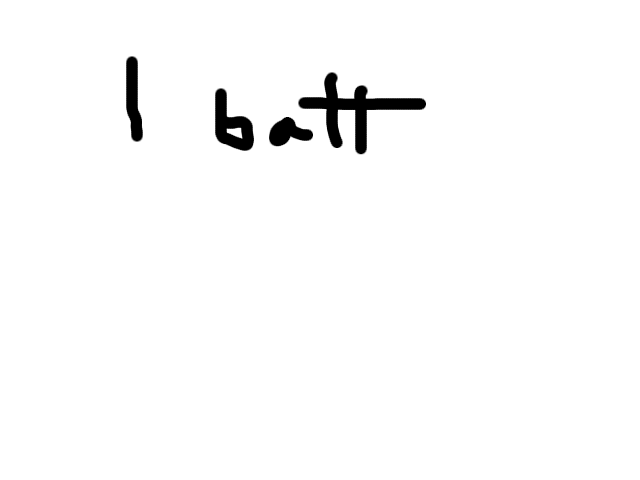
\includegraphics[width=0.4\textwidth]{fig/onebattery}
\caption{Eating \(1\) battery}
\end{figure}

\begin{figure}[h]
\label{fig:fivebatteries}
\centering
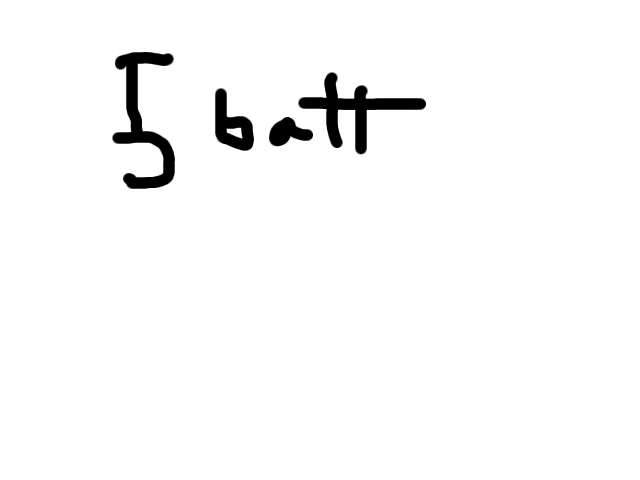
\includegraphics[width=0.4\textwidth]{fig/fivebatteries}
\caption{Eating \(5\) batteries}
\end{figure}

\begin{table}[h]
\label{tab:ssb}
\caption{Captain Falcon}
\centering
\begin{tabular}{r | l}
Falcons & Not Falcons\\
\hline
FALCON & KICK\\
FALCON & KICK\\
FALCON & PUNCH!!
\end{tabular}
\end{table}


\end{document}
\end{verbatim}
\normalsize

This is how appendices are included. In fact, they are written just like
regular chapters, and the \textbackslash appendix flag signals that following
chapters should be given letters (A, B, C...) instead of numbers (1, 2, 3...).

\chapter{Gotchas and Caveats}

\section{Introduction}

\texttt{uafthesis} is not perfect. It still has issues that you need to keep
in mind.

\section{List of Appendices Chicanery}

In an ideal world, \texttt{uafthesis} would write your appendices to the
list of appendices instead of the table of contents. This is currently a bug,
and will be fixed in the future.

The workaround is this:

\begin{enumerate}
\item After generating a pretty-much-done thesis, open up the .toc file. In
this case, the file is called ``example.toc.'' Also open up a corresponding
.loa file (``example.loa'').
\item Cut the lines that refer to appendices out of the .toc file and paste
them into the .loa file. Save both. Make sure the first line in the .loa
that adds "Page" above the pages column stays put.
\item \emph{Make backups of both files.} This is because \LaTeX will overwrite
the .toc file in the next step.
\item Compile (\texttt{pdflatex example}) \emph{exactly once.}
\end{enumerate}

\section{List of Other Materials}

A similar process applies to the List of Other Materials as well:

\begin{quotation}
{ \it ``If you add a pocket or anything else to your thesis (like a CD-ROM)
then you have to have one more List in the Table of Contents.  Follow
the exact same procedure as in step 14, but now you must add the
command:

\textbackslash listofothermaterials

Notice that this goes before the \textbackslash listofappendices.  The file that you
must edit is the thesis12.lom file.  You have to create this by hand.
It is simple.  Here is the example:

\textbackslash renewcommand\textbackslash @pnumwidth\{3.55em\}
\textbackslash contentsline \{section\}{\textbackslash numberline \{A\}CD-ROM of Thesis, Defense and Sandpile Code\}\{Pocket\}
\textbackslash renewcommand\textbackslash @pnumwidth\{1.55em\}

Again, once you save this and run latex once, it will be erased.  A
good habit is to make thesis12.lom.bak and thesis12.loa.bak so they
will always be there.  Then copy them to thesis12.lom and thesis12.loa
and run latex your final time.

I did the \textbackslash @pnumwidth stuff above because the word `Pocket' is wider
than is allowed for a page number.  So I changed it just for this one
line and then changed it back to what it was (as found in the
uafthesis2004.cls file).''\\
\hspace*{1in}---Ryan Woodard
\end{quotation}

I suspect that there's a better way to do this, but I haven't gotten that far
yet.

\section{Bibliography Listings}

If you use \texttt{chapterbib}, also use \texttt{tocbibind} to make sure that
your bibliographies show up in the Table of Contents.

\end{verbatim}
\normalsize

After inputting a few more pages, the chapters (separate documents) are all
included.

\small
\begin{verbatim}
\nocite{wikibook}
\bibliographystyle{agufull08}
\bibliography{thesis}
\end{verbatim}
\normalsize

This generates the bibliography. Note that the bibliography style is set to
\texttt{agufull08}. Generally, the graduate school isn't picky about 
bibliography style, as long as it's consistent. For geophysics papers (very
common at UAF), the AGU style is a great choice. It is included here, but may
also be found at AGU's web site.

\small
\begin{verbatim}
\appendix
\chapter{Extraneous Images and Tables}

\begin{figure}[h]
\label{fig:onebattery}
\centering
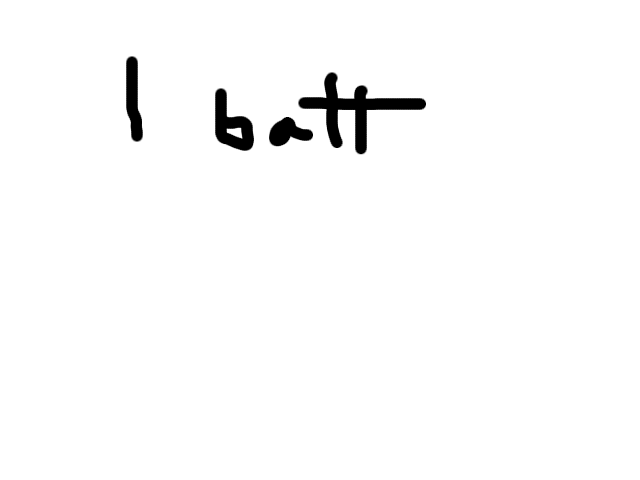
\includegraphics[width=0.4\textwidth]{fig/onebattery}
\caption{Eating \(1\) battery}
\end{figure}

\begin{figure}[h]
\label{fig:fivebatteries}
\centering
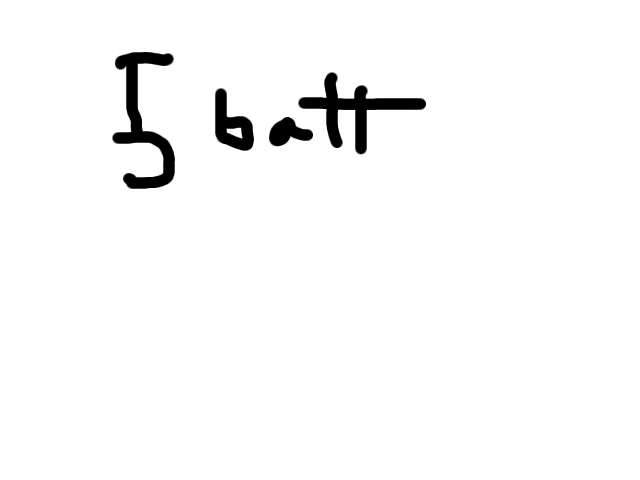
\includegraphics[width=0.4\textwidth]{fig/fivebatteries}
\caption{Eating \(5\) batteries}
\end{figure}

\begin{table}[h]
\label{tab:ssb}
\caption{Captain Falcon}
\centering
\begin{tabular}{r | l}
Falcons & Not Falcons\\
\hline
FALCON & KICK\\
FALCON & KICK\\
FALCON & PUNCH!!
\end{tabular}
\end{table}


\end{document}
\end{verbatim}
\normalsize

This is how appendices are included. In fact, they are written just like
regular chapters, and the \textbackslash appendix flag signals that following
chapters should be given letters (A, B, C...) instead of numbers (1, 2, 3...).

%     \chapter{Gotchas and Caveats}

\section{Introduction}

\texttt{uafthesis} is not perfect. It still has issues that you need to keep
in mind.

\section{List of Appendices Chicanery}

In an ideal world, \texttt{uafthesis} would write your appendices to the
list of appendices instead of the table of contents. This is currently a bug,
and will be fixed in the future.

The workaround is this:

\begin{enumerate}
\item After generating a pretty-much-done thesis, open up the .toc file. In
this case, the file is called ``example.toc.'' Also open up a corresponding
.loa file (``example.loa'').
\item Cut the lines that refer to appendices out of the .toc file and paste
them into the .loa file. Save both. Make sure the first line in the .loa
that adds "Page" above the pages column stays put.
\item \emph{Make backups of both files.} This is because \LaTeX will overwrite
the .toc file in the next step.
\item Compile (\texttt{pdflatex example}) \emph{exactly once.}
\end{enumerate}

\section{List of Other Materials}

A similar process applies to the List of Other Materials as well:

\begin{quotation}
{ \it ``If you add a pocket or anything else to your thesis (like a CD-ROM)
then you have to have one more List in the Table of Contents.  Follow
the exact same procedure as in step 14, but now you must add the
command:

\textbackslash listofothermaterials

Notice that this goes before the \textbackslash listofappendices.  The file that you
must edit is the thesis12.lom file.  You have to create this by hand.
It is simple.  Here is the example:

\textbackslash renewcommand\textbackslash @pnumwidth\{3.55em\}
\textbackslash contentsline \{section\}{\textbackslash numberline \{A\}CD-ROM of Thesis, Defense and Sandpile Code\}\{Pocket\}
\textbackslash renewcommand\textbackslash @pnumwidth\{1.55em\}

Again, once you save this and run latex once, it will be erased.  A
good habit is to make thesis12.lom.bak and thesis12.loa.bak so they
will always be there.  Then copy them to thesis12.lom and thesis12.loa
and run latex your final time.

I did the \textbackslash @pnumwidth stuff above because the word `Pocket' is wider
than is allowed for a page number.  So I changed it just for this one
line and then changed it back to what it was (as found in the
uafthesis2004.cls file).''\\
\hspace*{1in}---Ryan Woodard
\end{quotation}

I suspect that there's a better way to do this, but I haven't gotten that far
yet.

\section{Bibliography Listings}

If you use \texttt{chapterbib}, also use \texttt{tocbibind} to make sure that
your bibliographies show up in the Table of Contents.

%   \end{document}
% \end{verbatim}
% will process only the file \texttt{ch2.tex} as though the files
% \texttt{ch1.tex} and \texttt{ch3.tex} were also present. That is, all
% counters, especially the page and section numbers, as well as
% cross-referencing definitions, will function as if the whole document
% were processed. The trick is that each |\include|d file has it own
% \texttt{.aux} file containing these definitions, and they are all read
% in every time, even if the corresponding \texttt{.tex} file is not. The
% \texttt{.aux} files also contain the citation information for \btx,
% something that the \texttt{chapterbib} package exploits.
%
% If |\usepackage{chapterbib}| has been given, the keys in each |\cite|
% and |\bibitem| command are associated with the current |\include|d file
% and are distinguished from the identical key in a different file. Each of
% these files must contain its own |\bibliography| and |\bibliographystyle|
% commands. One processes \btx\ on each file separately before processing
% it under \LaTeX\ (at least twice).
%
% \subsubsection{Special Considerations for \thestyle\ and
%           \texttt{chapterbib}}

The order in which the \texttt{chapterbib} and \thestyle\ packages are loaded
is unimportant.

The \texttt{chapterbib} package provides an option \texttt{sectionbib}
that puts the bibliography in a |\section*| instead of |\chapter*|,
something that makes sense if there is a bibliography in each chapter.
This option will not work when \thestyle\ is also loaded; instead, add
the option to \thestyle.
% (The \texttt{sectionbib} option can always be
% given, but it only has meaning for the \texttt{book} and \texttt{report}
% classes, or for classes derived from them.)

Every |\include|d file must contain its own
|\bibliography| command where the bibliography is to appear. The database
files listed as arguments to this command can be different in each file,
of course. However, what is not so obvious, is that each file must also
contain a |\bibliographystyle| command, with possibly differing arguments.

As of version~8.0, the citation style, including mode (author--year or
numerical) may also differ between chapters. The |\setcitestyle| command
% as well as |\bibpunct| and |\citestyle|
can be issued at any point in the document, in particular in different
chapters.
%(And this is the only time it would make sense to do so.)
%
% \iffalse
%</notes>
% \fi
%
% \subsection{Sorting and Compressing Numerical Citations}
% \label{sec:sort}
%
% Another package by Donald Arseneau, \texttt{cite.sty}, reimplements the
% entire (numerical) citation system such that one can control the
% punctuation and citation format, all of which is done by \thestyle\ as
% well. However, it also can sort and compress numerical citations,
% something that is required by some journals.
%
% What this means is that when multiple citations are given with a single
% |\cite| command, the normal order of the numbers is in the sequence
% given. This is usually a wild list of numbers, such as [4,2,8,3]. With
% the \texttt{cite} package, this list becomes [2--4,8].
%
% It is impossible to make the \texttt{cite} and \thestyle\ packages
% compatible, since both reimplement |\cite| from scratch. Instead, I have
% taken over some of the coding from \texttt{cite.sty}, modifying it for
% \thestyle{}. This coding is activated by including one of the options
% \texttt{sort} or \texttt{sort\&compress} in the |\usepackage| command.
%
% For author--year citations, the option \texttt{sort} orders the citations in
% a single |\citep| or |\citet| command into the sequence in which they appear
% in the list of references. This is normally alphabetical first, year second.
% This should avoid citations of the type: ``James et~al.\ (1994b,a)''. For
% author--year mode, the \texttt{sort\&compress} option is identical to
% \texttt{sort}.
%
% \iffalse
%<*notes>
\head{Sorting and compressing citations}
Do not use the \texttt{cite} package with \thestyle; rather use one of the
options \texttt{sort}, \texttt{compress}, or \texttt{sort\&compress}.

These also work with author--year citations, making multiple citations appear
in their order in the reference list.

%</notes>
% \fi
%
% \subsection{Merged Numerical References}
% \label{sec:merge}

% \iffalse
%<*notes>
\head{Merged Numerical References}
Do not use the \texttt{mcite} package with \thestyle; rather use the package option \texttt{merge}.

%</notes>
% \fi
% \begin{quote}
% \textbf{Note:} the |merge| coding was contributed by
% Arthur Ogawa for the American Physical Society.
% \end{quote}
%
% Thorsten Ohl's \texttt{mcite} package cannot be used together with
% \thestyle. Instead, one must invoke the package option
% \texttt{merge} with the |\usepackage| statement.
%
% \iffalse
%<*notes>
% \fi

With this option in effect, citation keys within a multiple |\citep| command
may contain a leading * that causes them to be merged in the bibliography
together with the previous citation as a single entry with a single reference
number. For example, |\citep{feynmann,*salam,*epr}| produces a single number,
and all three references are listed in the bibliography under one entry with
that number.
%
% Certain restrictions of Thorsten Ohl's \texttt{mcite} package are lifted: a *
% prefix can be used with any citation key, and Ohl's restrictions on syntax do
% not apply.
%
% An additional feature allows text to be inserted inside the bibliography entry:
% within the argument of \verb+\citep+, a cite key may be preceded by two optional arguements, e.g.,
% \verb+\citep{[+\emph{pre}\verb+][+\emph{post}\verb+]+\emph{key}\verb+}+,
% where \emph{pre} represents text to be prepended to the reference (\verb+\bibitem+ content),
% with \emph{post} appended thereto.
%
% Thus it is possible for the user to mark up the document:
% \begin{verbatim}
% text \citep{*[{See, e.g., }][ for a simpler explanation]ablebaker}
% \end{verbatim}
% The above example illustrates the use of the star-form and both optional arguments.
%
% \medskip\noindent
% \textbf{Caution:} Because the comma (,) character is part of the syntax of \verb+\citep+,
% and because the bracket delimiters ([]) are mere text characters and not true delimiters (like the braces),
% you must enclose the optional argument in braces (\verb+{}+) if a comma is present in the
% argument (that goes for brackets, too, of course).

The \texttt{elide} option also activates the merging features, but also sees
to it that common parts of the merged references (e.g., authors) are not
repeated but are written only once in the single bibliography entry.

The \texttt{mcite} option turns off the merging and eliding features, but
allows the special syntax (the * and optional inserted texts) to be ignored.

These functions are available only to numerical-mode citations, and only when
used parenthetically, similar to the restrictions on \texttt{sort} and
\texttt{compress}.

They also require special \texttt{.bst} files, as provided for example by the
American Physical Society for their REV\TeX\ class.
% \iffalse
%</notes>
% \fi
%
% \subsection{Long Author List on First Citation}\label{sec:long}
%
% A feature that has often been requested by otherwise happy users of
% \thestyle\ is one that is found in the \texttt{harvard} package as
% standard: with the first citation of any reference, the full author list is
% printed, and afterwards only the abbreviated list. One can control this
% with |\citet*| for the first citation, and |\citet| or |\citep| thereafter.
% However, the automatic feature is very desired.
%
% This can be activated with the option
% \texttt{longnamesfirst}.
%
% \iffalse
%<*notes>
\head{Long author list on first citation}
Use option \texttt{longnamesfirst} to have first citation automatically give
the full list of authors.

Suppress this for certain citations with |\shortcites{|\emph{key-list}|}|,
given before the first citation.

%</notes>
% \fi
%
% \DescribeMacro{\shortcites}
% Some references have so many authors that you want to suppress the
% automatic long list only for them. In this case, issue
% \begin{quote}
%   |\shortcites|\marg{key-list}
% \end{quote}
% before the first citations, and those included in \emph{key-list} will have
% a short list on their first citation.
%
% Full author lists can still be forced at any time with the starred
% variants.
%
% \section{Numerical Citations with Author--Year Styles}\label{sec:6.0}
%
% It is possible to produce numerical citations with any author-year
% \texttt{.bst} file, with minimal change to the text. The commands |\citet|
% and |\citep| will produce sensible results in both modes, without any special
% editing. Obviously, the opposite is not possible; a \texttt{.bst} file
% intended for numerical citation can never produce author--year citations,
% simply because the information is not transferred to the auxiliary file.
%
% \subsection{Selecting Numerical Mode}
% By default, \thestyle{} is in author--year mode. This can be changed by
% \begin{enumerate}
%   \item selecting a numerical bibliography style with predefined
%         citation style, defined either in the package or in the local
%         configuration file;
%
%   \item giving options \texttt{numbers} or \texttt{super} to the
%         |\usepackage| command;
%
%   \item issuing |\setcitestyle{numbers}|;
%
%   \item issuing |\citestyle| with the name of a predefined numerical
%         bibliography style (like \texttt{plain} and use it with \texttt{plainnat}).
% \end{enumerate}
%
% The \thestyle{} package will automatically switch to numerical mode if
% any one of the |\bibitem| entries fails to conform to the possible
% author--year formats. There is no way to override this, since such an
% entry would cause trouble in the author--year mode.
%
% There are certain special `numerical' styles, like that of the standard
% \texttt{alpha.bst}, which include a non-numerical label in place of the
% number, in the form
% \begin{quote} |\bibitem[ABC95]{able95}| \end{quote}
% As far as \thestyle\ is concerned, this label does not conform to the
% author--year possibilities and is therefore considered to be numerical.
% The citation mode switches to numerical, and |\cite{able95}| prints
% [ABC95].
%
% See however, the end of Section~\ref{sec:yearless} for another possibility.
% The above result can be achieved with
% \begin{quote} |\bibitem[ABC95()]{able95}| \end{quote}
%
% \section{Local Configuration}
% It is possible to add a local configuration file
% \thestyle\texttt{.cfg}, which is read in, if it exists, at
% the end of the package. It may thus contain coding to supecede that in
% the package, although its main purpose is to allow the user to add his or her
% own |\bibstyle@|\textit{bst} definitions to couple citation punctuation
% with local bibliography styles or for use with |\citestyle|.
%
% \iffalse
%<*notes>
\head{Local configuration}
Any local recoding or definitions can be put in \thestyle\texttt{.cfg} which
is read in after the main package file.

%</notes>
% \fi
%
% \section{Package Options}\label{sec:opts}
% When a package is loaded with |\usepackage|, one can add options to select
% different features, as
% \begin{quote}
% |\usepackage[|\emph{options}|]{|\thestyle|}|
% \end{quote}
% \iffalse
%<*notes>
\head{Options that can be added to \texttt{\char`\\ usepackage}}
% \fi
% The options available provide another means of specifying the
% punctuation for citations:
\begin{description}
\item[\ttfamily round] (default) for round parentheses;
\item[\ttfamily square] for square brackets;
\item[\ttfamily curly] for curly braces;
\item[\ttfamily angle] for angle brackets;
\item[\ttfamily semicolon] (default) to separate multiple citations with
     semi-colons;
\item[\ttfamily colon] the same as \texttt{semicolon}, an earlier mistake in
     terminology;
\item[\ttfamily comma] to use commas as separators;
\item[\ttfamily authoryear] (default) for author--year citations;
\item[\ttfamily numbers] for numerical citations;
\item[\ttfamily super] for superscripted numerical citations, as in
     \textsl{Nature};
\item[\ttfamily sort] orders multiple citations into the sequence in
     which they appear in the list of references;
\item[\ttfamily sort\&compress] as \texttt{sort} but in addition multiple
     numerical citations are compressed if possible (as 3--6, 15);
\item[\ttfamily compress] to compress without sorting, so compression only
     occurs when the given citations would produce an ascending sequence of
     numbers;
\item[\ttfamily longnamesfirst] makes the first citation of any reference
     the equivalent of the starred variant (full author list) and subsequent
     citations normal (abbreviated list);
\item[\ttfamily sectionbib] redefines |\thebibliography| to issue
     |\section*| instead of |\chapter*|; valid only for classes with a
     |\chapter| command; to be used with the \texttt{chapterbib} package;
\item[\ttfamily nonamebreak] keeps all the authors' names in a citation on
     one line; causes overfull hboxes but helps with some \texttt{hyperref}
     problems;
\item[\ttfamily merge] to allow the * prefix to the citation key,
     and to merge such a citation's reference with that of the previous
     citation;
\item[\ttfamily elide] to elide common elements of merged references, like
     the authors or year;
\item[\ttfamily mcite] to recognize (and ignore) the merging syntax.
\end{description}
% The options \texttt{curly} and \texttt{angle} are not really serious; I only
% added them because that completes the normal list of bracket types. The only
% other citation possibilities I know have really encountered are solidus, e.g. /21/,
% or something like (Ref. 21). These must be set with |\setcitestyle{open={/},close={/}}|.
% \iffalse
%</notes>
% \fi
%
% The package options are overwritten by any explicit |\setcitestyle|, |\bibpunct|,
% or |\citestyle| commands. And both these commands and the package options
% turn off the automatic setting with |\bibliographystyle|, if effective.
%
% \section{Reference Sheet}
%
% A summary of the main points on using \thestyle\ can be obtained by
% \LaTeX{}ing the file \texttt{natnotes.tex}, which is extracted from the main
% source file \thestyle\texttt{.dtx} with the \texttt{docstrip} option
% \texttt{notes}. This is intended to act as a handy reference sheet.
%
% This file should be extracted automatically by the supplied installation file,
% \thestyle\texttt{.ins}.
%
%^^A The following is a summary that goes into the .sty file
%^^A It is not printed in the documentation, since the Reference Sheet exists
% \iffalse
%<*package>
 % This package reimplements the LaTeX \cite command to be used for various
 % citation styles, both author-year and numerical. It accepts BibTeX
 % output intended for many other packages, and therefore acts as a
 % general, all-purpose citation-style interface.
 %
 % With standard numerical .bst files, only numerical citations are
 % possible. With an author-year .bst file, both numerical and
 % author-year citations are possible.
 %
 % If author-year citations are selected, \bibitem must have one of the
 %   following forms:
 %   \bibitem[Jones et al.(1990)]{key}...
 %   \bibitem[Jones et al.(1990)Jones, Baker, and Williams]{key}...
%<*apalike|all>
 %   \bibitem[Jones et al., 1990]{key}...
%</apalike|all>
%<*newapa|chicago|all>
 %   \bibitem[\protect\citeauthoryear{Jones, Baker, and Williams}{Jones
 %       et al.}{1990}]{key}...
 %   \bibitem[\protect\citeauthoryear{Jones et al.}{1990}]{key}...
%</newapa|chicago|all>
%<*astron|all>
 %   \bibitem[\protect\astroncite{Jones et al.}{1990}]{key}...
%</astron|all>
%<*authordate|all>
 %   \bibitem[\protect\citename{Jones et al., }1990]{key}...
%</authordate|all>
%<*harvard|all>
 %   \harvarditem[Jones et al.]{Jones, Baker, and Williams}{1990}{key}...
%</harvard|all>
 %
 % This is either to be made up manually, or to be generated by an
 % appropriate .bst file with BibTeX.
 %                            Author-year mode     ||   Numerical mode
 % Then, \citet{key}  ==>>  Jones et al. (1990)    ||   Jones et al. [21]
 %       \citep{key}  ==>> (Jones et al., 1990)    ||   [21]
 % Multiple citations as normal:
 % \citep{key1,key2}  ==>> (Jones et al., 1990; Smith, 1989) || [21,24]
 %                           or  (Jones et al., 1990, 1991)  || [21,24]
 %                           or  (Jones et al., 1990a,b)     || [21,24]
 % \cite{key} is the equivalent of \citet{key} in author-year mode
 %                         and  of \citep{key} in numerical mode
 % Full author lists may be forced with \citet* or \citep*, e.g.
 %       \citep*{key}      ==>> (Jones, Baker, and Williams, 1990)
 % Optional notes as:
 %   \citep[chap. 2]{key}    ==>> (Jones et al., 1990, chap. 2)
 %   \citep[e.g.,][]{key}    ==>> (e.g., Jones et al., 1990)
 %   \citep[see][pg. 34]{key}==>> (see Jones et al., 1990, pg. 34)
 %  (Note: in standard LaTeX, only one note is allowed, after the ref.
 %   Here, one note is like the standard, two make pre- and post-notes.)
 %   \citealt{key}          ==>> Jones et al. 1990
 %   \citealt*{key}         ==>> Jones, Baker, and Williams 1990
 %   \citealp{key}          ==>> Jones et al., 1990
 %   \citealp*{key}         ==>> Jones, Baker, and Williams, 1990
 % Additional citation possibilities (both author-year and numerical modes)
 %   \citeauthor{key}       ==>> Jones et al.
 %   \citeauthor*{key}      ==>> Jones, Baker, and Williams
 %   \citeyear{key}         ==>> 1990
 %   \citeyearpar{key}      ==>> (1990)
 %   \citetext{priv. comm.} ==>> (priv. comm.)
 %   \citenum{key}          ==>> 11 [non-superscripted]
 % Note: full author lists depends on whether the bib style supports them;
 %       if not, the abbreviated list is printed even when full requested.
 %
 % For names like della Robbia at the start of a sentence, use
 %   \Citet{dRob98}         ==>> Della Robbia (1998)
 %   \Citep{dRob98}         ==>> (Della Robbia, 1998)
 %   \Citeauthor{dRob98}    ==>> Della Robbia
 %
 %
 % Citation aliasing is achieved with
 %   \defcitealias{key}{text}
 %   \citetalias{key}  ==>> text
 %   \citepalias{key}  ==>> (text)
 %
 % Defining the citation mode and punctual (citation style)
 %   \setcitestyle{<comma-separated list of keywords, same
 %     as the package options>}
 % Example: \setcitestyle{square,semicolon}
 % Alternatively:
 % Use \bibpunct with 6 mandatory arguments:
 %    1. opening bracket for citation
 %    2. closing bracket
 %    3. citation separator (for multiple citations in one \cite)
 %    4. the letter n for numerical styles, s for superscripts
 %        else anything for author-year
 %    5. punctuation between authors and date
 %    6. punctuation between years (or numbers) when common authors missing
 % One optional argument is the character coming before post-notes. It
 %   appears in square braces before all other arguments. May be left off.
 % Example (and default) \bibpunct[, ]{(}{)}{;}{a}{,}{,}
 %
 % To make this automatic for a given bib style, named newbib, say, make
 % a local configuration file, natbib.cfg, with the definition
 %   \newcommand{\bibstyle@newbib}{\bibpunct...}
 % Then the \bibliographystyle{newbib} will cause \bibstyle@newbib to
 % be called on THE NEXT LATEX RUN (via the aux file).
 %
 % Such preprogrammed definitions may be invoked anywhere in the text
 %  by calling \citestyle{newbib}. This is only useful if the style specified
 %  differs from that in \bibliographystyle.
 %
 % With \citeindextrue and \citeindexfalse, one can control whether the
 % \cite commands make an automatic entry of the citation in the .idx
 % indexing file. For this, \makeindex must also be given in the preamble.
 %
 % Package Options: (for selecting punctuation)
 %   round  -  round parentheses are used (default)
 %   square -  square brackets are used   [option]
 %   curly  -  curly braces are used      {option}
 %   angle  -  angle brackets are used    <option>
 %   semicolon  -  multiple citations separated by semi-colon (default)
 %   colon  - same as semicolon, an earlier confusion
 %   comma  -  separated by comma
 %   authoryear - selects author-year citations (default)
 %   numbers-  selects numerical citations
 %   super  -  numerical citations as superscripts
 %   sort   -  sorts multiple citations according to order in ref. list
 %   sort&compress   -  like sort, but also compresses numerical citations
 %   compress - compresses without sorting
 %   longnamesfirst  -  makes first citation full author list
 %   sectionbib - puts bibliography in a \section* instead of \chapter*
 %   merge - allows the citation key to have a * prefix,
 %           signifying to merge its reference with that of the previous citation.
 %   elide - if references are merged, repeated portions of later ones may be removed.
 %   mcite - recognizes and ignores the * prefix for merging.
 % Punctuation so selected dominates over any predefined ones.
 % Package options are called as, e.g.
 %        \usepackage[square,comma]{natbib}
 % LaTeX the source file natbib.dtx to obtain more details
 % or the file natnotes.tex for a brief reference sheet.
 %-----------------------------------------------------------
%</package>
% \fi
%
% \section{Options with \texttt{docstrip}}
% The source \texttt{.dtx} file is meant to be processed with
% \texttt{docstrip}, for which a number of options are available:
% \begin{description}
% \item[\ttfamily all] includes all of the other interfaces;
%
% \item[\ttfamily apalike] allows interpretation of minimal \texttt{apalike}
%    form of |\bibitem|;
%
% \item[\ttfamily newapa] allows |\citeauthoryear| to be in the optional
%    argument of |\bibitem| along with the punctuation commands of
%    \texttt{newapa.sty};
%
% \item[\ttfamily chicago] is the same as \texttt{newapa};
%
% \item[\ttfamily harvard] includes interpretation of |\harvarditem|;
%
% \item[\ttfamily astron] allows |\astroncite| to appear in the optional
%    argument of |\bibitem|;
%
% \item[\ttfamily authordate] adds the syntax of the |\citename| command.
%
% \end{description}
%
% The remaining options are:
% \begin{description}
% \item[\ttfamily package] to produce a \texttt{.sty} package file with most
%     comments removed;
%
% \item[\ttfamily notes] extracts a summary of usage to be used as a
%     reference sheet; the resulting file is to be \LaTeX{}ed;
%
% \item[\ttfamily driver] to produce a driver \texttt{.ltx} file that will
%     print out the documentation when \LaTeX'd. This file can be modified
%     to produce various alternatives (page size, fonts, manual only, or with
%     annotated code). The \thestyle\texttt{.dtx} file is itself such a driver
%     but it should never, ever be edited by a user.
%
% \end{description}
% The source file \texttt{\filename.dtx} is itself a driver file and can
% be processed directly by \LaTeX.
%
%
% \section{Other Author--Year Solutions}
% \begin{quote}\slshape
% This section is of historical interest only.
% \end{quote}
%
% Before \thestyle{} was published in 1993, there were several other attempts
% to provide author--year citations, some of which inspired \thestyle. A few of
% these are still maintained and used, and for that reason, \thestyle{} has
% attempted to include their |\bibitem| syntaxes, to be compatible with those
% \texttt{.bst} files.
%
% Most of these `packages' are really \LaTeX~2.09 style files, so do not have
% features available with the modern \LaTeXe.
%
% \subsection{The \texttt{natsci.bst} Style}
% What gave me my first inspiration was Stephen Gildea's \texttt{natsci.bst}
% for use with his \texttt{agujgr.sty} file. This showed me that the problem
% was solvable. However, Gildea's formats |\bibitem| with just
% the abbreviated
% authors and year. Thus only parenthetical citations can be accommodated.
%
% The name \texttt{natsci} stands for \emph{natural sciences}, and it was this
% that led to the name \thestyle. (This is admittedly an ugly name, but it is
% now established and cannot be changed so easily.)
%
% \subsection{The \texttt{apalike.bst} Style}
% Oren Patashnik, the originator of \btx{} and the standard \texttt{.bst}
% files, has also worked on an author--year style, called \texttt{apalike.bst}
% with a corresponding \texttt{apalike.sty} to support it. Again, only the
% parenthetical citation is provided. Its functionality is identical to that
% of the \texttt{natsci} files.
%
% The form of the \texttt{thebibliography} entries in this system is
% \begin{quote}
% |\bibitem[Jones et al., 1990]{jon90}...|
% \end{quote}
% This is the most minimal form that can
% be given. I name it the \texttt{apalike} variant, after Patashnik's
% \texttt{apalike.bst} and \texttt{apalike.sty}. However, there could be many
% independent \texttt{.bst} files that follow this line, such as the
% \texttt{natsci} styles.
%
% The bibliography style files belonging to this group include:
% \begin{quote}
% \texttt{apalike}, \texttt{apalike2}, \texttt{cea}, \texttt{cell},
% \texttt{jmb}, \texttt{phapalik}, \texttt{phppcf}, \texttt{phrmp}
% \end{quote}
%
% \subsection{The \texttt{newapa} Style}
% A major improvement was achieved with \texttt{newapa.bst} and the
% accompanying \texttt{newapa.sty} files by Stephen N. Spencer and Young U.
% Ryu. Under their system, three separate items of information are included
% in the |\bibitem| label, to be used as required. These are: the full
% author list, the abbreviated list, and the year. This is accomplished by
% means of a |\citeauthoryear| command included in the label, as
% \begin{quote}
% |\bibitem[\protect\citeauthoryear{Jones, Barker,|\\
% |  and Williams}{Jones et al.}{1990}]{jon90}...|
% \end{quote}
% Actually, this only illustrates the basic structure of |\citeauthoryear|;
% the \texttt{newapa} files go even further to replace some words and
% punctuation
% with commands. For example, the word `and' above is really
% |\betweenauthors|, something that must be defined in the \texttt{.sty} file.
% Of course, |\citeauthoryear| is also defined in that file. A
% number of different |\cite| commands are available to print out the
% citation with complete author list, with the short list, with or without
% the date, the textual or parenthetical form.
%
% Thus the |\citeauthoryear| entry in |\bibitem| is very flexible,
% permitting the style file to generate every citation form that one might
% want. It is used by a number of other styles, with corresponding
% \texttt{.sty} files. They all appear to have been inspired by
% \texttt{newapa.bst}, although they lack the extra punctuation commands.
%
% Bibliographic style files belonging to the \texttt{newapa} group include
% \begin{quote}
% \texttt{newapa}, \texttt{chicago}, \texttt{chicagoa}, \texttt{jas99},
% \texttt{named}
% \end{quote}
%
% \noindent
% \textbf{Note:} the last of these, \texttt{named.bst}, uses |\citeauthoryear| in a
% slightly different manner, with only two arguments: the short list and
% year.
%
% \subsection{The Harvard Family}
% The same effect is achieved by a different approach in the Harvard family
% of bibliographic styles. Here a substitute for |\bibitem| is used, as
% \begin{quote}
% |\harvarditem[Jones et al.]{Jones, Baker, and|\\
% |   Williams}{1990}{jon90}...|
% \end{quote}
% The accompanying interface package file is called \texttt{harvard.sty}
% and is written by Peter Williams and Thorsten Schnier. It
% defines |\harvarditem| as well as the citation commands |\cite|, for
% parenthentical, and |\citeasnoun|, for textual citations. The first
% citation uses the long author list, following ones the shorter list, if
% it has been given in the optional argument to |\harvarditem|.
%
% Bibliography styles belonging to the Harvard family are
% \begin{quote}
% \texttt{agsm}, \texttt{dcu}, \texttt{kluwer}
% \end{quote}
%
% This package has been updated for \LaTeXe, with many additions to
% add flexibility. The result is a powerful interface that should meet most
% citation needs. (It does not suppress repeated authors, though,
% as \thestyle{} does.)
%
% \subsection{The Astronomy Style}
% Apparently realizing the limitations of his \texttt{apalike} system, Oren
% Patashnik went on to develop a `true' \texttt{apa} bibliographic style,
% making use of the method already employed by an astronomy journal. This
% is actually very similar to the \texttt{newapa} label but with only the
% short list of authors:
% \begin{quote}
% |\bibitem[\protect\astroncite{Jones et al.}{1990}]{jon90}|\\
% |   ...|
% \end{quote}
% It requires the package file \texttt{astron.sty}
% or any other style that defines |\astroncite| appropriately.
%
% Bibliographic styles belonging to the astronomy group are
% \begin{quote}
% \texttt{apa}, \texttt{astron}, \texttt{bbs}, \texttt{cbe},
% \texttt{humanbio}, \texttt{humannat}, \texttt{jtb}
% \end{quote}
%
% This is as good as the |\citeauthoryear| command, although not as
% flexible since the full list of authors is missing.
%
% \subsection{The \texttt{authordate} Style}
% Finally, I also found some packages making use of a label command
% called |\citename| in the form
% \begin{quote}
% |\bibitem[\protect\citename{Jones et al., }1990]{jon90}|\\
% |    ...|
% \end{quote}
%
% This is not a good system since the author list and date are not cleanly
% separated as individual arguments, and since the punctuation is included
% in the label text. It is better to keep the punctuation fully removed, as
% part of the definitions in the \texttt{.sty} file, for complete flexibility.
%
% Bibliographic styles belonging to this group are
% \begin{quote}
% \texttt{authordate1}, \texttt{authordate2}, \texttt{authordate3},
% \texttt{authordate4}, \texttt{aaai-named}
% \end{quote}
% with accompanying style file \texttt{authordate1-4.sty}.
%
% \iffalse
%<notes>\end{document}
% \fi
%
% \StopEventually{\PrintIndex\PrintChanges}
%
% \section{The Coding}
% This section presents and explains the actual coding of the macros.
% It is nested between |%<*package>| and |%</package>|, which
% are indicators to \texttt{docstrip} that this coding belongs to the package
% file.
%    \begin{macrocode}
%<*package>
%    \end{macrocode}
%
% With \LaTeX\ release from \texttt{1995/12/01}, |\cite| is made robust,
% something that I have adopted as well.
%
% Another change in the above release is that
% |\G@refundefinedtrue|\footnote{In fact, it was only proposed to be
%    removed, but because several packages, including this one, were
%    adversely affected, the name was retained for the new coding.}
% and the |\if@openbib| flag have been removed.
% New, more effective, and compact, coding has replaced them. Rather than
% relying on the kernel coding, I make \thestyle\ more
% self-reliant.
%
% \subsection{Prerequisites}
%
% \begin{macro}{\@ifxundefined}
% \begin{macro}{\@ifnum}
% \begin{macro}{\@ifx}
% \begin{macro}{\appdef}
% \changes{8.2}{2008 Jul 02}{(AO) Add \cs{@ifxundefined}, a tool for testing a
%      \cs{TeX} macro, and \cs{@ifnum}, a tool for testing numbers, like \cs{ifnum}.}
% The test |\@ifxundefined| is similar syntactically to |\@ifundefined|, but
% its first argument is a control sequence name.
%
% A singular disadvantage of |\@ifundefined| is its side effect of
% changing the state of the effective control sequence name, if undefined, to |\relax|.
% In the usual usage of |\@ifundefined|, this does not have serious consequences,
% but it can, and |\@ifxundefined| avoids these.
%
% We also provide |\@ifnum|, a vehicle for |\ifnum| tests, but using the same
% Boolean algebra as, e.g., |\@ifundefined|, with its attendant advantages.
% Likewise, |\@ifx| is the analog to |\ifx|.
%
%    \begin{macrocode}
\providecommand\@ifxundefined[1]{%
 \ifx#1\@undefined\expandafter\@firstoftwo\else\expandafter\@secondoftwo\fi
}%
\providecommand\@ifnum[1]{%
 \ifnum#1\expandafter\@firstoftwo\else\expandafter\@secondoftwo\fi
}%
\providecommand\@ifx[1]{%
 \ifx#1\expandafter\@firstoftwo\else\expandafter\@secondoftwo\fi
}%
\providecommand\appdef[2]{%
 \toks@\expandafter{#1}\@temptokena{#2}%
 \edef#1{\the\toks@\the\@temptokena}%
}%
%    \end{macrocode}
%\end{macro}
%\end{macro}
%\end{macro}
%\end{macro}
%
% \subsection{Test for Specific Journals}
% This package should not be loaded with the specific journal packages that
% already include it; it is superfluous and can lead to contradictions.
%    \begin{macrocode}
\@ifclassloaded{agu2001}{\PackageError{natbib}
  {The agu2001 class already includes natbib coding,\MessageBreak
   so you should not add it explicitly}
  {Type <Return> for now, but then later remove\MessageBreak
   the command \protect\usepackage{natbib} from the document}
  \endinput}{}
\@ifclassloaded{agutex}{\PackageError{natbib}
  {The AGUTeX class already includes natbib coding,\MessageBreak
   so you should not add it explicitly}
  {Type <Return> for now, but then later remove\MessageBreak
   the command \protect\usepackage{natbib} from the document}
  \endinput}{}
\@ifclassloaded{aguplus}{\PackageError{natbib}
  {The aguplus class already includes natbib coding,\MessageBreak
   so you should not add it explicitly}
  {Type <Return> for now, but then later remove\MessageBreak
   the command \protect\usepackage{natbib} from the document}
  \endinput}{}
\@ifclassloaded{nlinproc}{\PackageError{natbib}
  {The nlinproc class already includes natbib coding,\MessageBreak
   so you should not add it explicitly}
  {Type <Return> for now, but then later remove\MessageBreak
   the command \protect\usepackage{natbib} from the document}
  \endinput}{}
\@ifclassloaded{egs}{\PackageError{natbib}
  {The egs class already includes natbib coding,\MessageBreak
   so you should not add it explicitly}
  {Type <Return> for now, but then later remove\MessageBreak
   the command \protect\usepackage{natbib} from the document}
  \endinput}{}
\@ifclassloaded{egu}{\PackageError{natbib}
  {The egu class already includes natbib coding,\MessageBreak
   so you should not add it explicitly}
  {Type <Return> for now, but then later remove\MessageBreak
   the command \protect\usepackage{natbib} from the document}
  \endinput}{}
%    \end{macrocode}
%
% \subsection{Selecting Citation Punctuation and Other Modifications}
% \begin{macro}{\bibstyle@xxx}
% \changes{5.3}{1994 Sep 13}{Add \texttt{agsm} and \texttt{dcu} punctuation
%    styles from \texttt{harvard} series}
% We begin by defining a number of punctuation styles for specific
% author--year \texttt{.bst} files that I use.
% They are placed here, near the beginning, so that another
% user can easily find them to add his own. Some comments remain in the
% stripped version too.
%    \begin{macrocode}
 % Define citation punctuation for some author-year styles
 % One may add and delete at this point
 % Or put additions into local configuration file natbib.cfg
\newcommand\bibstyle@chicago{\bibpunct{(}{)}{;}{a}{,}{,}}
\newcommand\bibstyle@named{\bibpunct{[}{]}{;}{a}{,}{,}}
\newcommand\bibstyle@agu{\bibpunct{[}{]}{;}{a}{,}{,~}}%Amer. Geophys. Union
\newcommand\bibstyle@copernicus{\bibpunct{(}{)}{;}{a}{,}{,}}%Copernicus Publications
\let\bibstyle@egu=\bibstyle@copernicus
\let\bibstyle@egs=\bibstyle@copernicus
%<*all|harvard>
\newcommand\bibstyle@agsm{\bibpunct{(}{)}{,}{a}{}{,}\gdef\harvardand{\&}}
\newcommand\bibstyle@kluwer{\bibpunct{(}{)}{,}{a}{}{,}\gdef\harvardand{\&}}
\newcommand\bibstyle@dcu{\bibpunct{(}{)}{;}{a}{;}{,}\gdef\harvardand{and}}
%</all|harvard>
%    \end{macrocode}
%
% Here give the explicit punctuation for the specific journals; their
% coding need not contain the punctuation macros |\bibpunct| and
% |\bibstyle@xxx| since the punctuation is fixed for them.
%
% Activate citation sorting for the journals.
% \changes{6.8b}{1998 July 2}{Turn off sorting for AGU and EGS}
%    \begin{macrocode}
\newcommand\bibstyle@aa{\bibpunct{(}{)}{;}{a}{}{,}} %Astronomy & Astrophysics
\newcommand\bibstyle@pass{\bibpunct{(}{)}{;}{a}{,}{,}}%Planet. & Space Sci
\newcommand\bibstyle@anngeo{\bibpunct{(}{)}{;}{a}{,}{,}}%Annales Geophysicae
\newcommand\bibstyle@nlinproc{\bibpunct{(}{)}{;}{a}{,}{,}}%Nonlin.Proc.Geophys.
%    \end{macrocode}
%
% \changes{6.5}{1997 Jan 30}{Fix \texttt{esa} style for new note system}
% \changes{7.0}{1999 May 7}{Fix \texttt{esa} style again}
% Next, the same thing is done for some numerical styles. A major
% difference here is that the |\@biblabel| and |\@cite| commands must also
% be redefined in many cases. These redefinitions must be made with the
% |\gdef| (global definition) command.
%    \begin{macrocode}
 % Define citation punctuation for some numerical styles
\newcommand\bibstyle@cospar{\bibpunct{/}{/}{,}{n}{}{}%
     \gdef\bibnumfmt##1{##1.}}
\newcommand\bibstyle@esa{\bibpunct{(Ref.~}{)}{,}{n}{}{}%
     \gdef\bibnumfmt##1{##1.\hspace{1em}}}
\newcommand\bibstyle@nature{\bibpunct{}{}{,}{s}{}{\textsuperscript{,}}%
     \gdef\bibnumfmt##1{##1.}}
%    \end{macrocode}
%
% Finally, the standard \LaTeX{} (numerical) citation styles are included
%  along with their \thestyle\ modifications (author--year).
%    \begin{macrocode}
 % The standard LaTeX styles
\newcommand\bibstyle@plain{\bibpunct{[}{]}{,}{n}{}{,}}
\let\bibstyle@alpha=\bibstyle@plain
\let\bibstyle@abbrv=\bibstyle@plain
\let\bibstyle@unsrt=\bibstyle@plain
 % The author-year modifications of the standard styles
\newcommand\bibstyle@plainnat{\bibpunct{[}{]}{,}{a}{,}{,}}
\let\bibstyle@abbrvnat=\bibstyle@plainnat
\let\bibstyle@unsrtnat=\bibstyle@plainnat
%    \end{macrocode}
% \end{macro}
%
% \subsection{Package Options}
% \begin{macro}{\ifNAT@numbers}
% \changes{5.5}{1995 Mar 21}{Add flag for switching between cite styles}
% \begin{macro}{\ifNAT@super}
% \changes{5.5}{1995 Mar 21}{Add flag for switching between cite styles}
% Two flags are used to keep track of the citation style. The flag
% |\ifNAT@numbers| is \meta{false} by default (author--year) and switches
% to \meta{true} for numerical citations. The flag |\ifNAT@super| indicates
% if the numerical citation is to be done with superscripts.
%
% Note that changing |\ifNAT@numbers| or |\ifNAT@super|
% in the body of the text
% will not alter the way the citations are processed;
% their values at the end of the preamble determine the citation style for the
% rest of the document.
%    \begin{macrocode}
\newif\ifNAT@numbers \NAT@numbersfalse
\newif\ifNAT@super \NAT@superfalse
%    \end{macrocode}
% \end{macro}\end{macro}
%
% \begin{macro}{\NAT@merge}
% \changes{8.2}{2008 Jan 10}{(AO)Introduce \texttt{merge} package option}
% The package option |merge| allows multiple references to be merged under a single number
% in the bibliography, inspired by Thorsten Ohl's |mcite| package for \LaTeX.
% New syntax for the |\cite| command: e.g., |\cite{latex,*latex-companion}|,
% where the * signifies that the \LaTeX\ Companion and \LaTeX, a Document Formatting Language
% appear in the bibliography under the same number.
% |merge| applies only to the numerical citation mode; it is inactive in author-year mode.
% It is by default turned off (|\NAT@merge|${}={}$|\z@|).
% If |\NAT@merge|${}>{}$|\@ne|, all features are turned on.
% If |\NAT@merge|${}={}$|\@ne|, then the * syntax is active, but the merging is not done.
%    \begin{macrocode}
\let\NAT@merge\z@
%    \end{macrocode}
% \end{macro}
%
% \begin{macro}{\DeclareOption}
% \changes{5.0}{1994 May 18}{Add \LaTeXe{} options.}
% \changes{5.3}{1994 Sep 13}{Add options \texttt{angle} and \texttt{curly}}
% \changes{6.0}{1995 Sep 6}{Add option \texttt{bibstyle}}
% \changes{6.0}{1995 Sep 6}{Execute \texttt{nobibstyle} with all options}
% \changes{6.1}{1995 Nov 27}{Add option \texttt{openbib}}
% \changes{6.4}{1996 Sep 1}{Add option \texttt{sectionbib}}
% \changes{6.4}{1996 Sep 13}{Add option \texttt{sort}}
% \changes{6.7}{1997 Jul 14}{Add option \texttt{longnamesfirst}}
% \changes{6.8c}{1998 Jul 14}{Add option \texttt{nonamebreak}}
% \changes{8.0}{2007 Feb 6}{Add option \texttt{semicolon}, same as \texttt{colon}}
% We can define some options to be used with the |\usepackage|
% command that loads the \thestyle{} package. These are an additional means
% of specifying the citation punctuation and scheme.
%
% The standard option \texttt{openbib} is also defined here so that its
% behaviour is entirely under my control. Relying on the standard classes
% can lead to trouble.
% \changes{8.2}{2008 Jul 02}{(AO) The value of \cs{NAT@sort} and \cs{NAT@cmprs}
%   will be \cs{z@} or \cs{@ne}: something created by \cs{chardef}.
%   This works better in \cs{ifnum} tests.}
%    \begin{macrocode}
\DeclareOption{numbers}{\NAT@numberstrue
   \ExecuteOptions{square,comma,nobibstyle}}
\DeclareOption{super}{\NAT@supertrue\NAT@numberstrue
   \renewcommand\NAT@open{}\renewcommand\NAT@close{}
   \ExecuteOptions{nobibstyle}}
\DeclareOption{authoryear}{\NAT@numbersfalse
   \ExecuteOptions{round,semicolon,bibstyle}}
\DeclareOption{round}{%
      \renewcommand\NAT@open{(} \renewcommand\NAT@close{)}
   \ExecuteOptions{nobibstyle}}
\DeclareOption{square}{%
      \renewcommand\NAT@open{[} \renewcommand\NAT@close{]}
   \ExecuteOptions{nobibstyle}}
\DeclareOption{angle}{%
      \renewcommand\NAT@open{$<$} \renewcommand\NAT@close{$>$}
   \ExecuteOptions{nobibstyle}}
\DeclareOption{curly}{%
      \renewcommand\NAT@open{\{} \renewcommand\NAT@close{\}}
   \ExecuteOptions{nobibstyle}}
\DeclareOption{comma}{\renewcommand\NAT@sep{,}
   \ExecuteOptions{nobibstyle}}
\DeclareOption{semicolon}{\renewcommand\NAT@sep{;}
   \ExecuteOptions{nobibstyle}}
\DeclareOption{colon}{\ExecuteOptions{semicolon}}
\DeclareOption{nobibstyle}{\let\bibstyle=\@gobble}
\DeclareOption{bibstyle}{\let\bibstyle=\@citestyle}
\newif\ifNAT@openbib \NAT@openbibfalse
\DeclareOption{openbib}{\NAT@openbibtrue}
\DeclareOption{sectionbib}{\def\NAT@sectionbib{on}}
\def\NAT@sort{\z@}
\def\NAT@cmprs{\z@}
\DeclareOption{sort}{\def\NAT@sort{\@ne}}
\DeclareOption{compress}{\def\NAT@cmprs{\@ne}}
\DeclareOption{sort&compress}{\def\NAT@sort{\@ne}\def\NAT@cmprs{\@ne}}
\DeclareOption{mcite}{\let\NAT@merge\@ne}
\DeclareOption{merge}{\@ifnum{\NAT@merge<\tw@}{\let\NAT@merge\tw@}{}}
\DeclareOption{elide}{\@ifnum{\NAT@merge<\thr@@}{\let\NAT@merge\thr@@}{}}
\@ifpackageloaded{cite}{\PackageWarningNoLine{natbib}
  {The `cite' package should not be used\MessageBreak
   with natbib. Use option `sort' instead}\ExecuteOptions{sort}}{}
\@ifpackageloaded{mcite}{\PackageWarningNoLine{natbib}
  {The `mcite' package should not be used\MessageBreak
   with natbib. Use option `merge' instead}\ExecuteOptions{merge}}{}
\@ifpackageloaded{citeref}{\PackageError{natbib}
  {The `citeref' package must be loaded after natbib}%
  {Move \protect\usepackage{citeref} to after \string\usepackage{natbib}}}{}
\newif\ifNAT@longnames\NAT@longnamesfalse
\DeclareOption{longnamesfirst}{\NAT@longnamestrue}
\DeclareOption{nonamebreak}{\def\NAT@nmfmt#1{\mbox{\NAT@up#1}}}
\def\NAT@nmfmt#1{{\NAT@up#1}}
%    \end{macrocode}
% Before version~6.0, the punctuation options had the lowest priority,
% being overridden by any |\bibstyle@|\textit{bst} command. It was necessary
% to add the option \texttt{nobibstyle} to make them effective. Now this
% option is automatically executed whenever a punctuation option is chosen.
% The reason is that \texttt{nobibstyle} is either superfluous (no
% predefined citation style is present) or always necessary to make the
% other options meaningful.
%
% It seems to be better practice to make any explicit choices to have
% higher priority over implicit ones.
%
% The option \texttt{bibstyle} reactivates the predefined commands, just in
% case this is needed, as it is for the option \texttt{authoryear}. This
% leaves the predefined styles functioning, since it does not really
% determine the citation style, but rather establishes a default which may
% be overwritten by a prestored one.  For this reason, this option must be
% defined very early so that any explicit punctuation options overwrite the
% defaults. (Options are executed in the order defined.)
%
% \end{macro}
%
% \subsection{Selecting Citation Punctuation and Other Modifications}
% \begin{macro}{\bibstyle}
% \changes{5.4}{1994 Nov 24}{Move \cs{ProcessOptions} to after definition
%    of \cs{bibstyle}}
% The pre-defined punctuation styles are associated with particular
% \texttt{.bst} files. This is implemented by means of the standard
% |\bibliographystyle| command that specifies the name of the \texttt{.bst}
% file that is to be used by \btx. Some \LaTeX{} manuals erroneously state
% that this command must be issued prior to any |\cite| commands. If that
% were the case, the task of invoking the style definitions would be much
% easier, for they certainly must be issued before the first |\cite|.
% However, I have always called |\bibliographystyle| together with
% |\bibliography|, well after all |\cite| commands.
%
% In fact, all that |\bibliographystyle|\marg{bst} does is to write
% |\bibstyle|\marg{bst} to the auxiliary file. This file, and all its
% contents, will be read in at the beginning of the next \LaTeX{} run; to
% be precise, it is read in by |\begin{document}|. The command |\bibstyle| is
% then executed at that point on the next run. However, it is
% defined to do nothing more than to swallow up its argument! In other
% words, the combination |\bibliographystyle| and |\bibstyle| do absolutely
% nothing to the \LaTeX{} runs. In fact, |\bibstyle| is a command for
% \btx{} alone.
%
% I have taken advantage of this to redefine |\bibstyle| to execute the
% \texttt{bst}-specific definitions. This definition is made here before
% |\ExecuteOptions| so that options may make use of it; the option
% \texttt{nobibstyle} turns it off, for example.
%
% Coding note (AO): if the csname has not been defined, then executing it simply
% executes |\relax|, so the coding here could be considerably simplified:
% just execute |\csname| |bibstyle@||#1||\endcsname| whether defined or not.
% (Done, PWD)
%    \begin{macrocode}
\renewcommand\bibstyle[1]{\csname bibstyle@#1\endcsname}
%    \end{macrocode}
% This is executed only when the auxiliary file is read in, and that is
% when |\begin{document}| is issued. Thus this is well before any |\cite|
% commands. It is for this reason that any definitions in the
% |\bibstyle@xxx| commands must be global.
%
% A minor problem arises in that the auxiliary file is read in a second
% time, at the end of the run, to check whether any labels have changed.
% Sometimes, re-executing the |\bibstyle@xxx| command at this point
% produces error messages. To avoid this, |\bibstyle| is reset to its
% normal, do-nothing, definition after |\begin{document}|.
%
% (|\NAT@set@cites| must also be executed at the start of the document;
% this is added later when the macro is defined.)
%    \begin{macrocode}
\AtBeginDocument{\global\let\bibstyle=\@gobble}
%    \end{macrocode}
% \end{macro}
%
% \begin{macro}{\citestyle}
% \changes{5.4}{1995 Feb 03}{Add macro}
% \changes{5.5}{1995 Mar 24}{Make preamble only}
% To allow one to invoke preprogrammed punctuation styles that are
% different from the name of the bibliography style specified by
% |\bibliographystyle|, call |\citestyle| in the preamble. This then
% deactivates |\bibstyle| so that any preprogrammed punctuations become
% ineffective.
%
% This, and all other punctuation (citation style) declarations, may only
% be used in the preamble, as of version 5.5. (Previously they could only
% be used after the preamble, but the preamble is more logical.)
%    \begin{macrocode}
\let\@citestyle\bibstyle
\newcommand\citestyle[1]{\@citestyle{#1}\let\bibstyle\@gobble}
%    \end{macrocode}
% \end{macro}
%
% \begin{macro}{\bibpunct}
% \changes{5.4}{1994 Nov 24}{Add superscript style of citations}
% \changes{5.5}{1995 Mar 21}{Use flags to select citation style}
% \changes{5.5}{1995 Mar 24}{Make preamble only}
% \changes{6.0}{1995 Sep 6}{Sets \cs{bibstyle} to \cs{@gobble}}
% \changes{6.0}{1995 Sep 6}{Declare \cs{NAT@numbersfalse} before testing 4th
%      argument}
% \changes{6.0}{1995 Sep 19}{Add optional argument for \cs{NAT@cmt}}
% \changes{7.0}{1999 May 7}{Add blank to default of first argument}
% Now |\bibpunct| is defined. It sets various punctuation commands equal to
% its arguments. It also switches to numerical style if that is specified
% by the fourth argument. This is done by setting the citation style
% flag |NAT@numbers| accordingly. The internal cite macros are later
% set to the style-dependent definitions by calling |\NAT@set@cites|.
%
% The fourth argument can also be \texttt{s} for superscript, which
% sets both the numerical and the |\NAT@super| flags.
%
% An optional argument has been added to determine the punctuation that
% precedes a trailing note. This makes the counting of mandatory arguments
% somewhat confused, since the fourth argument is now |#5|.
%
%    \begin{macrocode}
\newcommand\bibpunct[7][, ]%
  {\gdef\NAT@open{#2}\gdef\NAT@close{#3}\gdef
   \NAT@sep{#4}\global\NAT@numbersfalse
     \ifx #5n\global\NAT@numberstrue\global\NAT@superfalse
   \else
     \ifx #5s\global\NAT@numberstrue\global\NAT@supertrue
   \fi\fi
   \gdef\NAT@aysep{#6}\gdef\NAT@yrsep{#7}%
   \gdef\NAT@cmt{#1}%
   \NAT@@setcites
  }
%    \end{macrocode}
% The command turns off |\bibstyle| so that the predefined
% |\bibstyle@|\textit{bst} commands no longer work. Thus |\bibpunct| has
% priority over the predefined styles.
% \end{macro}
%
% \begin{macro}{\setcitestyle}
% \changes{8.0}{2007 Feb 2}{Add macro}
% A new command for setting the various parameters is added in version~8.0.
% This complements |\bibpunct| but will not replace it since it only sets
% selected parameters, while |\bibpunct| sets all at once, and is thus more
% appropriate for complete setting. This is better for changing just some
% parameters.
%
% The argument is a comma-separated list of keywords, many identical to the
% corresponding package options. However, others take an argument, as
% |yysep={;}| where the curly braces are unnecessary for a single character
% (except for a comma!) but they do not hurt. Spaces must not appear between
% entries, or they will be interpreted as part of the keyword.
%
%    \begin{macrocode}
\newcommand\setcitestyle[1]{
 \@for\@tempa:=#1\do
 {\def\@tempb{round}\ifx\@tempa\@tempb
    \renewcommand\NAT@open{(}\renewcommand\NAT@close{)}\fi
  \def\@tempb{square}\ifx\@tempa\@tempb
    \renewcommand\NAT@open{[}\renewcommand\NAT@close{]}\fi
  \def\@tempb{angle}\ifx\@tempa\@tempb
    \renewcommand\NAT@open{$<$}\renewcommand\NAT@close{$>$}\fi
  \def\@tempb{curly}\ifx\@tempa\@tempb
    \renewcommand\NAT@open{\{}\renewcommand\NAT@close{\}}\fi
  \def\@tempb{semicolon}\ifx\@tempa\@tempb
    \renewcommand\NAT@sep{;}\fi
  \def\@tempb{colon}\ifx\@tempa\@tempb
    \renewcommand\NAT@sep{;}\fi
  \def\@tempb{comma}\ifx\@tempa\@tempb
    \renewcommand\NAT@sep{,}\fi
  \def\@tempb{authoryear}\ifx\@tempa\@tempb
    \NAT@numbersfalse\fi
  \def\@tempb{numbers}\ifx\@tempa\@tempb
    \NAT@numberstrue\NAT@superfalse\fi
  \def\@tempb{super}\ifx\@tempa\@tempb
    \NAT@numberstrue\NAT@supertrue\fi
  \expandafter\NAT@find@eq\@tempa=\relax\@nil
  \if\@tempc\relax\else
    \expandafter\NAT@rem@eq\@tempc
    \def\@tempb{open}\ifx\@tempa\@tempb
     \xdef\NAT@open{\@tempc}\fi
    \def\@tempb{close}\ifx\@tempa\@tempb
     \xdef\NAT@close{\@tempc}\fi
    \def\@tempb{aysep}\ifx\@tempa\@tempb
     \xdef\NAT@aysep{\@tempc}\fi
    \def\@tempb{yysep}\ifx\@tempa\@tempb
     \xdef\NAT@yrsep{\@tempc}\fi
    \def\@tempb{notesep}\ifx\@tempa\@tempb
     \xdef\NAT@cmt{\@tempc}\fi
    \def\@tempb{citesep}\ifx\@tempa\@tempb
     \xdef\NAT@sep{\@tempc}\fi
  \fi
 }%
 \NAT@@setcites
}
 \def\NAT@find@eq#1=#2\@nil{\def\@tempa{#1}\def\@tempc{#2}}
 \def\NAT@rem@eq#1={\def\@tempc{#1}}
%    \end{macrocode}
%
% After the parameters are set, it is still necessary to issue |\NAT@set@cites|
% to get things right for author--year or numerical mode. This is issued
% at the end of the preamble, and not in the preamble. But if |\setcitestyle| is
% given after the preamble, we need it right away. So issue instead |\NAT@@setcites|
% which in the preamble only deactivates |\bibstyle|, but later becomes
% |\NAT@set@cites|.
%
% The idea is that if |\setcitestyle| is used in the preamble, it is global and
% the values should be not changed by the bibliography style definitions. But if
% issued in the text, as part of \texttt{chapterbib} processing, then automatic
% style changes with different |.bst| files per chapter could be useful.
%    \begin{macrocode}
 \def\NAT@@setcites{\global\let\bibstyle\@gobble}
\AtBeginDocument{\let\NAT@@setcites\NAT@set@cites}
%    \end{macrocode}
% \end{macro}
%
% \subsection{Setting the Defaults}
% The defaults (punctuation and scheme type) are set with the
% |\ExecuteOptions| command.
%
% \begin{macro}{\NAT@open}
% \changes{5.5}{1995 May 14}{Renamed from \cs{@citebegin}}
% \begin{macro}{\NAT@close}
% \changes{5.5}{1995 May 14}{Renamed from \cs{@citeend}}
% \begin{macro}{\NAT@sep}
% \changes{5.5}{1995 May 14}{Renamed from \cs{@citesep}}
% \begin{macro}{\NAT@aysep}
% \changes{5.5}{1995 May 14}{Renamed from \cs{@auyrsep}}
% \begin{macro}{\NAT@yrsep}
% \changes{5.5}{1995 May 14}{Renamed from \cs{@yrsep}}
% \begin{macro}{\NAT@cmt}
% \changes{6.0}{1995 Sep 19}{Add macro}
% \changes{6.9}{1999 Feb 25}{Remove hardwired spaces after \cs{NAT@cmt},
%      adding them to default definition instead}
% The five punctuation characters for citations are the start and stop
% brackets, the character between multiple citations, the character between
% the authors and year (parenthetical only), and the character between
% adjacent years when the common author list is omitted.
% A sixth one has been added: the character preceding post-notes,
% including any possible space.
% Define their default values.
%    \begin{macrocode}
\newcommand\NAT@open{(} \newcommand\NAT@close{)}
\newcommand\NAT@sep{;}
%    \end{macrocode}
% \end{macro}\end{macro}\end{macro}\end{macro}\end{macro}\end{macro}
% \changes{6.0}{1995 Sep 19}{Remove \cs{ExecuteOptions} since default
%        style determined by definitions}
% The option \texttt{authoryear} was originally provided to serve as the
% default; hence its definition includes \texttt{bibstyle}. However, this
% is not necessary since all the appropriate parameters are set to these
% values anyway. (One could consider removing \texttt{bibstyle}.)
%    \begin{macrocode}
%\ExecuteOptions{authoryear}
\ProcessOptions
\newcommand\NAT@aysep{,} \newcommand\NAT@yrsep{,}
\newcommand\NAT@cmt{, }
%    \end{macrocode}
%
% \subsection{Internal Citing Macros}
% A number of internal macros (|\@citex|, |\@cite|, |\@biblabel|, and
% |\@bibsetup|) need to have different definitions for author--year and
% numerical schemes. They are defined here for the two different styles,
% with different names, and which ones become active depend on the citation
% style flags |\ifNAT@numbers| and |\ifNAT@super|.
%
% The coding for the journals always defines the internal macros directly
% as the author--year version, since they can never do any switching.
%
% \begin{macro}{\@cite}
% \changes{5.5}{1995 Mar 21}{Is \cs{let} equal to the numerical or
%      author--year definition}
% \begin{macro}{\NAT@cite}
% \changes{4.2}{1993 Dec 2}{Reversed optional text no longer needs to include
%       a trailing blank}
% \changes{5.0}{1994 May 18}{Add optional notes after as well as before
%      citation.}
% \changes{5.5}{1995 Mar 13}{Add command space in place of space}
% \changes{5.5}{1995 Mar 13}{Use \cs{if}\cs{relax}\texttt{\#2}\cs{relax}
%    in place of \cs{if}\texttt{\#2}\cs{@empty}}
% \changes{5.5}{1995 Mar 21}{Renamed from \cs{@cite}}
% \changes{6.6}{1997 May 26}{Use flag \cs{ifNAT@par} to suppress braces
%     optionally}
% \changes{6.8}{1998 Feb 19}{Add \cs{endgroup} to terminate group}
% \changes{6.9a}{1999 Apr 20}{Change test for empty notes to asterix, not \cs{relax}}
% \begin{macro}{\NAT@citenum}
% \changes{5.0}{1994 May 18}{Add optional notes after as well as before
%      citation.}
% \changes{5.5}{1995 Mar 13}{Add command space in place of space}
% \changes{5.5}{1995 Mar 13}{Use \cs{if}\cs{relax}\texttt{\#2}\cs{relax}
%    in place of \cs{if}\texttt{\#2}\cs{@empty}}
% \changes{5.5}{1995 Mar 21}{Renamed from \cs{@citenum}}
% \changes{6.5}{1997 Jan 30}{Numericals always print notes if present, do not
%    test for any flag first}
% \changes{6.6}{1997 May 27}{Can be textual or parenthetical}
% \changes{6.8}{1998 Feb 19}{Add \cs{endgroup} to terminate group}
% \changes{6.8}{1998 Feb 19}{Use \cs{NAT@@open} and \cs{NAT@@close} instead
%    of \cs{NAT@open} and \cs{NAT@close}}
% \begin{macro}{\NAT@citesuper}
% \changes{5.4}{1994 Nov 24}{Add macro for superscripts}
% \changes{5.5}{1995 Mar 21}{Renamed from \cs{@citesuper}}
% \changes{5.5}{1995 Mar 27}{Prints post-note only if present}
% \changes{6.2}{1995 Feb 2}{Get superscript font size right; use
%       \cs{textsuperscript}}
% \changes{6.6}{1997 Jun 4}{Modify for new \cs{NAT@citexnum}}
% \changes{6.8}{1998 Feb 19}{Add \cs{endgroup} to terminate group}
% \changes{7.0}{1999 May 7}{Add \cs{citenumfont} for numbers}
% \changes{7.0b}{2002 Feb 27}{Change \cs{hspace} to \cs{kern} to avoid line break}
% Define the internal |\@cite| commands that prints the assembled string of
% citation label texts, plus possible optional notes, before and after. The
% numerical version (now) the same, where previously (before 6.8) it used
% |\NAT@open| and |\NAT@close| so that braces were always present. (Keep the
% separate definitions anyway in case a difference should arise later.) In both
% cases, the notes are included (if present) only for parenthetical citations
% (|\ifNAT@swa| is \meta{true}) while for textual citations, they are printed
% by |\@citex|. The flag |\ifNAT@par| suppresses parentheses if \meta{false},
% which is used with |\citealt|, |\citealp|, |\citeyear|, and |\citeauthor|
% (both numerical and author--year modes).
%
% \changes{7.2}{2006 Jan 12}{Allow braces around superscripted citation}
% \changes{7.5}{2007 Feb 2}{Superscripted citation prints both notes}
% \changes{7.5}{2007 Feb 2}{Superscripted braces are elevated with \cs{citet} too}
% The superscript citation before version 7.5 prints only the following note;
% with 7.5, this is changed to print both, but as part of the revised treatment
% of notes with textual numerical citations.
%
% Use the construction |\if*#2*| to test for empty note argument. Previously
% used |\relax| in place of |*| but then it turned out that if the text began
% with a robust command (like |\S|) the |\protect| command implicit here is
% equal to |\relax| so the condition is \meta{true}. Now any notes beginning
% with an asterix will give trouble.
%
% \changes{8.2}{2008 Jul 02}{(AO) Replace \cs{ } with \cs{NAT@spacechar} in four instances.}
%    \begin{macrocode}
\newcommand\NAT@cite%
    [3]{\ifNAT@swa\NAT@@open\if*#2*\else#2\NAT@spacechar\fi
        #1\if*#3*\else\NAT@cmt#3\fi\NAT@@close\else#1\fi\endgroup}
\newcommand\NAT@citenum%
    [3]{\ifNAT@swa\NAT@@open\if*#2*\else#2\NAT@spacechar\fi
        #1\if*#3*\else\NAT@cmt#3\fi\NAT@@close\else#1\fi\endgroup}
\newcommand\NAT@citesuper[3]{\ifNAT@swa
\if*#2*\else#2\NAT@spacechar\fi
\unskip\kern\p@\textsuperscript{\NAT@@open#1\NAT@@close}%
   \if*#3*\else\NAT@spacechar#3\fi\else #1\fi\endgroup}
\providecommand\textsuperscript[1]{\mbox{$^{\mbox{\scriptsize#1}}$}}
%    \end{macrocode}
% \end{macro}\end{macro}\end{macro}\end{macro}
%
% \begin{macro}{\NAT@ifcat@num}
% This ``trick with the catcode'' is Donald Arseneau's.
% Used in |\NAT@citexnum| and |\NAT@make@cite@list|,
% it determines if the argument really is a number. It will be a
% non-number if the optional argument to |\bibitem| does not conform to any
% of the allowed \thestyle\ syntaxes, such as if \texttt{alph.bst} is used.
%
% When the macro is defined, the |\catcode| of the underscore character ought to be 8.
% Once the definition is complete, the macro can be used, and the current \cs{catcode} value of
% underscore will then be irrelevant.
%
% \changes{8.2}{2008 Jun 28}{(AO) Introduce \cs{NAT@ifcat@num} and ensure that
%       the \cs{catcode} of the underscore is 8 at the time.}
%    \begin{macrocode}
\begingroup \catcode`\_=8
\gdef\NAT@ifcat@num#1{%
 \ifcat_\ifnum\z@<0#1_\else A\fi
  \expandafter\@firstoftwo
 \else
  \expandafter\@secondoftwo
 \fi
}%
\endgroup
%    \end{macrocode}
% \end{macro}
%
% \begin{macro}{\@citex}
% \changes{5.5}{1995 Mar 21}{Is \cs{let} equal to the numerical or
%      author--year definition}
% \changes{6.1}{1995 Nov 22}{Use \cs{NAT@citeundefined}}
% \changes{6.6}{1997 May 17}{Add \cs{NAT@ctype} for author, year, or both}
% \begin{macro}{\NAT@citexnum}
% \changes{5.4}{1994 Nov 24}{Make like \LaTeXe{} definition instead of 2.09}
% \changes{5.5}{1995 Mar 21}{Renamed from \cs{@citexnum}}
% \changes{6.0}{1995 Sep 4}{Prints \cs{NAT@num} instead of \cs{b@citeb}}
% \changes{6.4}{1996 Sep 12}{Add \cs{NAT@space} for variable spacing between
%        numericals and superscripts}
% \changes{6.4}{1996 Oct 2}{Add dummy macros for \texttt{hyperref.sty}}
% \changes{6.6}{1997 May 17}{Add \cs{NAT@ctype} for author, year, or number;
%     can be textual or parethetical}
% \changes{6.6}{1997 Jun 3}{Re-write for sorting and compression}
% \changes{6.6}{1997 Jun 25}{Improve \texttt{hyperref} support}
% \changes{6.7}{1997 Jul 14}{Suppress repeated authors with numerical
%     \cs{citet}}
% \changes{6.7}{1997 Jul 16}{Add \cs{ifNAT@longnames} test}
% The original definition of |\@citex| is used as basis for |\NAT@citexnum|,
% the version for numerical citations. What it does is to write a
% |\citation| command to the auxiliary file (for \btx), and then parses the
% second argument, the list of citation keys. These keys have to be decoded
% into the actual label text contained in |\b@|\emph{key} (a number or
% author--year), and put together as the argument of |\@cite|.
%
% For a textual citation (|\ifNAT@swa| \meta{false}), the authors are printed
% and then the number in parentheses. For multiple citations (silly thing) each
% number is in separate parentheses preceded by authors.
% As of version 7.5, notes with textual (numerical) citations are outside the
% parentheses, so they are really part of the main text.
%
% The temporary command |\@citeb| takes on the value of each of the keys in
% turn;
% |\@citea| is prepended to a production and forms the separator between multiple citations,
% initially set to |\@empty|,
% becoming |\NAT@sep| plus line-break suppression afterwards.
% The |\@firstofone| macro removes any leading blanks in
% |\@citeb|, making |\cite{key1, key2}| possible. If |\b@|\emph{key} is
% not defined (as on the first run, for example), a warning is printed, and
% a question mark inserted. Finally, the decoded label text is placed into
% an |\hbox| to prevent it from being split.
%
% As of version 6.0, the numerical label text is to be found in |\NAT@num|,
% whereas previously it was the entire label, |\b@|\emph{key}.
%
% Note that here, and in later coding, internal names beginning with
% |\@cite..| are employed; these names are used in the original \LaTeX{}
% coding for the same functions. Therefore, if there are other packages
% that have name conflicts with \thestyle, they will also have conflicts with
% standard \LaTeX\ too.
%
% The value of |\NAT@ctype| controls whether number (0), author (1), year (2), or
% cite alias (3) is output by this macro.
%
% For compatibility with the \texttt{chapterbib} package of Donald Arseneau,
% add |\@extra@b@citeb| to the cite key; this contains the number of the
% included file in order to distinguish the same citation in separate files
% which then belong to different bibliography listings.
%
% The list of citation keys is in |#3|; this is sorted by |\NAT@sort@cites|
% and returned in |\NAT@cite@list|. If sorting is turned off, this list is
% the same as the input. If compression of numerical lists is active
% (|NAT@cmprs|=1) only the parenthetical output is affected.
%
% ^^A === Note (PWD): remove the following comment by AO from the printed output.
% ^^A Note (AO): an arguable misfeature of |\NAT@citexnum| is that it resists the user reordering
% ^^A the references: if the first citation to several references occurs within
% ^^A the argument of |\NAT@citexnum|, and if |\NAT@sort| is turned on, then
% ^^A the numbering of the references involved will not change even if their order
% ^^A is changed in the argument of the macro. The procedure |\NAT@citex| works likewise.
%
% \changes{7.2}{2006 Jan 12}{Add \texttt{citeref} support}
% \changes{8.1}{2007 Oct 30}{Add \cs{@empty} after \cs{@citeb}, as now in standard \LaTeX}
% \changes{8.2}{2008 Jun 28}{(AO) Use \cs{NAT@ifcat@num} instead of unrolling.}
% \changes{8.2}{2008 Jul 01}{(AO) Provide a layer of abstraction to assignments
%    to \cs{@citea}; here, this means using \cs{NAT@reset@citea}.}
% \changes{8.2}{2008 Jul 02}{(AO) Employ \cs{@ifxundefined} for use on \cs{@cprwrite}.}
% \changes{8.2}{2008 Jul 01}{(AO) Perform the \cs{ifnum} test on \cs{NAT@ctype} against
%     \cs{z@}: \TeX\ finishes parsing the number and does the comparison earlier.}
% \changes{8.2}{2008 Jul 02}{(AO) Use \cs{@ifxundefined}, instead of \cs{@ifundefined}, on \cs{@cprwrite}.}
% \changes{8.2}{2008 Jul 01}{(AO) Use \cs{NAT@hyper@} to wrap up the hyperlink calls.}
% \changes{8.2}{2008 Jul 12}{(AO) Do not write .aux file entries in \cs{NAT@citexnum}
%  or \cs{NAT@citex}; do this in \cs{NAT@sort@cites} where the keys will be in the user's order.}
%    \begin{macrocode}
\providecommand\@firstofone[1]{#1}
\newcommand\NAT@citexnum{}
\def\NAT@citexnum[#1][#2]#3{%
  \NAT@reset@parser
  \NAT@sort@cites{#3}%
  \NAT@reset@citea
  \@cite{\def\NAT@num{-1}\let\NAT@last@yr\relax\let\NAT@nm\@empty
    \@for\@citeb:=\NAT@cite@list\do
    {\@safe@activestrue
     \edef\@citeb{\expandafter\@firstofone\@citeb\@empty}%
     \@safe@activesfalse
     \@ifundefined{b@\@citeb\@extra@b@citeb}{%
       {\reset@font\bfseries?}
        \NAT@citeundefined\PackageWarning{natbib}%
       {Citation `\@citeb' on page \thepage \space undefined}}%
     {\let\NAT@last@num\NAT@num\let\NAT@last@nm\NAT@nm
      \NAT@parse{\@citeb}%
      \ifNAT@longnames\@ifundefined{bv@\@citeb\@extra@b@citeb}{%
        \let\NAT@name=\NAT@all@names
        \global\@namedef{bv@\@citeb\@extra@b@citeb}{}}{}%
      \fi
      \ifNAT@full\let\NAT@nm\NAT@all@names\else
        \let\NAT@nm\NAT@name\fi
%    \end{macrocode}
% For compression of numerical citations, we need to save the last number;
% use |\NAT@last@num| for this purpose. Use |\NAT@last@nm| to save last
% names to check for repetitions.
%
% For parenthetical (\LaTeX\ standard) produce only the number (exception:
% year is allowed for |\citeyearpar|, but without sorting); any notes are
% added in the |\@cite| macro. For textual, print the authors and then the
% number in parentheses. This is done for each citation of a multiple set,
% unlike the parenthetical version where all citations appear in a single pair
% of parentheses.
%
% The hyperlink start and end are to bracket only the number; however, if
% only the authors or only the year are printed, then these are bracketed.
% With compression, only the first and last numbers in the range have a
% hyperlink (but the targets of the missing numbers lie between those two).
% \changes{7.2}{2006 Jan 12}{Separate compression and sorting flags so they
%  can be used independently}
% \changes{7.2}{2006 Jan 12}{Add hyperlinks to compressed cites}
% \changes{7.4a}{2006 Sep 06}{Add \cs{noexpand} to \cs{hyper@natlinkend}}
% \changes{8.1}{2007 Oct 30}{Change \cs{edef} to \cs{protected@edef}}
%
% The code for parenthetical citations starts here.
%    \begin{macrocode}
      \ifNAT@swa
%    \end{macrocode}
% This portion comprises the code for year- and alias-type citations.
% \changes{8.2}{2008 Jul 01}{(AO) Perform the \cs{ifnum} test on \cs{NAT@ctype}
%     against \cs{@ne}, resp. \cs{tw@}: no need to use \cs{relax};
%     \TeX\ finishes parsing the number and does the comparison earlier.}
% \changes{8.2}{2008 Jul 01}{(AO) Use \cs{NAT@hyper@} to wrap up the hyperlink calls.}
%    \begin{macrocode}
       \@ifnum{\NAT@ctype>\@ne}{%
        \@citea
        \NAT@hyper@{\@ifnum{\NAT@ctype=\tw@}{\NAT@test{\NAT@ctype}}{\NAT@alias}}%
       }{%
%    \end{macrocode}
% Here begins the code for the cases where |\NAT@ctype|${}\le{}$|1|, covering author and number citations.
% We start off with the code for compressed citations.
%
% The number of the current citation |\NAT@num| has been calculated by |\NAT@parse|.
% We also have state variables |\NAT@last@num| and |\NAT@last@yr|.
% |\NAT@last@num| represents |\NAT@num|'s value last time through this loop, $-1$ initially.
% |\NAT@last@yr| contains the production for the last citation, in case it requires deferring
% (if the last citation is to be compressed away, |\NAT@last@yr| will be clobbered by the current citation).
%
% We next determine if |\NAT@num| and |\NAT@last@num| are each numerical values.
% If |\NAT@num| is numerical, |\NAT@nm| is set to its value, to $-2$ if not.
% If |\NAT@last@num| is numerical,
% the counter |\@tempcnta| is set to its value, to $-1$ if not.
%
% Note (AO): the catcode of the |_| token stored in the macro's replacement
% part will be assigned at the time the macro definition is read in.
% Therefore, this macro, like |\NAT@make@cite@list|, needs to be defined accordingly.
% At the same time, the group created below along with
% the catcode assignment and global assignments, are all unnecessary.
% \changes{8.2}{2008 Jul 01}{(AO) Use \cs{NAT@ifcat@num} instead of unrolling the code in the macro. Global assignments are no longer necessary (which is good, since we are using \cs{@tempcnta}).}
% \changes{8.2}{2008 Jul 01}{(AO) Perform the \cs{@ifnum} test on \cs{NAT@cmprs} against \cs{z@}; \TeX\ finishes parsing the number and does the comparison earlier in the expansion.}
%    \begin{macrocode}
        \@ifnum{\NAT@cmprs>\z@}{%
         \NAT@ifcat@num\NAT@num
          {\let\NAT@nm=\NAT@num}%
          {\def\NAT@nm{-2}}%
         \NAT@ifcat@num\NAT@last@num
          {\@tempcnta=\NAT@last@num\relax}%
          {\@tempcnta\m@ne}%
%    \end{macrocode}
% We enumerate the states in which we can arrive here.
% \begin{enumerate}
% \item[1] First citation in the list.
% \item[2] Second citation, and consecutive to the first, beginning an elision run.
% \item[3] Third or later, and consecutive to the previous, extending the run.
% \item[4] Second or later, but not consecutive to the previous, breaking the run.
% \item[5] Second or later, and duplicates the previous. Run or no, this one should be suppressed.
% \end{enumerate}
% Each of these cases is handled by its own part of the following code.
%
% \changes{8.2}{2008 Jan 10}{(AO)Introduce \texttt{merge} package option}
% The following section handles case (5).
% With the |merge| option in effect, we do nothing (this merges the current citation with the previous).
% Without, we do the same as cases (1) and (4) below.
%    \begin{macrocode}
         \@ifnum{\NAT@nm=\@tempcnta}{%
          \@ifnum{\NAT@merge>\@ne}{}{\NAT@last@yr@mbox}%
         }{%
%    \end{macrocode}
% The following section handles cases (2) and (3). The value of |\NAT@last@yr| gets clobbered,
% which does the compressing. The citation stored in |\NAT@last@yr| will be the same except
% for the delimiter: the en-dash is used when there was an actual citation elided.
%    \begin{macrocode}
           \advance\@tempcnta by\@ne
           \@ifnum{\NAT@nm=\@tempcnta}{%
             \ifx\NAT@last@yr\relax
               \def@NAT@last@yr{\@citea}%
             \else
               \def@NAT@last@yr{--\NAT@penalty}%
             \fi
           }{%
%    \end{macrocode}
% The following section handles cases (1) and (4).
% |\NAT@last@yr| is expanded (actually producing something in case (4)),
% the current citation is produced, and |\NAT@last@yr| is re-initialized.
%    \begin{macrocode}
             \NAT@last@yr@mbox
           }%
         }%
%    \end{macrocode}
% The code for compressed citations is complete.
%    \begin{macrocode}
        }{%
%    \end{macrocode}
% The following code is executed when compression is turned off.
% We merge duplicates if |merge| is in effect.
%    \begin{macrocode}
         \@tempswatrue
         \@ifnum{\NAT@merge>\@ne}{\@ifnum{\NAT@last@num=\NAT@num\relax}{\@tempswafalse}{}}{}%
         \if@tempswa\NAT@citea@mbox\fi
        }%
       }%
%    \end{macrocode}
% The code for author- and number-type citations is complete;
% we conclue the code for parenthetical citations.
%
% Ensure that proper punctuation appears before the second and following entries.
% \changes{8.2}{2008 Jul 01}{(AO) Provide a layer of abstraction to assignments to \cs{@citea};
%    here, this means using \cs{NAT@def@citea}.}
%    \begin{macrocode}
       \NAT@def@citea
%    \end{macrocode}
% Here ends the portion relating to parenthetical citations.
%    \begin{macrocode}
      \else
%    \end{macrocode}
% Here commences the code for textual citations.
% Note that compression (|\NAT@cmprs|) and merging (|\NAT@merge|)
% do not apply to such citations.
%
% \changes{7.5}{2007 Feb 2}{Textual numerical cites print notes outside brackets}
% \changes{8.2}{2008 Jul 01}{(AO) With our abstraction of \cs{@citea};
%  we use wrappers \cs{NAT@def@citea@box} and \cs{NAT@hyper@citea}.
%   Also \cs{NAT@penalty} in place of an explicit \cs{penalty}.}
% \changes{8.3}{2008 Sep 23}{Insert small space before \cs{NAT@@open}; this is
%   simultaneously removed from superscript version of \cs{NAT@mbox}}
% \changes{8.3}{2008 Dec 5}{Use \cs{NAT@super@kern} for small spacing with
%   superscripts only; else is \cs{relax}}
% For textual citations, test what the output is to be (number, year,
% author) and also test for comments.
% \changes{8.3}{2008 Dec 8}{Move \cs{NAT@@close} so post-comment inside braces}
%    \begin{macrocode}
        \ifcase\NAT@ctype
          \ifx\NAT@last@nm\NAT@nm \NAT@yrsep\NAT@penalty\NAT@space\else
            \@citea \NAT@test{\@ne}\NAT@spacechar\NAT@mbox{\NAT@super@kern\NAT@@open}%
          \fi
          \if*#1*\else#1\NAT@spacechar\fi
          \NAT@mbox{\NAT@hyper@{{\citenumfont{\NAT@num}}}}%
          \NAT@def@citea@box
        \or
          \NAT@hyper@citea@space{\NAT@test{\NAT@ctype}}%
        \or
          \NAT@hyper@citea@space{\NAT@test{\NAT@ctype}}%
        \or
          \NAT@hyper@citea@space\NAT@alias
        \fi
      \fi
%    \end{macrocode}
% The code for textual citations is complete, along with the |\ifNAT@swa| started far above.
%
% Here ends the false branch of |\@ifundefined{b@\@citeb\@extra@b@citeb}|.
%    \begin{macrocode}
     }%
%    \end{macrocode}
% Here ends the |\@for| loop.
%    \begin{macrocode}
    }%
%    \end{macrocode}
% Clean up: the deferred portion from a possible parenthetical (|\NAT@last@yr|) citation.
%    \begin{macrocode}
      \@ifnum{\NAT@cmprs>\z@}{\NAT@last@yr}{}%
%    \end{macrocode}
% More cleanup: the closing delimiter for textual (|\NAT@mbox|) citations is executed.
% \changes{8.2}{2008 Jan 10}{(AO)Introduce \texttt{merge} package option}
% (AO) I changed the |\ifnum| comparison to halt the parsing of the number earlier:
% otherwise \TeX\ would parse all the way to the |*| before calculating the |\ifnum| comparison.
% This feature of \TeX's scanner can cause difficult-to-understand problems.
% \changes{8.3}{2008 Dec 8}{Move \cs{NAT@@close} so post-comment inside braces}
%    \begin{macrocode}
      \ifNAT@swa\else
        \@ifnum{\NAT@ctype=\z@}{%
          \if*#2*\else\NAT@cmt#2\fi
        }{}%
        \NAT@mbox{\NAT@@close}%
      \fi
  }{#1}{#2}%
}%
%    \end{macrocode}
% \end{macro}
%
% \begin{macro}{\NAT@citea@mbox}
% \changes{8.2}{2008 Jan 10}{(AO)Introduce \texttt{merge} package option}
% \begin{macro}{\NAT@hyper@}
% \begin{macro}{\NAT@last@yr@mbox}
% \begin{macro}{\def@NAT@last@yr}
% \begin{macro}{\NAT@hyper@citea}
% \begin{macro}{\NAT@hyper@citea@space}
% Here we provide wrapper procedures for use in |\NAT@citexnum|.
% The |\NAT@citea@mbox| macro produces the citation itself preceded by appropriate punctuation,
% while |\def@NAT@last@yr| defines a macro |\NAT@last@yr| which, when expanded, produces the same thing.
% The procedure |\NAT@hyper@| is shorthand for a common hyperlink idiom involving
% the pair |\hyper@natlinkstart| and |\hyper@natlinkend|.
% Finally, |\NAT@last@yr@mbox| produces two citations: the first by expanding |\NAT@last@yr| (which it resets),
% the second by executing |\NAT@citea@mbox|.
%    \begin{macrocode}
\def\NAT@citea@mbox{%
 \@citea\mbox{\NAT@hyper@{{\citenumfont{\NAT@num}}}}%
}%
\def\NAT@hyper@#1{%
 \hyper@natlinkstart{\@citeb\@extra@b@citeb}#1\hyper@natlinkend
}%
\def\NAT@hyper@citea#1{%
 \@citea
 \NAT@hyper@{#1}%
 \NAT@def@citea
}%
\def\NAT@hyper@citea@space#1{%
 \@citea
 \NAT@hyper@{#1}%
 \NAT@def@citea@space
}%
\def\def@NAT@last@yr#1{%
 \protected@edef\NAT@last@yr{%
  #1%
  \noexpand\mbox{%
   \noexpand\hyper@natlinkstart{\@citeb\@extra@b@citeb}%
   {\noexpand\citenumfont{\NAT@num}}%
   \noexpand\hyper@natlinkend
  }%
 }%
}%
\def\NAT@last@yr@mbox{%
 \NAT@last@yr\let\NAT@last@yr\relax
 \NAT@citea@mbox
}%
%    \end{macrocode}
% \end{macro}
% \end{macro}
% \end{macro}
% \end{macro}
% \end{macro}
% \end{macro}
%
% \begin{macro}{\NAT@test}
% \changes{6.6}{1997 May 29}{Add macro}
% \changes{7.4}{2006 Aug 18}{Fix bug by adding \cs{NAT@nmfmt}}
% \changes{8.2}{2008 Jul 16}{(AO) Perform tests on first argument using \cs{@ifnum}: that argument is always \cs{NAT@ctype} or one of its possible values.}
% \changes{8.2}{2008 Jul 16}{(AO) Use \cs{begingroup} instead of \cs{bgroup} for pushing \TeX's context stack.}
% \changes{8.3}{2008 Dec 4}{Remove the \cs{NAT@nmfmt} from name test; cannot see how it could help; only hinders}
% For numerical mode, need to test if there really is a name or date; if a
% numerical \texttt{.bst} file is being used, there will not be any names or
% dates. This macro tests and writes |\NAT@nm| or |\NAT@date| according to
% its argument being 1 or 2.
%    \begin{macrocode}
\newcommand\NAT@test[1]{%
 \@ifnum{#1=\@ne}{%
  \ifx\NAT@nm\NAT@noname
   \begingroup\reset@font\bfseries(author?)\endgroup
   \PackageWarning{natbib}{%
    Author undefined for citation`\@citeb' \MessageBreak on page \thepage%
   }%
  \else \NAT@nm
  \fi
 }{%
  \if\relax\NAT@date\relax
   \begingroup\reset@font\bfseries(year?)\endgroup
   \PackageWarning{natbib}{%
    Year undefined for citation`\@citeb' \MessageBreak on page \thepage%
   }%
  \else \NAT@date
  \fi
 }%
}%
%    \end{macrocode}
% \end{macro}
%
% \begin{macro}{\citenumfont}
% \changes{7.0}{1999 May 7}{Add macro to format numerical citations}
% \changes{8.3}{2008 Nov 19}{Initialize as \cs{@empty} not \cs{relax}}
% To set the numerical citations in a different font, redefine |\citenumfont|.
%    \begin{macrocode}
\let\citenumfont=\@empty
%    \end{macrocode}
% \end{macro}
%
% \begin{macro}{\NAT@citex}
% \changes{5.2}{1994 Aug 25}{Make like \LaTeXe{} definition instead of 2.09}
% \changes{5.4}{1994 Nov 24}{Change space to command space for text cites}
% \changes{5.4}{1995 Feb 6}{Add test for adjacent citations having equal
%   authors and years}
% \changes{5.5}{1995 Mar 21}{Renamed from \cs{@citex}}
% \changes{6.0}{1995 Sep 21}{Move \cs{ifNAT@full} test from
%          \cs{NAT@parse} to here}
% \changes{6.4}{1996 Oct 2}{Add dummy macros for \texttt{hyperref.sty}}
% \changes{6.6}{1997 Jun 3}{Add sorting of citations}
% \changes{6.7}{1997 Jul 16}{Add \cs{ifNAT@longnames} test}
% \changes{7.0}{1999 May 7}{Suppress years when empty}
% The author--year version of |\@citex| is now defined. It wants the authors
% and year for each decoded label text to be separated into |\NAT@nm| and
% |\NAT@date|. This is done by the routine |\NAT@parse|. The names of the
% authors in the previous key are stored in |\NAT@last@nm|, and if that is the
% same as the current names, it is not printed again. The output citation text
% is not put into an |\hbox| since line division may occur within the
% author--year citation. The output is formatted differently for parenthetical
% (|\NAT@swa| \meta{true}) and textual (|\NAT@swa| \meta{false}) cases.
%
% The citation keys are in |#3|; these are sorted by |\NAT@sort@cites| and
% stored in |\NAT@cite@list|. If sorting is turned off, this list is the same
% as the original one.
%
% |\NAT@nm| will contain either |\NAT@name| or |\NAT@all@names| depending
% on the state of |\ifNAT@full|.
%
% With the option \texttt{longnamesfirst}, the flag |\ifNAT@longnames| is
% set; this makes the first citation of any reference use the long list of
% names. The flag |\bv@|\meta{key} is defined after the first citation so
% that short lists are used afterwards.
%
% When the year (|\NAT@date|) is empty, no year is printed, nor is the
% preceding punctuation there; for textual citations, the brackets are also
% suppressed. This is to allow to citations with a code designation without a
% year.
%
% The command |\@cprwrite| is defined in the \texttt{citeref} package.
% \changes{7.2}{2006 Jan 12}{Add \texttt{citeref} support}
% \changes{8.1}{2007 Oct 30}{Add \cs{@empty} after \cs{@citeb}, as now in standard \LaTeX}
% \changes{8.2}{2008 Jul 01}{(AO) Provide a layer of abstraction to assignments to \cs{@citea};
%     here, this means using \cs{NAT@reset@citea}.}
% \changes{8.2}{2008 Jul 02}{(AO) Employ \cs{@ifxundefined} for use on \cs{@cprwrite}.}
% \changes{8.3}{2008 Aug 27}{Add \cs{@safe@activesfalse} for babel compatibility}
% \changes{8.2}{2008 Jul 12}{(AO) Do not write .aux file entries in \cs{NAT@citexnum} or \cs{NAT@citex};
%    do this in \cs{NAT@sort@cites} where the keys will be in the user's order.}
%    \begin{macrocode}
\newcommand\NAT@citex{}
\def\NAT@citex%
  [#1][#2]#3{%
  \NAT@reset@parser
  \NAT@sort@cites{#3}%
  \NAT@reset@citea
  \@cite{\let\NAT@nm\@empty\let\NAT@year\@empty
    \@for\@citeb:=\NAT@cite@list\do
    {\@safe@activestrue
     \edef\@citeb{\expandafter\@firstofone\@citeb\@empty}%
     \@safe@activesfalse
%    \if@filesw\immediate\write\@auxout{\string\citation{\@citeb}}% Move to \NAT@sort@cites
%      \@ifxundefined\@cprwrite{}{\expandafter\@cprwrite\@citeb=}% Move to \NAT@cite@list@append
%    \fi
     \@ifundefined{b@\@citeb\@extra@b@citeb}{\@citea%
       {\reset@font\bfseries ?}\NAT@citeundefined
                 \PackageWarning{natbib}%
       {Citation `\@citeb' on page \thepage \space undefined}\def\NAT@date{}}%
     {\let\NAT@last@nm=\NAT@nm\let\NAT@last@yr=\NAT@year
      \NAT@parse{\@citeb}%
      \ifNAT@longnames\@ifundefined{bv@\@citeb\@extra@b@citeb}{%
        \let\NAT@name=\NAT@all@names
        \global\@namedef{bv@\@citeb\@extra@b@citeb}{}}{}%
      \fi
     \ifNAT@full\let\NAT@nm\NAT@all@names\else
       \let\NAT@nm\NAT@name\fi
%    \end{macrocode}
% Begin parenthetical citation. Check if author names the same as in the
% previous citation, and if so, also check if the years are the same.
% \changes{5.4}{1995 Feb 8}{Add \cs{unskip} to avoid double spacing
%     between years}
% \changes{6.5}{1997 Jan 30}{Add optional notes for textual citations}
% If so, citations are printed `1994a,b'; if a space is wanted between
%  the letters, as `1994a,~b', then give |\NAT@yrsep| as |{,~}|. For this
%  reason, the |\unskip| is needed when the space between years is printed
%  to avoid two spaces.
%
% \changes{6.6}{1997 May 17}{Add \cs{NAT@ctype} for author, year, or both}
% This macro is to be used to define |\citep|, |\citet|, |\citeyear|, and
% |\citeauthor|, controlled by various flags. The |\NAT@ctype| is a number
% equal to 0 for author and year, 1 for author only, 2 for year only.
% \changes{6.9}{1999 Jan 22}{Add citation alias feature}
% A value of 3 is for the citation alias defined by |\defcitealias|.
%
% \changes{6.6}{1997 Jun 25}{Improve \texttt{hyperref} support}
% \changes{6.6}{1997 Jun 30}{Add missing \cs{NAT@close} to \cs{@citea}}
% \changes{6.7}{1997 Jul 14}{Put hyperlink brackets snuggly around
%       \cs{NAT@exlab} and \cs{NAT@date}}
% \changes{6.8}{1998 Feb 19}{Remove superfluous \cs{hyper@natlinkstart}}
% \changes{6.8b}{1998 July 2}{Add \cs{hyper@natlinkbreak}}
% \changes{6.8c}{1998 July 14}{Remove opening brace and notes from link}
% \changes{6.8c}{1998 July 14}{Add \cs{NAT@nmfmt}}
% The hyperlinks are to bracket each reference completely, or at least that
% part that is present. The author names and year are made into separate links
% with the help of |\hyper@natlinkbreak|. Excluded from the link are
% punctuation and space between names and year, as well as notes and braces.
% Everything to be excluded is put into the first argument of |\hyper@natlinkbreak|.
% (This needs \texttt{hyperref.sty} version~6.32.)
%
% Another aid to keeping links on one page is the |\NAT@nmfmt| function for
% formatting names: normally this is nothing, but with the \texttt{nonamebreak}
% option, it becomes |\mbox|. This was a special request.
%
% \changes{7.1}{2003 June 6}{Add test for missing letter with multiple cites}
% \changes{8.2}{2008 Jul 01}{(AO) Use \cs{NAT@hyper@} to wrap up the hyperlink calls in seven instances.}
% \changes{8.2}{2008 Jul 01}{(AO) Provide a layer of abstraction to assignments to \cs{@citea};
%    here, this means using \cs{NAT@def@citea}.}
% Add a test for a missing extra letter in multiple citations. This can happen
% with the \texttt{chicago} style, for example. Pointed out by Frank Mittelbach.
%    \begin{macrocode}
     \ifNAT@swa\ifcase\NAT@ctype
       \if\relax\NAT@date\relax
         \@citea\NAT@hyper@{\NAT@nmfmt{\NAT@nm}\NAT@date}%
       \else
         \ifx\NAT@last@nm\NAT@nm\NAT@yrsep
            \ifx\NAT@last@yr\NAT@year
              \def\NAT@temp{{?}}%
              \ifx\NAT@temp\NAT@exlab\PackageWarningNoLine{natbib}%
               {Multiple citation on page \thepage: same authors and
               year\MessageBreak without distinguishing extra
               letter,\MessageBreak appears as question mark}\fi
              \NAT@hyper@{\NAT@exlab}%
            \else\unskip\NAT@spacechar
              \NAT@hyper@{\NAT@date}%
            \fi
         \else
           \@citea\NAT@hyper@{%
             \NAT@nmfmt{\NAT@nm}%
             \hyper@natlinkbreak{%
               \NAT@aysep\NAT@spacechar}{\@citeb\@extra@b@citeb
             }%
             \NAT@date
           }%
         \fi
       \fi
     \or\@citea\NAT@hyper@{\NAT@nmfmt{\NAT@nm}}%
     \or\@citea\NAT@hyper@{\NAT@date}%
     \or\@citea\NAT@hyper@{\NAT@alias}%
     \fi \NAT@def@citea
%    \end{macrocode}
% Begin textual citation. Do same checks for repeated names and years.
% Optional notes are added here, not in |\NAT@cite|, which means for
% multiple citations, each one will receive the notes in the year part.
% (Pre-notes are questionable for this, but include them anyway.)
% \changes{6.6}{1997 July 5}{Fix closing brace bug}
% \changes{8.2}{2008 Jul 01}{(AO) Use \cs{NAT@hyper@} to wrap up the hyperlink calls in four instances.}
%    \begin{macrocode}
     \else
       \ifcase\NAT@ctype
        \if\relax\NAT@date\relax
          \@citea\NAT@hyper@{\NAT@nmfmt{\NAT@nm}}%
        \else
         \ifx\NAT@last@nm\NAT@nm\NAT@yrsep
            \ifx\NAT@last@yr\NAT@year
              \def\NAT@temp{{?}}%
              \ifx\NAT@temp\NAT@exlab\PackageWarningNoLine{natbib}%
               {Multiple citation on page \thepage: same authors and
               year\MessageBreak without distinguishing extra
               letter,\MessageBreak appears as question mark}\fi
              \NAT@hyper@{\NAT@exlab}%
            \else
              \unskip\NAT@spacechar
              \NAT@hyper@{\NAT@date}%
            \fi
         \else
           \@citea\NAT@hyper@{%
             \NAT@nmfmt{\NAT@nm}%
             \hyper@natlinkbreak{\NAT@spacechar\NAT@@open\if*#1*\else#1\NAT@spacechar\fi}%
               {\@citeb\@extra@b@citeb}%
             \NAT@date
           }%
         \fi
        \fi
       \or\@citea\NAT@hyper@{\NAT@nmfmt{\NAT@nm}}%
       \or\@citea\NAT@hyper@{\NAT@date}%
       \or\@citea\NAT@hyper@{\NAT@alias}%
       \fi
       \if\relax\NAT@date\relax
         \NAT@def@citea
       \else
         \NAT@def@citea@close
       \fi
     \fi
     }}\ifNAT@swa\else\if*#2*\else\NAT@cmt#2\fi
     \if\relax\NAT@date\relax\else\NAT@@close\fi\fi}{#1}{#2}}
%    \end{macrocode}
%
% \end{macro}\end{macro}
%
% \begin{macro}{\NAT@spacechar}
% \begin{macro}{\NAT@separator}
% \changes{8.3}{2008 Sep 23}{Remove \cs{NAT@space} from definition;
%       add explicitly elsewhere}
% \begin{macro}{\NAT@reset@citea}
% \begin{macro}{\NAT@def@citea}
% \begin{macro}{\NAT@def@citea@space}
%  \changes{8.3}{2008 Dec 5}{Add macro}
% \begin{macro}{\NAT@def@citea@close}
% \begin{macro}{\NAT@def@citea@box}
% \changes{8.3}{2008 Sep 23}{Fix for better spacing and separations with superscripts}
% We introduce |\NAT@spacechar|, which takes the place of the space character in all
% productions. Note that the macro |\NAT@space| is variable: it is the space character
% except for superscript citations, where it becomes |\relax|. This is to suppress
% spacing between superscripted citations.
%
% The macro |\NAT@separator| is the commonly employed separator between citations.
%
% The procedures |\NAT@reset@citea|, |\NAT@def@citea|, and |\NAT@def@citea@close|
% manage the |\@citea| macro for |\NAT@citex|,
% while |\NAT@def@citea@box| acts only for |\NAT@citexnum| in textual mode.
% Any assignment to |\@citea| is done by one of these procedures.
%
% Note that |\NAT@def@citea@box| uses the fixed |\NAT@spacechar|; this allows
% a space to appear between multiple superscripted citations that appear with the author
% names, whereas multiple superscripts (either for repeated authors or no authors)
% have no space between them.
%
% And |\NAT@def@citea| sets the variable |\NAT@space| between citations, while
%  |\NAT@def@citea@space| uses the fixed space. This is employed with |\citet|
%  in numerical mode, for author, year, alias only. It makes a difference for
%  superscripts, allowing space to appear between such multiples.
%
% An extension to \thestyle\ could change these procedures to effect more sophisticated
% behaviour of the punctuation between textual citations.
%    \begin{macrocode}
\def\NAT@spacechar{\ }%
\def\NAT@separator{\NAT@sep\NAT@penalty}%
\def\NAT@reset@citea{\c@NAT@ctr\@ne\let\@citea\@empty}%
\def\NAT@def@citea{\def\@citea{\NAT@separator\NAT@space}}%
\def\NAT@def@citea@space{\def\@citea{\NAT@separator\NAT@spacechar}}%
\def\NAT@def@citea@close{\def\@citea{\NAT@@close\NAT@separator\NAT@space}}%
\def\NAT@def@citea@box{\def\@citea{\NAT@mbox{\NAT@@close}\NAT@separator\NAT@spacechar}}%
%    \end{macrocode}
%
% \end{macro}
% \end{macro}
% \end{macro}
% \end{macro}
% \end{macro}
% \end{macro}
% \end{macro}
%
% \begin{macro}{\NAT@@open}
% \changes{6.6}{1997 May 26}{Add macro}
% \begin{macro}{\NAT@@close}
% \changes{6.6}{1997 May 26}{Add macro}
% To allow the opening and closing braces to be suppressed for |\citealt|, use
% the flag |\ifNAT@par| in these macros. This only applies for author--year
% mode.
%    \begin{macrocode}
\newif\ifNAT@par \NAT@partrue
\newcommand\NAT@@open{\ifNAT@par\NAT@open\fi}
\newcommand\NAT@@close{\ifNAT@par\NAT@close\fi}
%    \end{macrocode}
% \end{macro}\end{macro}
%
% \begin{macro}{\NAT@alias}
% \changes{6.9}{1999 Jan 22}{Add macro}
% When |\NAT@ctype| is 3, the citation alias previously defined with
% |\defcitealias| is printed as the citation.
%    \begin{macrocode}
\newcommand\NAT@alias{\@ifundefined{al@\@citeb\@extra@b@citeb}{%
  {\reset@font\bfseries(alias?)}\PackageWarning{natbib}
  {Alias undefined for citation `\@citeb'
  \MessageBreak on page \thepage}}{\@nameuse{al@\@citeb\@extra@b@citeb}}}
%    \end{macrocode}
% \end{macro}
%
% \begin{macro}{\NAT@up}
% \changes{7.0}{1999 May 10}{Add macro}
% \begin{macro}{\NAT@Up}
% \changes{7.0}{1999 May 10}{Add macro}
% If a textual citation comes at the beginning of a sentence, and the first
% author's name is with a von part, we want to be able to capitalize it. The
% function |\NAT@up| precedes all names and is normally |\relax|, but can be
% set to |\NAT@Up|, which capitalizes the first letter encountered. This even
% works with old style font commands like |{\it van Burg}| but not with NFSS
% commands like |\textit{van Burg}|. This is for use with the |\Citet|
% command.
%    \begin{macrocode}
\let\NAT@up\relax
\newcommand\NAT@Up[1]{{\let\protect\@unexpandable@protect\let~\relax
  \expandafter\NAT@deftemp#1}\expandafter\NAT@UP\NAT@temp}
\newcommand\NAT@deftemp[1]{\xdef\NAT@temp{#1}}
\newcommand\NAT@UP[1]{\let\@tempa\NAT@UP\ifcat a#1\MakeUppercase{#1}%
  \let\@tempa\relax\else#1\fi\@tempa}
%    \end{macrocode}
% \end{macro}\end{macro}
%
% \begin{macro}{\shortcites}
% \changes{6.7}{1997 Jul 16}{Add macro}
% In order to force selected citations to use short author lists even when
% the |\ifNAT@longnames| flag is set, call this macro with a list of keys as
% argument. It then defines the |\bv@| flags so that these citations do not
% appear as `virginal'.
%    \begin{macrocode}
\newcommand\shortcites[1]{%
  \@bsphack\@for\@citeb:=#1\do
  {\@safe@activestrue
   \edef\@citeb{\expandafter\@firstofone\@citeb\@empty}%
   \@safe@activesfalse
   \global\@namedef{bv@\@citeb\@extra@b@citeb}{}}\@esphack}
%    \end{macrocode}
% \end{macro}
%
% \begin{macro}{\@biblabel}
% \changes{5.5}{1995 Mar 21}{Is \cs{let} equal to the numerical or
%      author--year definition}
% \changes{6.8}{1997 Dec 1}{Undefine original \cs{@biblabel}}
% \begin{macro}{\NAT@biblabel}
% \changes{5.5}{1995 Mar 21}{Renamed from \cs{@biblabel}}
% \begin{macro}{\NAT@biblabelnum}
% \changes{5.5}{1995 Mar 21}{Renamed from \cs{@biblabelnum}}
% \begin{macro}{\bibnumfmt}
% \changes{7.0}{1999 May 7}{Add macro}
% Similarly for the |\@biblabel| command, that is used to format the
% citation label in the list of references, define the author--year
% and the numerical versions. For the former, no labels are
% printed in the list of references.
%
% Suggestion by Donald Arseneau: undefined |\@biblabel| and have it set
% to the predefined variants only if it is still undefined. This allows
% users to redefine it themselves in the preamble using the standard
% name. (They could redefine the |\NAT@biblabel|s but Arseneau figures
% they should be able use the standard name too.)
%
% And to simplify things for people who do not know about |\makeatletter|,
% define |\NAT@biblabelnum| in terms of |\bibnumfmt|. One can still
% redefine |\@biblabel| or even |\NAT@biblabelnum| if one wishes.
%
% As of version~8.0, with support for different citation modes in different
% chapters using |chapterbib|, do it by providing a standard |\@biblabel|
% (in case the class does not have it, or has redefined it)
% and letting |\bibnumfmt| be that definition at document begin, unless
% the user has already gone and defined |\bibnumfmt| himself.
%
%    \begin{macrocode}
\newcommand\NAT@biblabel[1]{\hfill}
\newcommand\NAT@biblabelnum[1]{\bibnumfmt{#1}}
\let\bibnumfmt\@empty
\providecommand\@biblabel[1]{[#1]}
\AtBeginDocument{\ifx\bibnumfmt\@empty\let\bibnumfmt\@biblabel\fi}
%    \end{macrocode}
% \end{macro}\end{macro}\end{macro}\end{macro}
%
% \begin{macro}{\@bibsetup}
% \changes{5.5}{1995 Mar 21}{Is \cs{let} equal to the numerical or
%      author--year definition}
% \begin{macro}{\NAT@bibsetup}
% \changes{5.5}{1995 Mar 13}{Add \cs{bibhang} for variable hanging
%          indentation}
% \changes{5.5}{1995 Mar 21}{Renamed from \cs{@bibsetup}}
% \begin{macro}{\NAT@bibsetnum}
% \changes{5.1}{1994 Jun 22}{Add \cmd{\if@openbib} as in \LaTeXe}
% \changes{5.5}{1995 Mar 21}{Renamed from \cs{@bibsetnum}}
% \changes{6.1}{1995 Nov 22}{Use \cs{ifNAT@openbib}}
% \changes{6.2}{1996 Mar 05}{Add \cs{bibsep} for linespacing between
%               references}
% \changes{6.5}{1997 Jan 10}{Set \cs{bibsep} to 0 for EGS}
% \changes{8.0}{2007 Feb 5}{Remove EGS, AGU stuff}
% The macro |\@bibsetup| is called by |\thebibliography| and contains any
% coding for formatting the list of references that may be different for
% numerical and author--year schemes.  For numerical citations, the
% |\labelwidth| must be set to the size of the longest label (the argument
% of |\thebibliography|), and the |\leftmargin| adjusted accordingly. For
% author--year, there are no labels, so |\labelwidth| is zero, all lines
% after the first are indented by 1~em.
%
%    \begin{macrocode}
\newcommand\NAT@bibsetnum[1]{\settowidth\labelwidth{\@biblabel{#1}}%
   \setlength{\leftmargin}{\labelwidth}\addtolength{\leftmargin}{\labelsep}%
   \setlength{\itemsep}{\bibsep}\setlength{\parsep}{\z@}%
   \ifNAT@openbib
     \addtolength{\leftmargin}{\bibindent}%
     \setlength{\itemindent}{-\bibindent}%
     \setlength{\listparindent}{\itemindent}%
     \setlength{\parsep}{0pt}%
   \fi
}
\newlength{\bibhang}
\setlength{\bibhang}{1em}
%    \end{macrocode}
%
% The length |\bibsep| is to be the spacing between listed references.
% This is normally the regular line spacing between |\item|s in a
% \texttt{list} environment, which is |\itemsep| + |\parsep|. These are set
% by |\@listi|. Therefore, in order to set |\bibsep| to the default value,
% call |\@listi| locally and globally set it.
%
%    \begin{macrocode}
\newlength{\bibsep}
 {\@listi \global\bibsep\itemsep \global\advance\bibsep by\parsep}

\newcommand\NAT@bibsetup%
   [1]{\setlength{\leftmargin}{\bibhang}\setlength{\itemindent}{-\leftmargin}%
       \setlength{\itemsep}{\bibsep}\setlength{\parsep}{\z@}}
%    \end{macrocode}
% \end{macro}\end{macro}\end{macro}
%
% \begin{macro}{\NAT@set@cites}
% \changes{5.5}{1995 Mar 21}{New macro to set the internal macros to
%         numerical or author--year}
% \changes{6.3}{1996 Jun 17}{Add \cs{natexlab}}
% \changes{6.4}{1996 Sep 12}{Remove \cs{global} from definitions and \cs{let}}
% \changes{6.4}{1996 Sep 12}{Define \cs{NAT@space} differently for
%        numericals and superscripts}
% \changes{6.6}{1997 Jun 4}{Define \cs{NAT@mbox} for superscripts}
% \changes{6.8}{1997 Dec 1}{Allow user redefinition of \cs{@biblabel}}
% \changes{6.8a}{1998 May 14}{\cs{@biblabel} redefined only for numericals}
% \changes{7.5}{2007 Feb 2}{Saving user definitions of \cs{@biblabel} done differently}
% \changes{7.5}{2007 Feb 2}{\cs{NAT@idxtxt} defaults to appropriate style in numerical mode}
% \changes{8.2}{2008 Jun 26}{(AO) use \cs{NAT@space} and \cs{NAT@penalty} for
%      author-year citation style as well as in \cs{NAT@citexnum}}
% \changes{8.2}{2008 Jul 02}{(AO) use \cs{NAT@spacechar} in \cs{NAT@idxtxt}}
% \changes{8.3}{2008 Sep 23}{Remove small space before \cs{textsuperscript} in
%    superscript version of \cs{NAT@mbox}}
% \changes{8.3}{2008 Dec 5}{Define \cs{NAT@super@kern} for small spacing with superscripts}
% The four internal macros that have different definitions depending on the
% citation style have been defined with different names; now set the macros
% to be executed to that set that is actually wanted. This is determined by
% the flags |\ifNAT@numbers| and |\ifNAT@super|. The setting command
% |\NAT@set@cites| is executed by |\begin{document}|, after which point,
% the citation style should be frozen.
%
% The command |\natexlab| is used in the \texttt{.bst} files to enclose the
% extra labels (the letters added to the dates); these are to be suppressed
% for numerical citations.
%    \begin{macrocode}
\newcommand\NAT@set@cites{%
  \ifNAT@numbers
    \ifNAT@super \let\@cite\NAT@citesuper
       \def\NAT@mbox##1{\unskip\nobreak\textsuperscript{##1}}%
       \let\citeyearpar=\citeyear
       \let\NAT@space\relax
       \def\NAT@super@kern{\kern\p@}%
    \else
       \let\NAT@mbox=\mbox
       \let\@cite\NAT@citenum
       \let\NAT@space\NAT@spacechar
       \let\NAT@super@kern\relax
    \fi
    \let\@citex\NAT@citexnum
    \let\@biblabel\NAT@biblabelnum
    \let\@bibsetup\NAT@bibsetnum
    \renewcommand\NAT@idxtxt{\NAT@name\NAT@spacechar\NAT@open\NAT@num\NAT@close}%
    \def\natexlab##1{}%
    \def\NAT@penalty{\penalty\@m}%
  \else
    \let\@cite\NAT@cite
    \let\@citex\NAT@citex
    \let\@biblabel\NAT@biblabel
    \let\@bibsetup\NAT@bibsetup
    \let\NAT@space\NAT@spacechar
    \let\NAT@penalty\@empty
    \renewcommand\NAT@idxtxt{\NAT@name\NAT@spacechar\NAT@open\NAT@date\NAT@close}%
    \def\natexlab##1{##1}%
  \fi}
\AtBeginDocument{\NAT@set@cites}
%    \end{macrocode}
% \end{macro}
%
% \changes{6.5}{1997 Jan 30}{Add \texttt{showkeys} coding for \cs{@citex}}
% Since |\citep|, |\citet|, and |\citealt| are all ultimately defined in
% terms of the |\@citex| command, the best way to get the \texttt{showkeys}
% package to handle these is to let it accommodate only |\@citex|. David
% Carlisle has allowed for \thestyle, but only for |\cite| with variable number
% of arguments, |\citeauthor|, |\citefullauthor|, and |\citeyear|. Add the
% necessary coding at the beginning, after we know if \texttt{showkeys}
% has been loaded or not, and |\@citex| has its final definition.
%
% \changes{6.6}{1997 May 27}{Allow \texttt{notcite} option with
%    \texttt{showkeys} package; turn off special coding}
% Paradoxically, with version~6.6 it is necessary to remove the special coding
% in \texttt{showkeys} for \thestyle. Now all |\cite..| commands are defined in
% terms of |\@citex|, so that is sufficient, and the special coding is now
% incorrect. This means resetting special coding for |\citeauthor|,
% |\citefullauthor|, |\citeyear|. Alternatively, define |\HAR@checkdef|
% which then also skips special \thestyle\ coding. It is just a question of
% which package is loaded first.
%
% There is no point asking Carlisle to add |\@citex| to \texttt{showkeys}
% because \thestyle\ fixes this macro with |\begin{document}|; thus
% \texttt{showkeys} would have to be loaded \emph{after} \thestyle. By
% including the recoding of |\@citex| here, it is not dependent on the order of
% the two packages.
%
% \changes{6.7}{1997 Sep 12}{Replace \cs{@ifpackageloaded} for
% \texttt{showkeys}}
% If the \texttt{showkeys} package is loaded with option \texttt{final}, its
% coding is not loaded. This is meant to shutoff the package after the draft
% version. However, \thestyle\ (version~6.6 and earlier) was confused by this,
% because it only tested if the package was loaded, not if its coding was active.
% Version~6.7 no longer uses |\@ifpackageloaded{showkeys}| for this test, but
% tests if |\SK@def| exists (suggestion by David Carlisle).\label{SKdef}
%
%    \begin{macrocode}
\AtBeginDocument{\ifx\SK@def\@undefined\else
\ifx\SK@cite\@empty\else
  \SK@def\@citex[#1][#2]#3{\SK@\SK@@ref{#3}\SK@@citex[#1][#2]{#3}}\fi
\ifx\SK@citeauthor\@undefined\def\HAR@checkdef{}\else
  \let\citeauthor\SK@citeauthor
  \let\citefullauthor\SK@citefullauthor
  \let\citeyear\SK@citeyear\fi
\fi}
%    \end{macrocode}
%
% \changes{7.2}{2006 Jan 12}{Previously \texttt{hyperref} would turn off compression; now allow this}
% \changes{8.2}{2008 Jul 13}{(AO) Commented-out code has been made into a comment.}
% With the \texttt{hyperref} package, compression of numerical citations
% was turned off in earlier versions. As of 7.2, remove this constraint, and
% make the first and last numbers in the compressed range into links.
%    \begin{verbatim}
% \AtBeginDocument{\@ifpackageloaded{hyperref}{%
%   \ifnum\NAT@sort=\tw@\def\NAT@sort{\@ne}\fi}{}}
%    \end{verbatim}
%
% \subsection{The Citations}
%
% \begin{macro}{\citet}
% \changes{6.2}{1996 Jan 11}{Add macro for textual cite in numerical mode}
% \changes{6.5}{1997 Jan 30}{Make this standard textual citation, with notes}
% \changes{6.6}{1997 May 26}{Define with \cs{ifNAT@par} on}
% \changes{6.6}{1997 May 27}{Redefine for new coding of \cs{@citex}}
% \changes{6.8}{1998 Feb 19}{Place inside a group}
% \changes{8.2}{2008 Jul 01}{(AO) Assign \cs{NAT@ctype} with \cs{let} \cs{z@}: allow for tighter \cs{ifnum} comparisons.}
% Textual citations are made with the |\citet| command, which has a starred
% form for full authors, and may have one or two optional arguments for notes.
%
% This command is equivalent to the older syntex |\cite|\marg{key} without
% optional arguments, at least in author--year mode. In numerical mode,
% it prints the authors and then the numerical reference, whereas |\cite|
% will only print the number. This simplifies the switching between the two
% modes with minimal changes in text. One wants to replace ``as shown by Jones
% et~al.\ (1990)'' with ``as shown by Jones et~al.\ [21]''; with |\cite|,
% one would get ``as shown by [21]''.
%
% This is such a practical idea, that I have decided to make it the standard
% means of textual citing. It now even allows optional notes in textual cites,
% something that I have been asked to provide, and which is impossible under
% the old syntex with |\cite|.
%
% Note that the flag |\ifNAT@swa| determines if the citation is textual or
% parenthetical, and |\ifNAT@full| whether abbreviated or full author names
% are to be printed.
% The flag |\ifNAT@par| enables the opening and closing parentheses; this is
% used only to suppress these for |\citealt| below.
%
% The flag |\NAT@ctype| controls what |\@citex| actually outputs: author and
% year (0), author only (1), year only (2). (For numerical mode, 0 yields
% author [number].)
%
% All the citation commands are placed inside a group; they start
% with |\begingroup|, with the corresponding |\endgroup| added to
% the |\@cite| command. This localizes the flag settings so that cites may
% be contained with cites, as
% \begin{quote}
%    |\citep[cited in \citealp{xx}]{yy}|
% \end{quote}
% (Without the localization, the |\citealp| turns off the brackets before
%   |\citep| comes to an end.)
%    \begin{macrocode}
\newif\ifNAT@full\NAT@fullfalse
\newif\ifNAT@swa
\DeclareRobustCommand\citet
   {\begingroup\NAT@swafalse\let\NAT@ctype\z@\NAT@partrue
     \@ifstar{\NAT@fulltrue\NAT@citetp}{\NAT@fullfalse\NAT@citetp}}
\newcommand\NAT@citetp{\@ifnextchar[{\NAT@@citetp}{\NAT@@citetp[]}}
\newcommand\NAT@@citetp{}
\def\NAT@@citetp[#1]{\@ifnextchar[{\@citex[#1]}{\@citex[][#1]}}
%    \end{macrocode}
% \end{macro}
%
% \begin{macro}{\citep}
% \changes{5.5}{1995 Mar 27}{Add macro as shorthand for \cs{cite[]}}
% \changes{6.5}{1997 Jan 30}{Make this standard parenthetical citation,
%        with notes}
% \changes{6.6}{1997 May 26}{Define with \cs{ifNAT@par} on}
% \changes{6.6}{1997 May 27}{Redefine for new coding of \cs{@citex}}
% \changes{6.8}{1998 Feb 19}{Place inside a group}
% \changes{8.2}{2008 Jul 01}{(AO) Assign \cs{NAT@ctype} with \cs{let} \cs{z@}: allow for tighter \cs{ifnum} comparisons.}
% Parenthetical citations are made with the |\citep| command, which has a
% starred form for full authors, and may have one or two optional arguments for
% notes.
%
% This command was originally added by special request to be a simplification
% for |\cite[]|\marg{key}, and I added it grudgingly. After I reprogrammed
% \thestyle\ to handle author--year and numerical citations with the same
% \texttt{.bst} file, I needed to add the |\citet| command, and this one
% became an obvious companion for parenthetical citations. I have now altered
% its coding to be the standard, being fully equivalent in functionality
% to the older syntax |\cite|\oarg{pre}\oarg{post}\marg{key}.
%    \begin{macrocode}
\DeclareRobustCommand\citep
   {\begingroup\NAT@swatrue\let\NAT@ctype\z@\NAT@partrue
         \@ifstar{\NAT@fulltrue\NAT@citetp}{\NAT@fullfalse\NAT@citetp}}
%    \end{macrocode}
% \end{macro}
%
% \begin{macro}{\cite}
% \changes{5.0}{1994 May 18}{Add a second optional argument.}
% \changes{5.3}{1994 Sep 19}{Add starred version to print full author list.}
% \changes{5.4}{1994 Nov 24}{Replace \cmd{\if@tempswa} with \cmd{\ifNAT@swa}.}
% \changes{6.5}{1997 Jan 30}{Declare obsolete, retained for compatibility}
% \changes{6.6}{1997 May 27}{Redefine for new coding of \cs{@citex}}
% \changes{6.8}{1998 Feb 19}{Place inside a group}
% \changes{8.2}{2008 Jul 01}{(AO) Assign \cs{NAT@ctype} with \cs{let} \cs{z@}: allow for tighter \cs{ifnum} comparisons.}
% The |\cite| command was originally used to produce both textual and
% parenthetical citations; with an option argument, even an empty one,
% the citation was parenthical. I now recommend the use of |\citet| and
% |\citep| instead, retaining |\cite| only for compatibility.
%
% In numerical mode, it must be parenthetical (|ifNAT@swa| \meta{true}) both
% with and without notes, so that it emulates the standard \LaTeX\ usage. In
% author--year mode, this flag depends on presence or absence of notes.
%    \begin{macrocode}
\DeclareRobustCommand\cite
    {\begingroup\let\NAT@ctype\z@\NAT@partrue\NAT@swatrue
      \@ifstar{\NAT@fulltrue\NAT@cites}{\NAT@fullfalse\NAT@cites}}
\newcommand\NAT@cites{\@ifnextchar [{\NAT@@citetp}{%
     \ifNAT@numbers\else
     \NAT@swafalse
     \fi
    \NAT@@citetp[]}}
%    \end{macrocode}
% \end{macro}
%
% \begin{macro}{\citealt}
% \changes{5.5}{1995 Mar 16}{Add macro}
% \changes{6.5}{1997 Jan 30}{Uses \cs{citet} instead of \cs{cite}}
% \changes{6.6}{1997 May 26}{Define as \cs{citet} but with \cs{NAT@par} off}
% \changes{6.8}{1998 Feb 19}{Place inside a group}
% \changes{7.0}{1999 May 21}{Include in subpack}
% \begin{macro}{\citealp}
% \changes{6.6}{1997 Jun 23}{Add macro, like \cs{citep} without parentheses}
% \changes{6.8}{1998 Feb 19}{Place inside a group}
% \changes{7.0}{1999 May 21}{Include in subpack}
% \changes{8.2}{2008 Jul 01}{(AO) Assign \cs{NAT@ctype} with \cs{let} \cs{z@}: allow for tighter \cs{ifnum} comparisons.}
% An alternative form of citation is one in which the parentheses are not
% printed. This was originally requested by Alexander Holt, who wanted it to be
% the same as |\citet| but without any braces; since then James Bednar has asked
% that it behave exactly as the other |\cite|\emph{xxx}, including notes, to
% allow easy switching between the two possibilities. It is now defined with the
% help of the flags |\ifNAT@swa| and |\ifNAT@par| to be the same as |\citet|;
% to accommodate the more sensible |\citep| without parentheses, I now provide
% |\citealp|.
%
% I can see using |\citealp| where one wants to construct a complex
% parenthetical reference by hand, explicitly adding the braces. Thus
% it makes sense to have this feature work in numerical mode too.
% As of version~6.8, this is possible. The two macros |\NAT@cite| and
% |\NAT@citenum| are identical, but kept anyway just in case a difference
% should be added later.
%    \begin{macrocode}
\DeclareRobustCommand\citealt
   {\begingroup\NAT@swafalse\let\NAT@ctype\z@\NAT@parfalse
         \@ifstar{\NAT@fulltrue\NAT@citetp}{\NAT@fullfalse\NAT@citetp}}
\DeclareRobustCommand\citealp
   {\begingroup\NAT@swatrue\let\NAT@ctype\z@\NAT@parfalse
         \@ifstar{\NAT@fulltrue\NAT@citetp}{\NAT@fullfalse\NAT@citetp}}
%    \end{macrocode}
% \end{macro}\end{macro}
%
% \begin{macro}{\citenum}
% \changes{7.5}{2007 Feb 2}{Add macro to print citation number number}
% \changes{8.2}{2008 Jul 01}{(AO) Assign \cs{NAT@ctype} with \cs{let} \cs{z@}: allow for tighter \cs{ifnum} comparisons.}
% With version~7.5, |\citenum| is a new feature: it prints the citation number
% just like |\citealp| but without authors, and without raising it in superscript
% mode. This was requested by Antony Stone who
% wants to be able to refer to a reference number without having it raised.
%
% It should also work in author--year mode, but would be silly.
%
%    \begin{macrocode}
\DeclareRobustCommand\citenum
   {\begingroup
     \NAT@swatrue\let\NAT@ctype\z@\NAT@parfalse\let\textsuperscript\NAT@spacechar
     \NAT@citexnum[][]}
%    \end{macrocode}
% \end{macro}
%
% \begin{macro}{\citeauthor}
% \changes{5.0}{1994 May 18}{Add means to cite authors only.}
% \changes{5.2}{1994 Aug 25}{Enclose \cs{@citenm} in braces.}
% \changes{5.2}{1994 Aug 25}{Add auxiliary file entry.}
% \changes{6.0}{1995 Sep 4}{Check for empty author}
% \changes{6.4}{1996 Oct 2}{Add dummy macros for \texttt{hyperref.sty}}
% \changes{6.6}{1997 May 27}{Define with \cs{@citex} and \cs{NAT@ctype}}
% \changes{6.8}{1998 Feb 19}{Place inside a group}
% \changes{8.2}{2008 Jul 01}{(AO) Assign \cs{NAT@ctype} with \cs{let} \cs{@ne}: allow for tighter \cs{ifnum} comparisons.}
% In order to refer to the authors without year or number, provide
% |\citeauthor| and |\citeauthor*|; for historical reasons, keep
% |\citefullauthor|.
%    \begin{macrocode}
\DeclareRobustCommand\citeauthor
   {\begingroup\NAT@swafalse\let\NAT@ctype\@ne\NAT@parfalse
    \@ifstar{\NAT@fulltrue\NAT@citetp}{\NAT@fullfalse\NAT@citetp}}
%    \end{macrocode}
% \end{macro}
%
% \begin{macro}{\Citet}
% \changes{7.0}{1999 May 10}{Add macro}
% \begin{macro}{\Citep}
% \changes{7.0}{1999 May 10}{Add macro}
% \begin{macro}{\Citealt}
% \changes{7.0}{1999 May 10}{Add macro}
% \begin{macro}{\Citealp}
% \changes{7.0}{1999 May 10}{Add macro}
% \begin{macro}{\Citeauthor}
% \changes{7.0}{1999 May 10}{Add macro}
% \changes{8.2}{2008 Jul 01}{(AO) Assign \cs{NAT@ctype} with \cs{let} \cs{z@} (resp. \cs{@ne}): allow for tighter \cs{ifnum} comparisons.}
% When a textual citation occurs at the beginning of a sentence and the first
% name is something like ``de la Maire'', it needs to be capitalized. This is
% done with the |\NAT@up| command that is redefined to be |\NAT@Up|.
%
% Provide other variations too for completeness. If I do not, someone will
% eventually ask for it, so do it now.
%    \begin{macrocode}
\DeclareRobustCommand\Citet
   {\begingroup\NAT@swafalse\let\NAT@ctype\z@\NAT@partrue
     \let\NAT@up\NAT@Up
     \@ifstar{\NAT@fulltrue\NAT@citetp}{\NAT@fullfalse\NAT@citetp}}
\DeclareRobustCommand\Citep
   {\begingroup\NAT@swatrue\let\NAT@ctype\z@\NAT@partrue
     \let\NAT@up\NAT@Up
         \@ifstar{\NAT@fulltrue\NAT@citetp}{\NAT@fullfalse\NAT@citetp}}
\DeclareRobustCommand\Citealt
   {\begingroup\NAT@swafalse\let\NAT@ctype\z@\NAT@parfalse
     \let\NAT@up\NAT@Up
         \@ifstar{\NAT@fulltrue\NAT@citetp}{\NAT@fullfalse\NAT@citetp}}
\DeclareRobustCommand\Citealp
   {\begingroup\NAT@swatrue\let\NAT@ctype\z@\NAT@parfalse
     \let\NAT@up\NAT@Up
         \@ifstar{\NAT@fulltrue\NAT@citetp}{\NAT@fullfalse\NAT@citetp}}
\DeclareRobustCommand\Citeauthor
   {\begingroup\NAT@swafalse\let\NAT@ctype\@ne\NAT@parfalse
     \let\NAT@up\NAT@Up
    \@ifstar{\NAT@fulltrue\NAT@citetp}{\NAT@fullfalse\NAT@citetp}}
%    \end{macrocode}
% \end{macro}\end{macro}\end{macro}\end{macro}\end{macro}
%
% \begin{macro}{\citeyear}
% \changes{5.0}{1994 May 18}{Add means to cite year only.}
% \changes{5.2}{1994 Aug 25}{Add auxiliary file entry.}
% \changes{6.0}{1995 Sep 4}{Check for empty year}
% \changes{6.4}{1996 Sep 12}{Extra letter also printed with year number}
% \changes{6.4}{1996 Oct 2}{Add dummy macros for \texttt{hyperref.sty}}
% \changes{6.6}{1997 May 27}{Define with \cs{@citex} and \cs{NAT@ctype}}
% \changes{6.8}{1998 Feb 19}{Place inside a group}
% \changes{8.2}{2008 Jul 01}{(AO) Assign \cs{NAT@ctype} with \cs{let} \cs{tw@}: allow for tighter \cs{ifnum} comparisons.}
% Similarly for the year only.
%    \begin{macrocode}
\DeclareRobustCommand\citeyear
   {\begingroup\NAT@swafalse\let\NAT@ctype\tw@\NAT@parfalse\NAT@citetp}
%    \end{macrocode}
% \end{macro}
%
% \begin{macro}{\citeyearpar}
% \changes{6.6}{1997 May 17}{Add macro}
% \changes{6.8}{1998 Feb 19}{Place inside a group}
% \changes{8.2}{2008 Jul 01}{(AO) Assign \cs{NAT@ctype} with \cs{let} \cs{tw@}: allow for tighter \cs{ifnum} comparisons.}
% I have often been asked for a version of |\citeyear| in parentheses.
%    \begin{macrocode}
\DeclareRobustCommand\citeyearpar
   {\begingroup\NAT@swatrue\let\NAT@ctype\tw@\NAT@partrue\NAT@citetp}
%    \end{macrocode}
% \end{macro}
%
% \begin{macro}{\citetext}
% \changes{6.8}{1998 Feb 19}{Add macro}
% To place any arbitrary text inside the citation braces, use |\citetext|.
% This can be used to advantage with |\citealp|. It also makes |\citeyearpar|
% unnecessary.
%    \begin{macrocode}
\newcommand\citetext[1]{\NAT@open#1\NAT@close}
%    \end{macrocode}
% \end{macro}
%
% \begin{macro}{\citefullauthor}
% \changes{5.3}{1994 Sep 13}{Add macro for those bib styles with full author
%     list available}
% \changes{6.0}{1995 Sep 4}{Check for empty author}
% \changes{6.4}{1996 Oct 2}{Add dummy macros for \texttt{hyperref.sty}}
% \changes{6.6}{1997 May 27}{Define with \cs{citeauthor*}}
% Some of the author--year bibliography styles supported here (\texttt{harvard}
%   and \texttt{newapa}) allow a citation with the full author list, because
%   they have the necessary information in the |\bibitem| entry. With
%   version~5.3, I change the native form of this entry to allow
%   full authors too.
%
% This is now defined in terms of the starred version of |\citeauthor|. It is
% really only kept for compatibility reasons.
%    \begin{macrocode}
\DeclareRobustCommand\citefullauthor
   {\citeauthor*}
%    \end{macrocode}
% \end{macro}
%
% \begin{macro}{\defcitealias}
% \changes{6.9}{1999 Jan 22}{Add macro}
% \begin{macro}{\citetalias}
% \changes{6.9}{1999 Jan 22}{Add macro}
% \begin{macro}{\citepalias}
% \changes{6.9}{1999 Jan 22}{Add macro}
% \changes{8.2}{2008 Jul 01}{(AO) Assign \cs{NAT@ctype} with \cs{let} \cs{thr@@}: allow for tighter \cs{ifnum} comparisons.}
% An alias is an alternative designation for a reference, something like [ABG]
% in place of [Alpher, Bethe, Gamow, 1980]. The alias is defined with
% |\defcitealias| and used with |\citetalias| and |\citepalias|.
% This is controlled with
% |\NAT@ctype| set to 3.
%
% The advantage over simply typing in the alias name is that hyperlinks and
% indexing can be achieved.
%    \begin{macrocode}
\newcommand\defcitealias[2]{%
   \@ifundefined{al@#1\@extra@b@citeb}{}
   {\PackageWarning{natbib}{Overwriting existing alias for citation #1}}
   \@namedef{al@#1\@extra@b@citeb}{#2}}
\DeclareRobustCommand\citetalias{\begingroup
   \NAT@swafalse\let\NAT@ctype\thr@@\NAT@parfalse\NAT@citetp}
\DeclareRobustCommand\citepalias{\begingroup
   \NAT@swatrue\let\NAT@ctype\thr@@\NAT@partrue\NAT@citetp}
%    \end{macrocode}
% \end{macro}\end{macro}\end{macro}
%
% \begin{macro}{\nocite}
% \changes{6.6}{1997 Apr 6}{Revise standard macro}
% In \LaTeXe, the |\nocite| command issues a warning if the citations are not
% defined. This is a check to see that they really are entered into the list
% of references. However, the |\@extra@b@citeb| addition for the
% \texttt{chapterbib} package is not allowed for, and hence the standard
% command will never recognize the citations as being defined. Modify the
% macro accordingly. Check for |*| citation, in which case, give no warning.
%    \begin{macrocode}
\renewcommand\nocite[1]{\@bsphack
  \@for\@citeb:=#1\do{%
    \@safe@activestrue
    \edef\@citeb{\expandafter\@firstofone\@citeb\@empty}%
    \@safe@activesfalse
    \if@filesw\immediate\write\@auxout{\string\citation{\@citeb}}\fi
    \if*\@citeb\else
    \@ifundefined{b@\@citeb\@extra@b@citeb}{%
       \NAT@citeundefined \PackageWarning{natbib}%
       {Citation `\@citeb' undefined}}{}\fi}%
  \@esphack}
%    \end{macrocode}
% \end{macro}
%
% \subsection{Parsing the Author--Year Entries}
% \begin{macro}{\NAT@parse}
% \changes{5.0}{1994 May 18}{Add parsing command, with additional
%    font and sub-accent commands relaxed}
% \changes{5.1}{1994 Jun 22}{For \LaTeXe{} of \texttt{1994/06/01},
%    can protect font and sub-accents much better}
% \changes{5.2}{1994 Aug 24}{2.09 version to run in compatibility mode}
% \changes{5.3}{1994 Sep 13}{Add full author list}
% \changes{5.3}{1994 Sep 19}{Support starred version of \cs{cite} for full
%    author list}
% \changes{5.3}{1994 Sep 26}{Use \cs{@unexpandable@protect} in place of
%    \cs{noexpand}}
% \changes{5.4}{1995 Feb 6}{Call \cs{@parse@date} to split date into year and
%     extra label}
% \changes{5.5}{1995 May 18}{Rename from \cs{@cite@parse}}
% \changes{6.0}{1995 Sep 4}{Remove \cs{relax} from expanded \cs{@tempa}
%    definition; no longer needed under new system}
% \changes{6.0}{1995 Sep 21}{Prevent expansion of forced space (tilde)}
% \changes{6.7}{1997 Nov 10}{Deactive \texttt{babel}'s \cs{active@prefix}}
% The |\bibcite| commands in the auxiliary file associate the numerical and
% author--year information with the |\bibitem| key, which is the argument to
% |\NAT@parse|. As of version~6.0, the information is stored in
% |\b@|\emph{key} for each citation, as four separate items.
% \begin{quote}\begin{tabular}{lll}
%   1. & |\NAT@num| & sequence number or non-author--year label \\
%   2. & |\NAT@date| & year, with possible extra label \\
%   3. & |\NAT@name| & short author list \\
%   4. & |\NAT@all@names| & long author list (optional)
% \end{tabular}\end{quote}
% In order to define each of the above commands as the appropriate item, it
% is first necessary to expand |\b@|\emph{key} into a temporary command
% |\NAT@temp|, which is then used as the argument of |\NAT@split|, which
% makes the individual assignments.
%
% When the |\bibcite| command has been written by standard LaTeX, its second argument
% will consist of a number instead of what \thestyle\ expects (four brace-delimited things).
% One must not assume that things are as we would like.
% \changes{8.2}{2008 Jul 01}{(AO) Give \cs{NAT@split} a good argument, even when \cs{NAT@temp} is poorly constructed.}%
% \changes{8.2}{2008 Jul 16}{(AO) Avoid global definition of \cs{NAT@temp}}%
% \changes{8.2}{2008 Sep 12}{(AO) Change pattern part of \cs{NAT@split} to avoid problems with standard .aux files.}%
%    \begin{macrocode}
\newcommand\NAT@parse[1]{%
  \begingroup
   \let\protect=\@unexpandable@protect
   \let~\relax
   \let\active@prefix=\@gobble
   \edef\NAT@temp{\csname b@#1\@extra@b@citeb\endcsname}%
   \aftergroup\NAT@split
   \expandafter
  \endgroup
  \NAT@temp{}{}{}{}{}@@%
  \expandafter\NAT@parse@date\NAT@date??????@@%
  \ifciteindex\NAT@index\fi
}%
%    \end{macrocode}
%
% The |\active@prefix| command appearing in \texttt{babel} causes problems
% at this point, so deactivate it.
%
% The automatic indexing of citations (|\NAT@index|) is described in
% Section~\ref{sec:idx}.
%
% \end{macro}
%
% \begin{macro}{\NAT@split}
% \changes{5.3}{1994 Sep 13}{Changed to support full author list}
% \changes{5.5}{1995 May 14}{Fix coding slightly}
% \changes{5.5}{1995 May 18}{Renamed from \cs{@citez}}
% \changes{6.0}{1995 Sep 4}{Recode for new \cs{bibcite} structure}
% \changes{8.2}{2008 Jul 13}{(AO) Protect against case where \cs{NAT@num} is defined to be the same as \cs{@empty} (malformed \texttt{.aux} file).}
% \changes{8.2}{2008 Jul 16}{(AO) Arrange to restore original state (in case \cs{cite} argument is empty).}%
% \changes{8.2}{2008 Sep 12}{(AO) Change pattern part of \cs{NAT@split} to avoid problems with standard .aux files.}%
% The actual assignments of the author--year and numerical label texts to
% the corresponding commands is carried out by |\NAT@split|. If the long
% author list is missing (argument |#4|), it is set equal to the short
% list.
%
% Query (AO): why are these assignments |\global|? I would not think it necessary.
%    \begin{macrocode}
\def\NAT@split#1#2#3#4#5@@{%
  \gdef\NAT@num{#1}\gdef\NAT@name{#3}\gdef\NAT@date{#2}%
  \gdef\NAT@all@names{#4}%
  \ifx\NAT@num\@empty\gdef\NAT@num{0}\fi
  \ifx\NAT@noname\NAT@all@names \gdef\NAT@all@names{#3}\fi
}%
\def\NAT@reset@parser{%
  \global\let\NAT@num\@empty
  \global\let\NAT@name\@empty
  \global\let\NAT@date\@empty
  \global\let\NAT@all@names\@empty
}%
%    \end{macrocode}
% \end{macro}
%
% \begin{macro}{\NAT@parse@date}
% \changes{5.4}{1995 Feb 6}{Add macro to split date into year and extra label}
% \changes{5.5}{1995 Mar 24}{Put extra label in braces to localize any font
%      changes}
% \changes{5.5}{1995 May 18}{Rename from \cs{@parse@date}}
% With version 5.4, add the macro |\NAT@parse@date| that splits the date up
% into year and extra label, putting them into |\NAT@year| and |\NAT@exlab|.
% This is used to test if authors and years are equal for two adjacent
% citations, in which case, only the extra label is printed. The
% macro searches the first 4 characters of the date for a letter
% (|\catcode|=11) which then becomes the extra label. If there are only
% numerals in the first 4 positions (more precisely, non-letters), the 5th
% character is taken as extra label. If there is none, this will be a
% question mark.
%    \begin{macrocode}
\newcommand\NAT@parse@date{}
\def\NAT@parse@date#1#2#3#4#5#6@@{%
  \ifnum\the\catcode`#1=11\def\NAT@year{}\def\NAT@exlab{#1}\else
  \ifnum\the\catcode`#2=11\def\NAT@year{#1}\def\NAT@exlab{#2}\else
  \ifnum\the\catcode`#3=11\def\NAT@year{#1#2}\def\NAT@exlab{#3}\else
  \ifnum\the\catcode`#4=11\def\NAT@year{#1#2#3}\def\NAT@exlab{#4}\else
    \def\NAT@year{#1#2#3#4}\def\NAT@exlab{{#5}}\fi\fi\fi\fi}
%    \end{macrocode}
% \end{macro}
%
% \subsection{Automatic Index Entries for Citations}\label{sec:idx}
%
% \begin{macro}{\NAT@idxtxt}
% \changes{6.0}{1995 Sep 21}{Add macro}
% \begin{macro}{\NAT@index}
% \changes{6.0}{1995 Sep 21}{Add macro}
% \changes{6.9}{1999 Jan 22}{Allow \cs{makeindex} to be issued before package
%             loaded}
% \changes{8.2}{2008 Jul 02}{(AO) Replace \cs{ } with \cs{NAT@spacechar} in \cs{NAT@idxtxt}.}
% To make an entry in the index for every citation, I have added
% |\NAT@index| to the |\NAT@parse| command. This will do nothing unless
% |\makeindex| has been issued in the preamble, in which case it writes the
% citation information to the \texttt{.idx} file by means of the standard
% \LaTeX\ internal |\@wrindex| (which contains the closing |\endgroup\@esphack|).
%  The actual format of the citation
% information is contained in |\NAT@idxtxt| which a user may redefine if
% needed.
%    \begin{macrocode}
\newcommand\NAT@index{}
\let\NAT@makeindex=\makeindex
\renewcommand\makeindex{\NAT@makeindex
  \renewcommand\NAT@index{\@bsphack\begingroup
     \def~{\string~}\@wrindex{\NAT@idxtxt}}}
\newcommand\NAT@idxtxt{\NAT@name\NAT@spacechar\NAT@open\NAT@date\NAT@close}
%    \end{macrocode}
% If |\makeindex| has already been issued before \thestyle\ is loaded, it
% does not contain these extra features. Thus issue it once more, but only with
% the extra features.
% \changes{8.2}{2008 Jul 02}{(AO) Employ \cs{@ifxundefined} for use on \cs{@indexfile}.}
%    \begin{macrocode}
\@ifxundefined\@indexfile{}{\let\NAT@makeindex\relax\makeindex}
%    \end{macrocode}
% \end{macro}\end{macro}
% \begin{macro}{\ifciteindex}
% \changes{6.0}{1995 Sep 21}{Add flag}
% The switch for activating automatic citation indexing is defined here.
%    \begin{macrocode}
\newif\ifciteindex \citeindexfalse
%    \end{macrocode}
% \end{macro}
%
% \begin{macro}{\citeindextype}
% \changes{6.0}{1995 Sep 29}{Add macro}
% \begin{macro}{\NAT@index@alt}
% \changes{6.0}{1995 Sep 29}{Add macro}
% \changes{7.0a}{2000 Jul 24}{Add \cs{mbox} to prevent vertical shifts}
% The above coding will not work with the package \texttt{index.sty} by
% David~M. Jones. For that package, an alternative definition of |\NAT@index|
% is needed which is activated at the beginning of the document if
% \texttt{index} has been loaded. It thus does not matter in which order
% \thestyle\ or \texttt{index} are loaded.
%
% With the \texttt{index} package, it is possible to have several index
% files, defined by a |\newindex| command that associates a name with two
% file extensions. By default, the name \texttt{default} is associated with
% \texttt{.idx} and \texttt{.ind}. To make the automatic index entries go to
% a different set, redefine |\citeindextype|.
%
% \changes{8.3}{2008 Dec 03}{Remove \cs{mbox} from \cs{NAT@exp}}
% There used to be an
% |\mbox{}| before |\index| below which apparently ``prevents vertical shifts when the
% |\cite| command comes at the beginning of a tabular column.''
% However, it also causes crashes when listing the bibliography because it comes
% before the first |\item| command. Removed.
%
%    \begin{macrocode}
\newcommand\citeindextype{default}
\newcommand\NAT@index@alt{{\let\protect=\noexpand\let~\relax
  \xdef\NAT@temp{\NAT@idxtxt}}\expandafter\NAT@exp\NAT@temp\@nil}
\newcommand\NAT@exp{}
\def\NAT@exp#1\@nil{\index[\citeindextype]{#1}}

\AtBeginDocument{%
\@ifpackageloaded{index}{\let\NAT@index=\NAT@index@alt}{}}
%    \end{macrocode}
% \end{macro}\end{macro}
%
% \subsection{Writing the Entries to the Auxiliary File}
%
% \noindent(New to version 6.0.)
%
% The author--year information is transferred from the \btx{} database to
% the document via |\bibitem| commands in the |thebibliography|
% environment. Standard \LaTeX\ simply assigns a running number to these
% entries, and writes that number with the citation key to the auxiliary
% file. For author--year citations, the author list and year must be written
% somehow to the auxiliary file. The form for this is to be
% \begin{quote}
% |\bibcite|\marg{key}|{|\marg{num}\marg{year}\marg{short}\marg{long}|}|
% \end{quote}
% This is the same form as in standard \LaTeX, except that the second
% argument becomes a set of 4 items. Here \emph{num} is the sequential
% number that is to be used if a numerical style is selected, \emph{short}
% is the abbreviate author list (Jones et al.), \emph{long} the full author
% list.
%
% The author--year information is contained in the optional argument to
% |\bibitem|, but just how it is formatted depends on the system used. The
% native \thestyle\ syntax is
% \begin{quote}
% |\bibitem[|\emph{short}|(|\emph{year}|)|\emph{long}|]|\marg{key}
% \end{quote}
% while the \texttt{chicago} system is
% \begin{quote}
% |\bibitem[\protect\citeauthoryear|\marg{long}\marg{short}\marg{year}|]|%
%   \marg{key}
% \end{quote}
%
% \begin{macro}{\NAT@ifcmd}
% \changes{6.0}{1995 Sep 4}{Add macro}
% \begin{macro}{\NAT@ifxcmd}
% \changes{6.0}{1995 Sep 4}{Add macro}
% It is necessary to process the optional argument by first testing if it
% contains a command, and if so, to execute that command. Otherwise, insert
% our own command to process the following text.
%    \begin{macrocode}
\newcommand\NAT@ifcmd{\futurelet\NAT@temp\NAT@ifxcmd}
\newcommand\NAT@ifxcmd{\ifx\NAT@temp\relax\else\expandafter\NAT@bare\fi}
%    \end{macrocode}
% This actually only tests if the next token expands to |\relax|, which is
% what |\protect| will be at this point. If so, just procede: the command
% itself follows. Otherwise, insert |\NAT@bare|. (Note, we must also define
% the possible commands like |\citeauthoryear| to do what we want.)
% \end{macro}\end{macro}
%
% \begin{macro}{\NAT@bare}
% \changes{6.0}{1995 Sep 4}{Add macro}
% \changes{6.6}{1997 Jun 4}{The \cs{stepcounter} made always present}
% The command that is inserted if none is present must parse the native
% syntax for the author--year information. The template is somewhat complex
% because it must be able to test if there are no parentheses at all, in
% which case it activates the alternative, |\NAT@apalk| for the
% \texttt{apalike} syntax. When |\NAT@ifcmd| is invoked, it adds
% |(@)(@)\@nil| in order to provide the full template of |\NAT@bare|; if the
% argument itself contains no text in parentheses (not \thestyle{}
% syntax) then |#2| will be |@|; otherwise, |#4| catches the extra
% parentheses.
%
% Using |(@)| instead of the earlier |()| (pre~7.0) allows empty years to be
% given. Empty years are now permitted for citations with a code designation
% in place of the authors. Troubles will now occur if the year begins with
% |@|.
%    \begin{macrocode}
\def\NAT@bare#1(#2)#3(@)#4\@nil#5{%
%<*all|apalike|authordate>
  \if @#2
    \expandafter\NAT@apalk#1, , \@nil{#5}%
  \else
%</all|apalike|authordate>
  \NAT@wrout{\the\c@NAT@ctr}{#2}{#1}{#3}{#5}%
%<all|apalike|authordate>\fi
}
%    \end{macrocode}
% The |NAT@ctr| above contains the designation of whatever counter is
% selected in the list environment for the \texttt{thebibliography}; it is
% the sequential counter for the entries.
% \end{macro}
%
% \begin{macro}{\NAT@wrout}
% \changes{6.0}{1995 Sep 4}{Add macro}
% \begin{macro}{\NAT@noname}
% \changes{6.0}{1995 Sep 6}{Add macro}
% \changes{6.0}{1995 Sep 21}{Prevent expansion of forced space (tilde)}
% Write the information to the auxiliary file as two arguments to |\bibcite|.
%
% \medskip\noindent
% Note: the 5 arguments are: counter, year, short list, long list, key.
% The two author lists are written enclosed in braces to make sure any
% font commands are kept local. Otherwise, one level of braces disappears for
% authors like |{\em Jones}|.
%
% To test later for the absence of names, define |\NAT@noname| here.
% Define it with |\def|, otherwise it will be `long' and will not test
% correctly with |\NAT@all@names| which is defined with |\gdef|.
%    \begin{macrocode}
\newcommand\NAT@wrout[5]{%
\if@filesw
      {\let\protect\noexpand\let~\relax
       \immediate
       \write\@auxout{\string\bibcite{#5}{{#1}{#2}{{#3}}{{#4}}}}}\fi
\ignorespaces}
\def\NAT@noname{{}}
%    \end{macrocode}
% \end{macro}\end{macro}
%
% \begin{macro}{\bibitem}
% \changes{6.0}{1995 Sep 4}{Recode from standard}
% \begin{macro}{\@lbibitem}
% \changes{6.0}{1995 Sep 4}{Recode from standard}
% \changes{6.4}{1996 Oct 2}{Add dummy macros for \texttt{hyperref.sty}}
% The above commands are initiated with |\NAT@ifcmd| which decides whether
% |\NAT@bare| or one of the other commands is to be executed on the
% following arguments. It is actually |\@lbibitem| that calls |\NAT@ifcmd|,
% which in turn is invoked by the user command |\bibitem|.
%
% If |\bibitem| has no optional argument, then we have a numerical citation
% style, which is to be forced by setting |\NAT@stdbst|. Put the sequential
% counter value in as the argument to |\@lbibitem| which is then treated as
% a non-author--year label.
%    \begin{macrocode}
\renewcommand\bibitem{\@ifnextchar[{\@lbibitem}{\@lbibitem[]}}%
%    \end{macrocode}
% Write the label with |\item| in the bibliography listing with the current
% value of |\NAT@num|, if it exists. This will either be the sequential
% number or whatever non-author--year text that was given as a special
% `numerical'. Since |\@biblabel| outputs only in numerical mode, this
% label vanishes for author--year mode.
%
% Finally invoke |\NAT@ifcmd| with the funny template to activate
% |\NAT@bare| or some alternative.
%
% \changes{6.8b}{1998 July 6}{To work with \texttt{chapterbib} and
%      \texttt{backref}}
% \changes{8.2}{2008 Jan 10}{(AO)
%      Introduce, for \texttt{merge} package option, \cs{NAT@bibitem@first@sw}}
% The \texttt{hyperref} package can call the \texttt{backref} package which
% do not work with the \texttt{chapterbib} package. I have arranged with
% Sebastian Rahtz to add the compatibility via \thestyle. Thus I add a fix to
% include the |\@extra@b@citeb| suffix to the |\br@#2| commands called by
% \texttt{backref}.
%
% The optional arguments to the cite key have the effect of giving a meaning
% to the |\BibitemOpen| and |\BibitemShut| control sequence names.
%    \begin{macrocode}
\let\NAT@bibitem@first@sw\@secondoftwo
\def\@lbibitem[#1]#2{%
  \if\relax\@extra@b@citeb\relax\else
    \@ifundefined{br@#2\@extra@b@citeb}{}{%
     \@namedef{br@#2}{\@nameuse{br@#2\@extra@b@citeb}}%
    }%
  \fi
  \@ifundefined{b@#2\@extra@b@citeb}{%
   \def\NAT@num{}%
  }{%
   \NAT@parse{#2}%
  }%
  \def\NAT@tmp{#1}%
%    \end{macrocode}
% \changes{8.2}{2008 Jul 13}{(AO) Allow optional arguments preceding cite key.}
% We give meanings to \cs{bibitemOpen} and \cs{bibitemShut};
% the default is \verb+\relax+. Special .bst files take care of inserting markup into
% the .bbl file. There, each \cs{bibitem} begins with \cs{BibitemOpen} and
% ends with \cs{BibitemShut}.
%    \begin{macrocode}
  \expandafter\let\expandafter\bibitemOpen\csname NAT@b@open@#2\endcsname
  \expandafter\let\expandafter\bibitemShut\csname NAT@b@shut@#2\endcsname
%    \end{macrocode}
% \changes{8.2}{2008 Jan 10}{(AO)Introduce \texttt{merge} package option}
% (AO) If this reference's |\cite| had been marked with a *,
% then it is to be merged into the previous reference,
% but only if this is not the first \verb+\bibitem+.
%
% We do Boolean algebra: if |\NAT@merge| > 1, and
% if this is not the first |\bibitem|, and
% if this citation key was starred, then
% perform the action delimited by the second set of braces below, otherwise the first set.
%    \begin{macrocode}
  \@ifnum{\NAT@merge>\@ne}{%
   \NAT@bibitem@first@sw{%
    \@firstoftwo
   }{%
    \@ifundefined{NAT@b*@#2}{%
     \@firstoftwo
    }{%
     \expandafter\def\expandafter\NAT@num\expandafter{\the\c@NAT@ctr}%
     \@secondoftwo
    }%
   }%
  }{%
   \@firstoftwo
  }%
%    \end{macrocode}
% The first set of braces will be executed (format an |\item|) unless the above test was satisfied.
% \changes{8.3}{2008 Nov 5}{(PWD) Correct code for when label is ok}
% \changes{8.3}{2008 Nov 5}{(PWD) Move incrementing of counter}
%    \begin{macrocode}
  {%
   \global\advance\c@NAT@ctr\@ne
   \@ifx{\NAT@tmp\@empty}{\@firstoftwo}{%
    \@secondoftwo
   }%
   {%
    \expandafter\def\expandafter\NAT@num\expandafter{\the\c@NAT@ctr}%
    \global\NAT@stdbsttrue
   }{}%
   \bibitem@fin
   \item[\hfil\NAT@anchor{#2}{\NAT@num}]%
   \global\let\NAT@bibitem@first@sw\@secondoftwo
   \NAT@bibitem@init
  }%
%    \end{macrocode}
% The second set of braces, executed when the test is satisfied. This does the
%  merging with the previous entry.
%    \begin{macrocode}
  {%
   \NAT@anchor{#2}{}%
   \NAT@bibitem@cont
   \bibitem@fin
  }%
%    \end{macrocode}
% If working on an author-year styled entry,
% we tail out with |\NAT@ifcmd|, which subjects our arguments to further processing.
% Otherwise, we write out a very simple |\bibcite| command to the .aux file.
%    \begin{macrocode}
  \@ifx{\NAT@tmp\@empty}{%
    \NAT@wrout{\the\c@NAT@ctr}{}{}{}{#2}%
  }{%
    \expandafter\NAT@ifcmd\NAT@tmp(@)(@)\@nil{#2}%
  }%
}%
%    \end{macrocode}
%
% Note: in standard \LaTeX, the sequential list counter is printed directly
% with |\item|, and then written to the auxiliary file so that |\cite| can
% refer to it on the next run. Here, |\item| prints exactly the same thing
% as |\cite| on the current run, if we are in numerical mode, otherwise
% nothing.
% \end{macro}
% \end{macro}
%
% \begin{macro}{\bibitem@fin}
% \begin{macro}{\NAT@bibitem@init}
% \begin{macro}{\NAT@bibitem@cont}
% The procedure \cs{bibitem@fin}, a dispatcher based on \cs{@bibstop},
% completes the processing of the previous \cs{bibitem},
% producing the needed punctuation.
% The other procedures are hooks,
% \cs{NAT@bibitem@init} executed if we are calling \cs{item},
% and \cs{NAT@bibitem@cont} if we are not.
% \changes{8.31a}{2009 Nov 07}{(AO) Fix punctuation bugs in merge code}
%    \begin{macrocode}
\def\bibitem@fin{%
 \@ifxundefined\@bibstop{}{\csname bibitem@\@bibstop\endcsname}%
}%
\def\NAT@bibitem@init{%
 \let\@bibstop\@undefined
}%
\def\NAT@bibitem@cont{%
 \let\bibitem@Stop\bibitemContinue
 \let\bibitem@NoStop\bibitemContinue
}%
%    \end{macrocode}
% \end{macro}
% \end{macro}
% \end{macro}
%
% \begin{macro}{\BibitemOpen}
% \begin{macro}{\BibitemShut}
% \begin{macro}{\bibitemStop}
% \begin{macro}{\bibitemNoStop}
% \begin{macro}{\bibitemContinue}
%  The markup that the special .bst puts into the .bbl file delimits each entry with
% \cs{BibitemOpen} and \cs{BibitemShut}, thereby giving us the means
% to insert text at the beginning and end of the entry.
% The latter command takes an argument, allowing Bib\TeX\ to tell us
% if the entry ended with a stop (period) or not.
% These punctuation procedures are defined here:
% \cs{bibitemStop} in the case where the entry ended with a stop,
% \cs{bibitemNoStop} if no stop,
% and the alternative \cs{bibitemContinue} if we are continuing the previous item.
% The latter two also assign the \cs{spacefactor} explicitly: we are at the end of
% a sentence.
% \changes{8.31a}{2009 Nov 07}{(AO) Fix punctuation bugs in merge code}
%    \begin{macrocode}
\def\BibitemOpen{%
 \bibitemOpen
}%
\def\BibitemShut#1{%
 \def\@bibstop{#1}%
 \let\bibitem@Stop\bibitemStop
 \let\bibitem@NoStop\bibitemNoStop
 \@ifx{\bibitemShut\relax}{\let\@bibitemShut\@empty}{%
  \expandafter\def\expandafter\@bibitemShut\expandafter{\bibitemShut}%
 }%
}%
\def\@bibitemShut{}%
\def\bibitemStop{\@bibitemShut}%
\def\bibitemNoStop{%
 \@ifx{\@empty\@bibitemShut}{.\spacefactor\@mmm\space}{\@bibitemShut}%
}%
\def\bibitemContinue{%
 \@ifx{\@empty\@bibitemShut}{;\spacefactor\@mmm\space}{\@bibitemShut}%
}%
\mathchardef\@mmm=3000 %
\let\bibitemOpen\relax
\let\bibitemShut\relax
%    \end{macrocode}
% \end{macro}
% \end{macro}
% \end{macro}
% \end{macro}
% \end{macro}
%
% \begin{macro}{\bibAnnote}
%   \changes{8.31b}{2010 Sep 13}{Activate macro only with merging}
% \begin{macro}{\bibAnnoteFile}
%   \changes{8.31b}{2010 Sep 13}{Activate macro only with merging}
% To avoid conflicts with other definitions of these macros, they are ``provided''
% only when merging is selected.
%    \begin{macrocode}
\@ifnum{\NAT@merge>\@ne}{%
\providecommand{\bibAnnote}[3]{%
  \BibitemShut{#1}%
  \def\@tempa{#3}\@ifx{\@tempa\@empty}{}{%
   \begin{quotation}\noindent
    \textsc{Key:}\ #2\\\textsc{Annotation:}\ \@tempa
   \end{quotation}%
  }%
  \ignorespaces
}%
\providecommand{\bibAnnoteFile}[2]{%
  \IfFileExists{#2}{%
    \bibAnnote{#1}{#2}{\input{#2}}%
  }{%
    \bibAnnote{#1}{#2}{}%
  }%
}%
}{}%
%    \end{macrocode}
% \end{macro}
% \end{macro}
%
% \begin{macro}{\bibfield}
% \begin{macro}{\@bibfield}
% \begin{macro}{\bibinfo}
% We provide a facility for handling the |\bibfield| markup in the .bbl file
% (that markup is generated by custom-bib styles that enable the \texttt{bibfield} guard code).
% The default semantics is to remember the content of the second argument so that it
% can be compared to the next instance of this class of |\bibfield| command.
% (In the case where references are being merged, that is, if |\NAT@merge| \(> 1\),
% and the present bib entry's key has been starred (*)).
%
% The outcome of comparing, say, the author field, is to execute one of two procedures,
% |\@bib@Xauthor| or |\@bib@Yauthor| with the content as the argument.
%
% If no special features have been enabled, these two procedures just |\relax| out, and the
% content is processed as usual.
%
% And if |elide| semantics are turned off, we do |\@secondoftwo|, which is the custom-bib default.
%
% Note that we take special measures when constructing the replacement part of the \TeX\
% macro |\@tempa| (this will be remembered as the effective value of the field).
% If a |\Doi| markup command is encountered, we wish to ignore its first argument
% (which will be unique to the particular reference).
%
% We also define here the utility |\bibinfo| markup command of custom-bib
% (this markup is enabled by the \texttt{bibinfo} guard code).
% The procedure is a straightforward dispatcher to a macro whose name is
% based on the first argument to |\bibinfo|. For instance, |\bibinfo| |{foo}|
% will execute a procedure named |\bibinfo@X@foo|.
% If that name is undefined, the second argument of |\bibinfo| is simply expanded as is.
% If defined, the procedure should take a single argument, just like |\@firstofone| does.
%    \begin{macrocode}
\def\bibfield{\@ifnum{\NAT@merge>\tw@}{\@bibfield}{\@secondoftwo}}%
\def\@bibfield#1#2{%
 \begingroup
  \let\Doi\@gobble
  \let\bibinfo\relax
  \let\restore@protect\@empty
  \protected@edef\@tempa{#2}%
  \aftergroup\def\aftergroup\@tempa
 \expandafter\endgroup\expandafter{\@tempa}%
 \expandafter\@ifx\expandafter{\csname @bib#1\endcsname\@tempa}{%
  \expandafter\let\expandafter\@tempa\csname @bib@X#1\endcsname
 }{%
  \expandafter\let\csname @bib#1\endcsname\@tempa
  \expandafter\let\expandafter\@tempa\csname @bib@Y#1\endcsname
 }%
 \@ifx{\@tempa\relax}{\let\@tempa\@firstofone}{}%
 \@tempa{#2}%
}%
\def\bibinfo#1{%
 \expandafter\let\expandafter\@tempa\csname bibinfo@X@#1\endcsname
 \@ifx{\@tempa\relax}{\@firstofone}{\@tempa}%
}%
%    \end{macrocode}
% \end{macro}
% \end{macro}
% \end{macro}
%
% \begin{macro}{\NAT@bibitem@init}
% \begin{macro}{\@bib@Xauthor}
% \begin{macro}{\@bib@Xjournal}
% \begin{macro}{\@bibibid@}
% We now implement a scheme (just one out of many possible ones) for eliding repeated fields.
%
% If the author field matches, then that portion is elided, and if
% in addition the journal field matches, that portion is also elided.
% If the journal field matches and the author field does not,
% then the journal is replaced with \textit{ibid.}
%
% How it works:
% when the journal is processed by |\bibfield|, one of three possibilities will be at hand:
% \begin{enumerate}
% \item
%   (the \texttt{journal} does not match)
%   Here, the procedure |\@bib@Yjournal| is executed, but this control sequence name is undefined,
%   so the second argument is expanded in place.
% \item
%   (\texttt{journal} matchs but \texttt{author} does not)
%   Here, |\bibinfo@X@journal| is set to |\@bib@Z@journal|, and the latter has its
%   default meaning:
%   the second argument of |\bibinfo| is replaced by \textit{ibid.},
% \item
%   (The \texttt{journal} matches and \texttt{author} also matches)
%   In this case, |\bibinfo@X@journal| will be the same as |\@bib@Z@journal|,
%   which has been set to |\@gobble|,
%   so the second argument of |\bibinfo| is replaced by nothing.
% \end{enumerate}
%
% Adopters of \thestyle\ have the option of creating their own scheme
% and can even remove the present scheme by doing
% |\let| |\@bib@Xauthor| |\@undefined| and |\let| |\@bib@Xjournal| |\@undefined|.
%    \begin{macrocode}
\def\@bib@Xauthor#1{\let\@bib@Xjournal\@gobble}%
\def\@bib@Xjournal#1{\begingroup\let\bibinfo@X@journal\@bib@Z@journal#1\endgroup}%
\def\@bibibid@#1{\textit{ibid}.}%
\appdef\NAT@bibitem@init{%
 \let\@bibauthor  \@empty
 \let\@bibjournal \@empty
 \let\@bib@Z@journal\@bibibid@
}%
%    \end{macrocode}
%
% Let us illustrate how eliding might be extended to the \texttt{year}.
% Two things need to be done:
% 1) define \cs{@bib@Xyear} to be \cs{@gobble}, and
% 2) append to \cs{NAT@bibitem@init} the code |\let| |\@bibyear| |\@empty|, thus:
% \begin{verbatim}
% \let\@bib@Xyear\@gobble
% \appdef\NAT@bibitem@init{\let\@bibyear\@empty}%
% \end{verbatim}
% However, the above fails to take into account what should happen if
% the year matches but the journal or author do not.
% \end{macro}
% \end{macro}
% \end{macro}
% \end{macro}
%
% \begin{macro}{\SK@lbibitem}
% \changes{6.3}{1996 Jun 10}{Include \texttt{showkeys} coding if already
%               loaded}
% \changes{6.4}{1996 Jun 27}{Remove from 2.09 coding}
% \changes{6.7}{1997 Sep 12}{Test for existence of \cs{SK@lbibitem}}
% If the \texttt{showkeys} package has already been loaded, the revised
% version of |\@lbibitem| will not have been saved. In this case, rerun some
% of the coding from that package. (If \texttt{showkeys} is loaded after
% \thestyle, there is no problem.)
%
% Do not test if \texttt{showkeys} is loaded, but rather if |\SK@lbibitem|
% is defined. See comment on \texttt{showkeys} with option \texttt{final}
% on page~\pageref{SKdef}.
%
%    \begin{macrocode}
\ifx\SK@lbibitem\@undefined\else
   \let\SK@lbibitem\@lbibitem
   \def\@lbibitem[#1]#2{%
     \SK@lbibitem[#1]{#2}\SK@\SK@@label{#2}\ignorespaces}\fi
%    \end{macrocode}
% \end{macro}
%
% \begin{macro}{\ifNAT@stdbst}
% \changes{6.0}{1995 Sep 4}{Add flag}
% \changes{8.3}{2008 Nov 5}{Change autoswitch to numerical mode to include an error message}
% If any non-author--year |\bibitem|s have been issued, then force
% numerical mode, since the author--year |\bibitem|s can handle this, but
% the numerical ones cannot work in author--year mode.
% Do this by setting |\NAT@stdbsttrue| when this is discovered (in |\@lbibitem|)
% and use this flag to write |\NAT@force@numbers| into the aux file.
%
%    \begin{macrocode}
\newif\ifNAT@stdbst \NAT@stdbstfalse

\AtEndDocument{%
  \ifNAT@stdbst\if@filesw
   \immediate\write\@auxout{%
    \string\providecommand\string\NAT@force@numbers{}%
    \string\NAT@force@numbers
   }%
  \fi\fi
 }
%    \end{macrocode}
% \end{macro}
%
% \begin{macro}{\NAT@force@numbers}
% \changes{8.3}{2008 Nov 5}{Add command to issue error message when numerical mode forced}
% This is written to the aux file when author--year citation cannot be supported.
% It is executed when the aux file is read in at the start of the next
% run. It prints an error message (warning is not enough, it may be ignored)
% and sets the numerical flag.
%    \begin{macrocode}
\newcommand\NAT@force@numbers{%
  \ifNAT@numbers\else
  \PackageError{natbib}{Bibliography not compatible with author-year
  citations.\MessageBreak
  Press <return> to continue in numerical citation style}
  {Check the bibliography entries for non-compliant syntax,\MessageBreak
   or select author-year BibTeX style, e.g. plainnat}%
  \global\NAT@numberstrue\fi}

%    \end{macrocode}
% \end{macro}
%
% \begin{macro}{\bibcite}
% \changes{6.1}{1995 Dec 5}{Add own coding for this macro}
% \changes{6.1a}{1995 Dec 19}{Add own test for changed citations}
% Not wanting to rely on the coding for |\bibcite| in the kernel, I define
% it myself. It is not enough just to `provide' it, for it must do the
% right thing: write a label named |\b@|\emph{key}. The \LaTeX3 boys
% might decide to keep the command, but have it store the citations with
% a different prefix.
%
% (I outsmarted myself here again. The test for changed citations and
% references involves reading in the auxiliary file with revised
% definitions for |\label| and |\bibcite|. The December~1995 release does
% this via a generalized labelling command |\@newl@bel|. As a result, I
% must add this test myself. Not so bad, because the warning comes from
% \thestyle\ and explicitly refers to citations instead of just
% `references'.)
%    \begin{macrocode}
\providecommand\bibcite{}
\renewcommand\bibcite[2]{%
 \@ifundefined{b@#1\@extra@binfo}{\relax}{%
   \NAT@citemultiple
   \PackageWarningNoLine{natbib}{Citation `#1' multiply defined}%
 }%
 \global\@namedef{b@#1\@extra@binfo}{#2}%
}%
\AtEndDocument{\NAT@swatrue\let\bibcite\NAT@testdef}
\newcommand\NAT@testdef[2]{%
  \def\NAT@temp{#2}%
  \expandafter \ifx \csname b@#1\@extra@binfo\endcsname\NAT@temp
  \else
    \ifNAT@swa \NAT@swafalse
      \PackageWarningNoLine{natbib}{%
        Citation(s) may have changed.\MessageBreak
        Rerun to get citations correct%
      }%
    \fi
  \fi
}%
%    \end{macrocode}
% \end{macro}
%
% \subsection{Other Author--Year Schemes}
% \begin{macro}{\NAT@apalk}
% \changes{4.1}{1993 Oct 4}{Simplify by using comma-space as separator}
% \changes{5.3}{1994 Sep 13}{Full author list equals short list}
% \changes{5.5}{1995 May 18}{Renamed from \cs{@citeapalk}}
% \changes{6.0}{1995 Sep 4}{Recoded for version~6.0}
% \changes{8.3}{2008 Dec 3}{Remove additional increments of numerical counter}
% If the argument of |\bibitem| contains no command, and if it does not
% conform to the \thestyle{} syntax, then try the \texttt{apalike}
% syntax (\emph{short}\texttt{, }\emph{year}). This has a funny template
% too in order to test for different syntax, which is indicated when |#2|
% is empty. In this case, give up trying to fit it to author--year formats,
% and go over to `numerical' with a special label. Set the flag
% |\NAT@stdbst| to mark this. This forces a numerical citation style.
%    \begin{macrocode}
%<*all|apalike|authordate>
\newcommand\NAT@apalk{}
\def\NAT@apalk#1, #2, #3\@nil#4{%
  \if\relax#2\relax
    \global\NAT@stdbsttrue
    \NAT@wrout{#1}{}{}{}{#4}%
  \else
    \NAT@wrout{\the\c@NAT@ctr}{#2}{#1}{}{#4}%
  \fi
}%
%</all|apalike|authordate>
%    \end{macrocode}
% Note: the |NAT@ctr| is stepped here and everywhere else it is used,
% except when a special `numerical' label is being used. This conforms to
% standard \LaTeX\ which only increments the counter for pure numerical
% labels, without an optional argument to |\bibitem|.
% \end{macro}
%
% The other schemes of citation labelling may also be accommodated, more
% easily than \texttt{apalike}. It is just necessary to define the particular
% commands, like |\citeauthoryear| to write the arguments to the
% auxiliary file in the required. These commands are detected by
% |\NAT@ifcmd| and simply left to be executed.
%
% The only complication is that |\citeauthoryear| may be given with two or
% three arguments. This is accommodated by testing the |#3| and changing
% the form of the write command accordingly.
%
% The form of the template is the same as for |\NAT@bare|, since this
% command is inserted in its place and must therefore conform to its
% syntax.
%
% \begin{macro}{\citeauthoryear}
% \changes{5.3}{1994 Sep 13}{Allow full authors in citation}
% \changes{6.0}{1995 Sep 4}{Recode for version 6.0}
% \changes{8.3}{2008 Dec 3}{Remove additional increments of numerical counter}
% For \texttt{newapa.bst} itself, the commands |\citestarts|, |\citeends|,
% as well as |\betweenauthors| must be defined; for others in this group,
% these commands are not needed.
%    \begin{macrocode}
%<*newapa|chicago|all>
\newcommand\citeauthoryear{}
\def\citeauthoryear#1#2#3(@)(@)\@nil#4{%
  \if\relax#3\relax
    \NAT@wrout{\the\c@NAT@ctr}{#2}{#1}{}{#4}%
  \else
    \NAT@wrout{\the\c@NAT@ctr}{#3}{#2}{#1}{#4}%
  \fi
}%
\newcommand\citestarts{\NAT@open}%
\newcommand\citeends{\NAT@close}%
\newcommand\betweenauthors{and}%
%</newapa|chicago|all>
%    \end{macrocode}
% \end{macro}
%
% \begin{macro}{\astroncite}
% \changes{6.0}{1995 Sep 4}{Recode for version 6.0}
% \changes{8.3}{2008 Dec 3}{Remove additional increments of numerical counter}
% The |\astroncite| command must similarly conform to |\NAT@bare| syntax
% and put its arguments into the auxiliary file in the correct order.
%    \begin{macrocode}
%<*astron|all>
\newcommand\astroncite{}
\def\astroncite#1#2(@)(@)\@nil#3{%
 \NAT@wrout{\the\c@NAT@ctr}{#2}{#1}{}{#3}%
}%
%</astron|all>
%    \end{macrocode}
% \end{macro}
%
% \begin{macro}{\citename}
% \changes{6.0}{1995 Sep 4}{Recode for version 6.0}
% The |\citename| command just converts its arguments to the |\NAT@apalk|
% syntax, since its first argument should end in \verb*!, ! as for
% \texttt{apalike}. By making use of |\NAT@apalk| here, it is also possible
% to check for non-conformity of the syntax.
%    \begin{macrocode}
%<*authordate|all>
\newcommand\citename{}
\def\citename#1#2(@)(@)\@nil#3{\expandafter\NAT@apalk#1#2, \@nil{#3}}
%</authordate|all>
%    \end{macrocode}
% \end{macro}
%
% \begin{macro}{\harvarditem}
% \changes{5.3}{1994 Sep 13}{Allow full authors in citation}
% \changes{5.5}{1995 May 18}{Defined in \LaTeXe\ terms}
% The Harvard family is allowed for simply by defining |\harvarditem| in
% terms of |\bibitem| with the \thestyle{} form.
%
% The |\harvarditem| must allow for the optional argument, which is
% the short author list. Use the short list in |\bibitem| if it is there,
% otherwise the long list must be taken.
%
%    \begin{macrocode}
%<*harvard|all>
\newcommand\harvarditem[4][]{%
 \if\relax#1\relax
   \bibitem[#2(#3)]{#4}%
 \else
   \bibitem[#1(#3)#2]{#4}%
 \fi
}%
%    \end{macrocode}
% The command |\citeasnoun| must be defined since \texttt{harvard.bst}
% can add it for cross-referencing.
% \end{macro}
%
% \begin{macro}{\harvardleft}
% \changes{5.3}{1994 Sep 13}{Add macro}
% \begin{macro}{\harvardright}
% \changes{5.3}{1994 Sep 13}{Add macro}
% \begin{macro}{\harvardyearleft}
% \changes{5.3}{1994 Sep 13}{Add macro}
% \begin{macro}{\harvardyearright}
% \changes{5.3}{1994 Sep 13}{Add macro}
% \begin{macro}{\harvardand}
% \changes{5.3}{1994 Sep 13}{Add macro}
% \begin{macro}{\harvardurl}
% \changes{5.3}{1994 Sep 13}{Add macro}
% \changes{6.7}{1997 Jul 15}{Fix macro, use only one \texttt{\#}}
% The \texttt{harvard} package has been updated for \LaTeXe, and includes
% some new punctuation commands in the accompanying \texttt{bst} files.
% (Maybe they were always there and I overlooked them.) In order for
% \thestyle{} to work with these, it needs to define them. The |left| and
% |right| commands have equivalents already; |\harvardurl| is defined
% as in \texttt{harvard.sty}. It is necessary to define |\harvardand|
% conditionally, and only later, in case it has already been set to
% something else by a |\bibstyle@xxx| (e.g., \texttt{agsm} sets it
% to |\&|.)
%    \begin{macrocode}
\newcommand\harvardleft{\NAT@open}
\newcommand\harvardright{\NAT@close}
\newcommand\harvardyearleft{\NAT@open}
\newcommand\harvardyearright{\NAT@close}
\AtBeginDocument{\providecommand{\harvardand}{and}}
\newcommand\harvardurl[1]{\textbf{URL:} \textit{#1}}
%</harvard|all>
%    \end{macrocode}
% \end{macro}\end{macro}\end{macro}\end{macro}\end{macro}\end{macro}
%
% \subsection{The Bibliography Listing}
% Changes must be made to the \texttt{thebibliography} environment for
% author--year citations. This is done by defining the environment with the
% features common to both schemes, and then by invoking |\@bibsetup|, which
% is either the author--year or numerical version.
%
% \begin{macro}{\bibsection}
% \changes{4.2}{1993 Oct 22}{Make specific for JGR, GRL, NLINPROC}
% \changes{5.5}{1995 May 18}{Use \cs{renewcommand}}
% \changes{6.2}{1996 Apr 15}{Modified for \texttt{amsart} and \texttt{amsbook}}
% \changes{6.4}{1996 Sep 1}{Modified for \texttt{sectionbib} option}
% \changes{6.5}{1997 Feb 5}{Allow for \cs{bib@headings} in KOMA scripts}
% \changes{7.0}{1999 May 21}{Use \cs{chapter*} for \texttt{amsbook}}
% First, |\bibsection| is defined according to the main style: if chapters
% exist, then the bibliography is a numberless chapter, otherwise a
% numberless section. For the specific journals, |\bibsection| takes on
% special definitions.
%
% Since the AMS classes \texttt{amsart} and \texttt{amsbook} redefine
% |\section*| in a way that is incompatible with the way it is used in
% the \texttt{bibliographystyle} environment, it is necessary to remove the
% |\@mkboth| from the section title. Since these classes do not use this
% command at this point, there is no loss of functionality.
%
% The packages of the KOMA scripts make use of |\bib@heading| which functions
% much like |\bibsection|. If it is defined, let |\bibsection| be equal to it.
% \changes{8.2}{2008 Jul 02}{(AO) Employ \cs{@ifxundefined} for use on \cs{chapter}, \cs{NAT@sectionbib}, and \cs{bib@heading}.}
% \changes{8.3}{2008 Dec 5}{Restore \cs{@ifundefined} for \cs{chapter}, because of
%   clashes with \texttt{chapterbib} package which also does this test}
%    \begin{macrocode}
\providecommand\bibsection{}
\@ifundefined{chapter}{%
  \renewcommand\bibsection{%
   \section*{\refname\@mkboth{\MakeUppercase{\refname}}{\MakeUppercase{\refname}}}%
  }%
}{%
  \@ifxundefined\NAT@sectionbib{%
    \renewcommand\bibsection{%
      \chapter*{\bibname\@mkboth{\MakeUppercase{\bibname}}{\MakeUppercase{\bibname}}}%
    }%
  }{%
    \renewcommand\bibsection{%
      \section*{\bibname\ifx\@mkboth\@gobbletwo\else\markright{\MakeUppercase{\bibname}}\fi}%
    }%
  }%
}%
\@ifclassloaded{amsart}{\renewcommand\bibsection{\section*{\refname}}}{}%
\@ifclassloaded{amsbook}{\renewcommand\bibsection{\chapter*{\bibname}}}{}%
\@ifxundefined\bib@heading{}{\let\bibsection\bib@heading}%
%    \end{macrocode}
% \end{macro}
%
% \begin{environment}{thebibliography}
% \changes{4.1b}{1993 Oct 18}{Add \cmd{\bibfont}, defaulted
%                to \cmd{\relax}}
% \changes{4.2}{1993 Oct 22}{Add coding for JGR, GRL, NLINPROC}
% \changes{4.2}{1993 Nov 20}{Remove coding for AGU, since AGU-supplied
%         coding is adequate but different}
% \changes{5.1}{1994 Jun 22}{Put \cmd{\bibfont} at start so \cmd{\list}
%     uses list parameters appropriate for the font size}
% \changes{5.1}{1994 Jun 22}{Add \cmd{\if@openbib} as in \LaTeXe}
% \changes{5.5}{1995 Mar 27}{Add special cross-ref citations for compatibility
%     with \texttt{harvard}, \texttt{chicago}, and \texttt{named}}
% \changes{6.1}{1995 Nov 22}{Replace \cs{if@openbib} with \cs{ifNAT@openbib}}
% \changes{6.1}{1995 Dec 4}{Replace counter \texttt{enumiv} with
%    \texttt{NAT@ctr} and refer to it explicitly, not with \cs{@listctr}}
% \changes{6.1}{1995 Dec 4}{Use \cs{PackageWarning} for empty
%      bibliography}
% \changes{6.9a}{1999 Apr 20}{Add \cs{bibpreamble}}
%
% The \texttt{thebibliography} environment is defined much as normal, except
% that |\bibsetup| contains the special features for numerical or
% author--year styles. The command |\bibfont| permits permits different
% font sizes or styles to be used in the list. For example, for
% \textsl{Nonlinear Processes} it is |\small|. This means |\bibfont| must
% be issued before the |\list| command, since the list parameters depend
% on the current font size. For \textsl{AGU}, the whole
% |\thebibliography| is left off, since the AGU-supplied coding will
% do. It is only necessary to add |\noappendix| to the AGU coding.
%
% I have replaced |\if@openbib| with |\ifNAT@openbib| in order to be
% independent of the standard classes; this flag disappeared with the
% December~1995 release of \LaTeX, so I do it myself just to be sure.
%
% At the same time,
% I have also decided to use my own counter |NAT@ctr| for the numericals;
% previously I used |enumiv| as in the standard, and refered to it
% elsewhere with |\@listctr|, but now I refer to it explicitly. This is to
% avoid trouble if |\@listctr| should ever disappear. (The value of
% |\@listctr| is set by |\usecounter|.)
%
% \changes{8.2}{2008 Jan 10}{(AO)Introduce \texttt{merge} package option}
% We need to keep track of our state within the bibliography's list:
% |\NAT@bibitem@first@sw| will be true before the first |\item| command
% is executed, false thereafter.
%    \begin{macrocode}
\newcounter{NAT@ctr}
\renewenvironment{thebibliography}[1]{%
 \bibsection
 \parindent\z@
 \bibpreamble
 \bibfont
 \list{\@biblabel{\the\c@NAT@ctr}}{\@bibsetup{#1}\global\c@NAT@ctr\z@}%
 \ifNAT@openbib
   \renewcommand\newblock{\par}%
 \else
   \renewcommand\newblock{\hskip .11em \@plus.33em \@minus.07em}%
 \fi
 \sloppy\clubpenalty4000\widowpenalty4000
 \sfcode`\.\@m
 \let\NAT@bibitem@first@sw\@firstoftwo
%    \end{macrocode}
% The files \texttt{chicago.bst} and \texttt{named.bst} can add the
% commands |\citeN| and |\shortcite| respectively to the \texttt{.bbl}
% files, for cross-referencing. Similarly, \texttt{harvard.bst} can add
% |\citeasnoun|. These commands must therefore be accommodated,
% as least within the |thebibliography| environment.
%    \begin{macrocode}
%<newapa|chicago|all>    \let\citeN\cite \let\shortcite\cite
%<harvard|all>    \let\citeasnoun\cite
}{%
 \bibitem@fin
 \bibpostamble
 \def\@noitemerr{%
  \PackageWarning{natbib}{Empty `thebibliography' environment}%
 }%
 \endlist
 \bibcleanup
}%
\let\bibfont\@empty
\let\bibpreamble\@empty
\let\bibpostamble\@empty
\def\bibcleanup{\vskip-\lastskip}%
%    \end{macrocode}
% \end{environment}
%
% \subsection{Compatibility Commands}
% \begin{macro}{\reset@font}
% \begin{macro}{\refname}
% \changes{6.4}{1996 Jun 18}{Provide name with \LaTeXe\ too}
% \begin{macro}{\bibname}
% \changes{6.4}{1996 Jun 18}{Provide name with \LaTeXe\ too}
% For older implementations of \LaTeX~2.09 (before December, 1991) the
% |\reset@font| command does not exist. It is defined to be |\relax| under
% normal \LaTeX{}, but does more under NFSS. In case it is not defined, add
% it here. The naming commands |\bibname| and |\refname| are similarly
% unknown for this old \LaTeX. They are sometimes even unknown in non-standard
% classes that are used in place of \texttt{article}, \texttt{report}, and
% \texttt{book}.
%    \begin{macrocode}
\providecommand\reset@font{\relax}
\providecommand\bibname{Bibliography}
\providecommand\refname{References}
%    \end{macrocode}
% \end{macro}\end{macro}\end{macro}
%
% \begin{macro}{\NAT@citeundefined}
% \changes{6.1}{1995 Nov 22}{Add macro}
% The December~1995 release of \LaTeX\ considered renaming the command
% |\G@refundefinedtrue| for flagging undefined references. However, since a
% number of packages, including \thestyle, were affected, it was decided to
% retain the old name for the new coding. I had already decided to go for
% an independent coding, which does exactly the same thing.
%    \begin{macrocode}
\newcommand\NAT@citeundefined{\gdef \NAT@undefined {%
    \PackageWarningNoLine{natbib}{There were undefined citations}}}
\let \NAT@undefined \relax
%    \end{macrocode}
% \end{macro}
% \begin{macro}{\NAT@citemultiple}
% \changes{6.1}{1995 Dec 6}{Add macro}
% Add the warning about multiply-defined citations, as part of the
% do-it-yourself |\bibcite| definition.
%    \begin{macrocode}
\newcommand\NAT@citemultiple{\gdef \NAT@multiple {%
    \PackageWarningNoLine{natbib}{There were multiply defined citations}}}
\let \NAT@multiple \relax
\AtEndDocument{\NAT@undefined\NAT@multiple}
%    \end{macrocode}
% \end{macro}
%
% \begin{macro}{\@mkboth}
% \changes{6.1}{1995 Dec 4}{Provide macro in case it is removed from
%     kernel}
% Having been burned by the December~1995 update on several internal
% commands, I have decided to make \thestyle\ as independent as
% possible, or at least to avoid it crashing when internals are changed or
% disappear in future. The |\@mkboth| is used in the bibliography listing,
% and is the same as |\makeboth| with \texttt{headings} pagestyle. Provide
% a dummy in case it disappears. If the kernel should use a different
% command in future, the headings will not function, but at least there
% will be no crash. (Also needed for very old versions of \LaTeX~2.09.)
%    \begin{macrocode}
\providecommand\@mkboth[2]{}
%    \end{macrocode}
% \end{macro}
%
% \begin{macro}{\MakeUppercase}
% \changes{6.1}{1995 Dec 4}{Provide compatibility for older versions}
% The |\MakeUppercase| command replaces |\uppercase| in \LaTeXe\ of
% June~1995. Provide it for earlier versions.
%    \begin{macrocode}
\providecommand\MakeUppercase{\uppercase}
%    \end{macrocode}
% \end{macro}
%
% \begin{macro}{\@extra@b@citeb}
% \changes{6.4}{1996 Sep 1}{Add macro for \texttt{chapterbib.sty}}
% \begin{macro}{\@extra@binfo}
% \changes{6.4}{1996 Sep 1}{Add macro for \texttt{chapterbib.sty}}
% Two commands used by the \texttt{chapterbib} package, but which must
% be defined to be nothing for use without that package. Do not |\let| them
% be |\relax|, for that package checks if they exist (i.e., not |\relax|)
% and redefines things like |\@citex|, which we do not want to have happen.
% The necessary redefinitions are already included in \thestyle.
%    \begin{macrocode}
\providecommand{\@extra@b@citeb}{}
\gdef\@extra@binfo{}
%    \end{macrocode}
% \end{macro}\end{macro}
%
% \begin{macro}{\NAT@anchor}
% A general hypertext tool, \cs{NAT@anchor}, is defined right here.
% \begin{macro}{\hyper@natanchorstart}
% \changes{6.4}{1996 Oct 2}{Provide macro for \texttt{hyperref} package}
% \begin{macro}{\hyper@natanchorend}
% \changes{6.4}{1996 Oct 2}{Provide macro for \texttt{hyperref} package}
% \begin{macro}{\hyper@natlinkstart}
% \changes{6.4}{1996 Oct 2}{Provide macro for \texttt{hyperref} package}
% \begin{macro}{\hyper@natlinkend}
% \changes{6.4}{1996 Oct 2}{Provide macro for \texttt{hyperref} package}
% \begin{macro}{\hyper@natlinkbreak}
% \changes{6.8b}{1998 July 2}{Provide macro for \texttt{hyperref} package}
% The \texttt{hyperref} package of Sebastian Rahtz and Yannis Haralambous
% defines these macros to
% make hypertext links and references. Without that package, these macros
% must be turned off. The order of loading \thestyle\ and \texttt{hyperref}
% should not be important even though it is recommended that
% \texttt{hyperref} be loaded last.
%
% The \texttt{hyperref} package does not work with \texttt{chapterbib}, but I
% have arranged with Sebastian Rahtz to add the necessary suffixes via
% \thestyle. This involves adding |\@extra@b@citeb| to all calls to
% |\hyper@natlinkstart| and |\hyper@natanchorstart|. To get \texttt{backref} to
% work, I needed to add a hack to my |\@lbibitem|.
%
% The |\hyper@natlinkbreak| to designed to break links between the names and
% date, avoiding some possible problems when links go over a page.
%
%    \begin{macrocode}
\def\NAT@anchor#1#2{%
 \hyper@natanchorstart{#1\@extra@b@citeb}%
  \def\@tempa{#2}\@ifx{\@tempa\@empty}{}{\@biblabel{#2}}%
 \hyper@natanchorend
}%
\providecommand\hyper@natanchorstart[1]{}%
\providecommand\hyper@natanchorend{}%
\providecommand\hyper@natlinkstart[1]{}%
\providecommand\hyper@natlinkend{}%
\providecommand\hyper@natlinkbreak[2]{#1}%
%    \end{macrocode}
% \end{macro}
% \end{macro}
% \end{macro}
% \end{macro}
% \end{macro}
% \end{macro}
%
% \changes{6.7}{1997 Nov 10}{Accommodate \texttt{babel}'s redefinitions}
% \changes{6.9}{1999 Feb 26}{Include \texttt{babel} accommodation with
%           \texttt{subpack}}
% \changes{6.9a}{1999 Apr 20}{Fixes for \texttt{babel} 3.6t}
% \changes{8.3}{2008 Aug 28}{Redo the \texttt{babel} accommodations}
% The \texttt{babel} bundle redefines several internal commands in order to
% handle special active characters required by some languages.
% The purpose of these redefinitions is to allow special active characters
% to appear in the citation keys; one good example is the colon which
% becomes active with the \texttt{french} option.
% The redefined commands are: |\@bibitem|, |\nocite|, |\bibcite|, and |\@citex|.
% The first is not used at all by \thestyle, which uses only |\@lbibitem| instead.
%
% But \texttt{babel} does special things for \thestyle: the |\bibcite| definition is left
% unchanged, and |\@citex| is changed to account for the different syntax under
% \thestyle. However, the way \texttt{babel} alters the \thestyle\ |\@citex|
% relies on \thestyle\ doing the same thing; this is to make the order of loading the
% packages unimportant. It is rather confusing situation.
%
% As of version~8.3 of \thestyle, we do things better. The necessary switches
% |\@safe@activestrue| and |\@safe@activesfalse| are put around all expansions
% of the citation keys, making the \thestyle\ commands immediately compatible
% with \texttt{babel}; no redefinitions are necessary. However, since \texttt{babel}
% (at least up to version 3.8l of 2008/03/16) redefines |\@citex| in a way that
% relies on \thestyle\ having already done it too (more precisely, it relies
% on \thestyle\ having already defined |\org@@citex| as the original
% definition) this step must be preserved in \thestyle. It does no harm.
%
% It is also necessary to define dummy |\@safe@actives...| in case \texttt{babel}
% is not included. Do this when \thestyle\ is loaded, not at |\begin{doc}|;
% \texttt{babel} overwrites with |\def| so order with \thestyle\ is not important;
% however, \texttt{chapterbib} issues |\nocite{*}| when loaded, and this causes
% problems if these are not already defined.
%
% \changes{8.2}{2008 Jul 02}{(AO) Employ \cs{@ifxundefined} for use on \cs{bbl@redefine}.}
%
%    \begin{macrocode}
\AtBeginDocument{%
  \@ifpackageloaded{babel}{%
     \let\org@@citex\@citex}{}}
\providecommand\@safe@activestrue{}%
\providecommand\@safe@activesfalse{}%

%    \end{macrocode}
%
% \subsection{Sorting, Compressing, and Merging of Numbers}
% The \texttt{cite} and (obsolete) \texttt{citesort} packages by Donald
% Arseneau provide the coding for printing multiple citation numbers in
% ascending order, and with a range where applicable. That is, if the
% normal result of |\cite{..}| with several keys were [5, 3, 8, 4], the new
% result would be [3--5, 8].
%
% Since \texttt{cite.sty} totally reimplements the citation commands (as
% does \thestyle) it is not possible to make the two compatible. Instead, I
% have removed the necessary coding from \texttt{cite.sty}, converted it to
% \thestyle\ format, and added it here.
%
% Originally I borrowed the coding from the \texttt{cite.sty} package, but for
% version~6.6, I have adapted the coding so that it orders the citation keys
% according to the sequence in the reference list. This now works for both
% numerical and author--year modes. The sorting is activated by the options
% \texttt{sort} and \texttt{sort\&compress}.
%
% \begin{macro}{\NAT@sort@cites}
% \changes{8.2}{2008 Jan 10}{(AO)Various changes to \texttt{NAT@sort@cites} and friends}
% \changes{8.2}{2008 Jul 12}{(AO) Do not write .aux file entries in \cs{NAT@citexnum} or \cs{NAT@citex};
%    do this in \cs{NAT@sort@cites} where the keys will be in the user's order.}
%
% |\NAT@sort@cites| has been taken over so that we can preprocess the
% citation keys with |\NAT@star@cite|,
% where |\NAT@cite@list| is created as a side effect.
% Afterwards, if |\NAT@sort| is greater than zero, the list is sorted with |\NAT@sort@cites@|.
%
%    \begin{macrocode}
\newcommand\NAT@sort@cites[1]{%
  \let\NAT@cite@list\@empty
  \@for\@citeb:=#1\do{\expandafter\NAT@star@cite\@citeb\@@}%
  \if@filesw
    \expandafter\immediate\expandafter\write\expandafter\@auxout
      \expandafter{\expandafter\string\expandafter\citation\expandafter{\NAT@cite@list}}%
  \fi
  \@ifnum{\NAT@sort>\z@}{%
    \expandafter\NAT@sort@cites@\expandafter{\NAT@cite@list}%
  }{}%
}%
%    \end{macrocode}
% \end{macro}
%
% \begin{macro}{\NAT@star@cite}
% \begin{macro}{\NAT@star@cite@star}
% \begin{macro}{\NAT@star@cite@nostar}
% \begin{macro}{\NAT@star@cite@pre}
% \begin{macro}{\NAT@star@cite@post}
% \changes{8.2}{2008 Jan 10}{(AO)Various changes to \texttt{NAT@sort@cites} and friends}
% \begin{macro}{\NAT@star@cite@noextension}
% \changes{8.31}{2009 Jul 16}{Add macro for backward compatibility}
%
% With package option |merge| in effect,
% the |\NAT@star@cite| procedure determines if the optional * character
% has been prepended to the citation key, and strips it.
% (If so, we define a macro that later (in |thebibliography|) flags this fact,
% allowing us to merge that reference back with the previous reference, under
% a single number.)
% The citation key is then appended to |\NAT@cite@list|.
%
% If |\NAT@merge|\({}=1\), the only processing done:
% the * is recognized as part of the |merge| syntax.
%
% \textbf{Caveat:} the citation key is chosen by the user, and there is no rule saying
% that the * character must not appear in the key. So, if the user has chosen a key
% that begins with the * character, she will get unexpected results
% (undefined citation, for one).
% The best we can do for her is allow the user to turn off this processing step,
% which they will want to do if they are being confounded: remove the |merge| package option.
%
% A problem arises when keys are being sorted, because a key marked with a * could conceivably
% move away from the key it was intended to be merged with.
% The solution is for the user to proceed by deliberate steps:
% first, select all the references and citations with sorting turned off |\NAT@sort|${}=0$,
% then, second, turn on sorting and merge together.
%
% \changes{8.2}{2008 Jul 13}{(AO) Allow optional arguments preceding cite key.}
% A second syntactical extension provided by \thestyle\ pertains to the key itself:
% within the argument of \verb+\cite+, a cite key may be preceded by two optional arguements, e.g.,
% \verb+\cite[+\emph{pre}\verb+]+\verb+[+\emph{post}\verb+]{+\emph{key}\verb+}+,
% where \emph{pre} represents text to be prepended to the reference (\verb+\bibitem+ content),
% with \emph{post} appended thereto.
%
% Thus it is possible for the user to mark up the document:
% \begin{verbatim}
% text \cite{*[{See, e.g., }][ for a facile explanation]ablebaker}
% \end{verbatim}
% The above example illustrates the use of the star-form and both optional arguments.
%
% \textbf{Caveat:} Because the comma (,) character is part of the syntax of \verb+\cite+,
% and because the bracket delimiters ([]) are not first-class delimiters in the eyes of \TeX,
% you must enclose the optional argument in braces (\verb+{}+) if a comma is present in the
% argument (that goes for brackets, too, of course).
%
% The six procedures defined here are solely for the purpose of parsing the star (*) and
% the two optional arguments, followed by the usual cite key.
%
% The |NAT@star@cite@noextension| is used when no merging is wanted; this ensures
% that the old syntax for citations is followed, ie ensures backward compatibility.
%    \begin{macrocode}
\def\NAT@star@cite{%
  \let\NAT@star@sw\@secondoftwo
  \@ifnum{\NAT@merge>\z@}{%
   \@ifnextchar*{%
    \let\NAT@star@sw\@firstoftwo
    \NAT@star@cite@star
   }{%
    \NAT@star@cite@nostar
   }%
  }{%
   \NAT@star@cite@noextension
  }%
}%
\def\NAT@star@cite@star*{%
 \NAT@star@cite@nostar
}%
\def\NAT@star@cite@nostar{%
 \let\nat@keyopt@open\@empty
 \let\nat@keyopt@shut\@empty
 \@ifnextchar[{\NAT@star@cite@pre}{\NAT@star@cite@pre[]}%
}%
\def\NAT@star@cite@pre[#1]{%
 \def\nat@keyopt@open{#1}%
 \@ifnextchar[{\NAT@star@cite@post}{\NAT@star@cite@post[]}%
}%
\def\NAT@star@cite@post[#1]#2\@@{%
 \def\nat@keyopt@shut{#1}%
 \NAT@star@sw{\expandafter\global\expandafter\let\csname NAT@b*@#2\endcsname\@empty}{}%
 \NAT@cite@list@append{#2}%
}%
\def\NAT@star@cite@noextension#1\@@{%
  \let\nat@keyopt@open\@empty
  \let\nat@keyopt@shut\@empty
  \NAT@cite@list@append{#1}%
}%
%    \end{macrocode}
% \end{macro}
% \end{macro}
% \end{macro}
% \end{macro}
% \end{macro}
% \end{macro}
%
% \begin{macro}{\NAT@cite@list@append}
% |\NAT@cite@list@append{bar}|
% appends |bar| to the replacement part of |\NAT@cite@list| (without any expansion of |bar|).
% We separate the entries with a comma (,).
%
%    \begin{macrocode}
\def\NAT@cite@list@append#1{%
  \edef\@citeb{\@firstofone#1\@empty}%
  \if@filesw\@ifxundefined\@cprwrite{}{\expandafter\@cprwrite\@citeb=}\fi
  \if\relax\nat@keyopt@open\relax\else
   \global\expandafter\let\csname NAT@b@open@\@citeb\endcsname\nat@keyopt@open
  \fi
  \if\relax\nat@keyopt@shut\relax\else
   \global\expandafter\let\csname NAT@b@shut@\@citeb\endcsname\nat@keyopt@shut
  \fi
  \toks@\expandafter{\NAT@cite@list}%
  \ifx\NAT@cite@list\@empty
    \@temptokena\expandafter{\@citeb}%
  \else
    \@temptokena\expandafter{\expandafter,\@citeb}%
  \fi
  \edef\NAT@cite@list{\the\toks@\the\@temptokena}%
}%
%    \end{macrocode}
% Now that we have |\NAT@appdef|, it would be beneficial to apply it to
% the workings of |\NAT@sort@cites@| and |\NAT@make@cite@list|:
% a whole lot of those nasty |\protected@edef|s would evaporate!
% \end{macro}
%
% \begin{macro}{\NAT@sort@cites@}
% \changes{6.4}{1996 Oct 11}{Add coding from \texttt{cite.sty}}
% \changes{6.6}{1997 Jun 3}{Redo to sort cite keys; works with author--year
%       mode}
% This feature is not provided for with \LaTeX~2.09. It does exist in the
% journal subpackages, being selected by setting |\NAT@sort| accordingly: 0
% for no sorting; 1 for sorting; compression (numerical mode only) is
% controlled with |\NAT@cmprs| being 0 (off) and 1 (on).
%
% The macro |\NAT@sort@cites@| places the reordered list of citation keys (the
% argument to |\cite|\textit{xxx}) in |\NAT@cite@list|. If sorting is turned
% off, this list is the same as the input.
%
% A sorted list of the citation numbers (|\NAT@num@list|) is made up following
% Arseneau's procedure; from that the citation keys are placed in
% |\NAT@cite@list| in the same order. If there are any non-numerical values of
% |\NAT@num|, these are added to |\NAT@nonsort@list|, which is appended at the
% end to the main list. Finally, the trailing comma is removed with
% |\NAT@xcom|.
%
% Algorithm note (AO): aside from an optimization for inserting a trailing key,
% the sort algorithm performs a linear search through the
% partial list of sorted keys each time a new key is inserted, thereby
% executing $O(n^2)$ key comparisons for an $n$-key list.
%
% \changes{8.2}{2008 Jan 10}{(AO)Various changes to \texttt{NAT@sort@cites} and friends}
% \changes{8.2}{2008 Jan 10}{(AO) The sort algorithm had not been stable; fixed.}
% \changes{8.2}{2008 Jul 16}{(AO) Protect against empty argument.}
% This procedure used to be known as |\NAT@sort@cites|.
% It is now called by |\NAT@sort@cites| if |\NAT@sort| is positive.
% Note that compiling |\NAT@cite@list| has already been taken care of by |\NAT@star@cite|.
% We are using the Plain \TeX\ count register |\count@| to calculate how many citations
% there will be (but we do not get the right answer if \texttt{compress} is in effect).
%
%    \begin{macrocode}
\newcommand\NAT@sort@cites@[1]{%
  \count@\z@
  \@tempcntb\m@ne
  \let\@celt\delimiter
  \def\NAT@num@list{}%
  \let\NAT@cite@list\@empty
  \let\NAT@nonsort@list\@empty
  \@for \@citeb:=#1\do{\NAT@make@cite@list}%
  \ifx\NAT@nonsort@list\@empty\else
   \protected@edef\NAT@cite@list{\NAT@cite@list\NAT@nonsort@list}%
  \fi
  \ifx\NAT@cite@list\@empty\else
   \protected@edef\NAT@cite@list{\expandafter\NAT@xcom\NAT@cite@list @@}%
  \fi
}%
%    \end{macrocode}
% \end{macro}
%
% \begin{macro}{\NAT@make@cite@list}
% Work by side effect: add to \cmd\NAT@cite@list\ or \cmd\NAT@nonsort@list.
% This is essentially Arseneau's coding, with some renaming and the addition
% of |\NAT@cite@list| for the citation keys. The trick |\NAT@ifcat@num| does is his:
% it determines if |\NAT@num| is really a number. This is a
% non-number if the optional argument to |\bibitem| does not conform to any
% of the allowed \thestyle\ syntaxes, such as if \texttt{alph.bst} is used.
%
% Note that in the expanded definitions of |\NAT@num@list|, the token |\celt| remains unexpanded.
%
% \changes{8.2}{2008 Jan 10}{(AO)Various changes to \texttt{NAT@sort@cites} and friends}
% \changes{8.2}{2008 Jun 26}{(AO)Employ \cs{NAT@ifcat@num} to make the test on \cs{NAT@num}}
% Made the sort a stable sort.
%    \begin{macrocode}
\def\NAT@make@cite@list{%
  \advance\count@\@ne
  \@safe@activestrue
  \edef\@citeb{\expandafter\@firstofone\@citeb\@empty}%
  \@safe@activesfalse
  \@ifundefined{b@\@citeb\@extra@b@citeb}%
   {\def\NAT@num{A}}%
   {\NAT@parse{\@citeb}}%
  \NAT@ifcat@num\NAT@num
   {\@tempcnta\NAT@num \relax
%    \end{macrocode}
% If less than the highest number so far,
% process the numerical list to insert number and citation key.
%    \begin{macrocode}
    \@ifnum{\@tempcnta<\@tempcntb}{%
      \let\NAT@@cite@list=\NAT@cite@list
      \let\NAT@cite@list\@empty
      \begingroup\let\@celt=\NAT@celt\NAT@num@list\endgroup
      \protected@edef\NAT@num@list{%
       \expandafter\NAT@num@celt \NAT@num@list \@gobble @%
      }%
%    \end{macrocode}
% Else append. Stable sort is achieved when a duplicate high value appears.
%    \begin{macrocode}
    }{%
      \protected@edef\NAT@num@list{\NAT@num@list \@celt{\NAT@num}}%
      \protected@edef\NAT@cite@list{\NAT@cite@list\@citeb,}%
      \@tempcntb\@tempcnta
    }%
%    \end{macrocode}
% If not a number, add it to |\NAT@nonsort@list|.
%    \begin{macrocode}
   }%
   {\protected@edef\NAT@nonsort@list{\NAT@nonsort@list\@citeb,}}%
}%
%    \end{macrocode}
% \end{macro}
%
% \begin{macro}{\NAT@celt}
% Possibly insert a new key into the current position in the key list |\NAT@cite@list|.
% \changes{8.2}{2008 Jan 10}{(AO)Various changes to \texttt{NAT@sort@cites} and friends}
% Made the sort a stable sort.
%
% This procedure is run against each successive position in the key list |\NAT@num@list|,
% initially with |\NAT@cite@list| empty and |\NAT@@cite@list| holding the original key list.
%
%    \begin{macrocode}
\def\NAT@celt#1{%
%    \end{macrocode}
% If the new key is lower than the current key, then insert the key.
% The assignment |\let\@celt| has the effect of traversing the remained of the list with a no-op.
%    \begin{macrocode}
  \@ifnum{#1>\@tempcnta}{%
    \xdef\NAT@cite@list{\NAT@cite@list\@citeb,\NAT@@cite@list}%
    \let\@celt\@gobble
%    \end{macrocode}
% Pop |\NAT@@cite@list|, appending to |\NAT@cite@list|, and continue the traversal of the list.
%    \begin{macrocode}
  }{%
    \expandafter\def@NAT@cite@lists\NAT@@cite@list\@@
  }%
}%
%    \end{macrocode}
% \end{macro}
%
% \begin{macro}{\NAT@num@celt}
% Insert a new number into the number list.
% The trio of |\expandafter|s result in |\NAT@num@celt| tailing on, thus forming a loop.
% \changes{8.2}{2008 Jan 10}{(AO)Various changes to \texttt{NAT@sort@cites} and friends}
% Made the sort a stable sort.
%    \begin{macrocode}
\def\NAT@num@celt#1#2{%
 \ifx#1\@celt
  \@ifnum{#2>\@tempcnta}{%
    \@celt{\number\@tempcnta}%
    \@celt{#2}%
  }{%
    \@celt{#2}%
    \expandafter\NAT@num@celt
  }%
 \fi
}%
%    \end{macrocode}
% \end{macro}
%
% \begin{macro}{\def@NAT@cite@lists}
% \begin{macro}{\NAT@nextc}
% \begin{macro}{\NAT@restc}
% \begin{macro}{\NAT@xcom}
% The procedure |\def@NAT@cite@lists| effectively
% removes the first element of  |\NAT@@cite@list| and appends it to |\NAT@cite@list|.
% The macros |\NAT@nextc| and |\NAT@restc| return the next entry in the list, and the
% rest of the list without the first entry, respectively.
% (AO: in lisp terminology, |\NAT@nextc| is car, |\NAT@restc| is cdr.)
%    \begin{macrocode}
\def\def@NAT@cite@lists#1,#2\@@{%
  \xdef\NAT@cite@list{\NAT@cite@list#1,}%
  \xdef\NAT@@cite@list{#2}%
}%
\def\NAT@nextc#1,#2@@{#1,}
\def\NAT@restc#1,#2{#2}
\def\NAT@xcom#1,@@{#1}
%    \end{macrocode}
% \end{macro}
% \end{macro}
% \end{macro}
% \end{macro}
%
% \subsection{Local Configuration}
% \changes{5.2}{1994 Aug 25}{Add reading in of \texttt{natbib.cfg}}
% \changes{5.5}{1995 Mar 21}{Local configuration read in at end}
% To accommodate local additional |\bibstyle@| definitions,
% or any other modifications to the coding, read in
% configuration file \texttt{natbib.cfg} if it exists.
%    \begin{macrocode}
\InputIfFileExists{natbib.cfg}
       {\typeout{Local config file natbib.cfg used}}{}
%</package>
%    \end{macrocode}
%
% \Finale
